\documentclass{article}
\usepackage{iclr2027_conference,times}
\input{math_commands.tex}

\usepackage{hyperref}
\usepackage{url}
\usepackage{booktabs}
\usepackage{graphicx}
\usepackage{placeins}
\usepackage{amsmath,amssymb}
\usepackage{xcolor}
\usepackage{makecell}
\usepackage{arydshln}
\usepackage{pifont}
\newcommand{\cmark}{\ding{51}} % Tick
\newcommand{\xmark}{\ding{55}} % Cross

% Editing prompts and people's comments. \draftmodefalse hides both (submission build);
% \draftmodetrue shows them.
\newif\ifdraftmode
\draftmodefalse
\ifdraftmode
  \newcommand{\note}[1]{{\color{gray}\textit{[#1]}}}
\else
  \newcommand{\note}[1]{}
\fi

% ===========================================
% PEOPLE MARKERS 
% ===========================================
\usepackage{xcolor}
\usepackage{fontawesome5}

\ifdraftmode
% Bruno revision/comment
\definecolor{brunopurple}{HTML}{7B2CBF}
\newcommand{\bruno}[1]{%
  \textcolor{brunopurple}{%
    \textbf{\faExclamationCircle\ Bruno:} #1%
  }%
}

% Micha revision/comment
\definecolor{michared}{HTML}{FF0000}
\newcommand{\micha}[1]{%
  \textcolor{michared}{%
    \textbf{\faExclamationCircle\ Micha:} #1%
  }%
}
\newcommand{\luca}[1]{%
  \textcolor{blue}{%
    \textbf{\faExclamationCircle\ Luca:} #1%
  }%
}
\else
  \newcommand{\bruno}[1]{}
  \newcommand{\micha}[1]{}
  \newcommand{\luca}[1]{}
\fi

\title{Multimodal Co-Generation with Continuous Bitstream Diffusion}
\author{Anonymous authors\\Paper under double-blind review}

% \iclrfinalcopy

\begin{document}

\maketitle

\begin{abstract}
\ifdefined\toyimageonly
We extend continuous bitstream diffusion (CoBit) from language modeling to multimodal
generation through a common binary interface. Frozen tokenizers or direct binary encodings map
observations into a joint bitstream, which CoBit learns to generate by reversing Gaussian
corruption of continuous bit representations. For each modality combination, we train one
denoiser from scratch, with a shared input projection, transformer backbone, bitwise prediction
head, and denoising objective. The same model generates the modalities jointly or generates
missing modalities conditioned on observed ones, which remain fixed during denoising. CoBit's
entropy-derived schedule adapts training noise levels and sampling steps to the data's estimated
information-loss profile. We first validate the approach on MNIST-Sum, a controlled image--text
task pairing raw binary images with equations encoded as text, achieving near-perfect conditional
accuracy and high joint consistency without learned tokenizers. We then test the same recipe at
larger scale on speech--text and protein sequence--structure modeling. Trained without text
pretraining, a single 633M-parameter speech--text model performs speech synthesis, recognition,
continuation, and unconditional co-generation. Jointly generated speech and text achieve 3.5\%
word error rate between the generated text and automatic transcriptions of the generated speech,
alongside a UTMOS speech naturalness score of 3.77. In protein modeling, one denoiser performs
folding, inverse folding, and joint sequence--structure generation. Generated backbones spanning
100--500 residues achieve a mean self-consistency TM-score of 0.899 after sequence redesign and
refolding, with 68.8\% scoring at least 0.9, demonstrating computational backbone designability.
These results establish the applicability of a common binary interface and bitstream diffusion to
multimodal generation.
\else
\note{Luca will lead the pitch and framing of the paper; to be written last, once results are final.}
\fi
\end{abstract}

\section{Introduction}
\label{sec:intro}

Multimodal generative models must reconcile data with very different structures. Images and audio
are commonly modelled through continuous diffusion, whereas language and protein sequences are
usually generated autoregressively or with discrete corruption processes
\citep{ho2020denoising,song2021score,austin2021structured,sahoo2024simple,wang2024dplm}. Existing
systems bridge these choices through modality-specific encoders, latent spaces, objectives or
prediction interfaces \citep{bao2023unidiffuser,tang2023codi,campbell2024multiflow,wang2025dplm2}.
These designs are effective, but each new modality pairing introduces another interface to design
and calibrate.

We ask whether a single generative interface can instead operate directly on discrete codes from
different modalities. Our starting point is CoBit \citep{method:cobit}, which writes discrete tokens
as binary codes and applies continuous Gaussian diffusion to their bits. We map each modality to
integer codes with a frozen tokenizer, place the codes in a shared binary vocabulary, and arrange
them in a fixed sequence template. Inside the denoiser, every position uses the same input
projection, transformer backbone, bitwise prediction head and loss. A partial-denoising objective
then trains one checkpoint to perform joint generation and every conditional direction included in
training: clean positions specify the conditioning signal, and corrupted positions specify what to
generate. The architecture contains no modality- or segment-specific parameters. We retain CoBit's
probability-space objective, self-conditioning, and data-derived noise scheduling, concentrating
the new method on representation, layout and task selection.

We evaluate this formulation on three complementary modality pairs. On MNIST-Sum, a single
63.3M-parameter denoiser reaches 97.90\% image-to-text accuracy, 99.98\% text-to-image accuracy and
96.85\% joint consistency. \ifdefined\toyimageonly\else On zero-shot MS-COCO evaluation, a
462M-parameter image--text model trained on CC3M obtains FID-30K 18.48 with 20 denoiser evaluations
while supporting captioning and joint generation with the same weights. \fi A 633M-parameter
speech--text model trained without text pretraining supports synthesis, recognition, continuation
and joint generation; in the joint setting, generated speech and text agree to 3.5\% WER and the
speech obtains UTMOS 3.77. A protein model supports folding, inverse folding and joint generation;
80 generated backbones of 100--500 residues reach mean scTM 0.899 after redesign and refolding,
with 68.8\% at or above 0.9. Together, these experiments show that one binary denoising interface
can span raw pixels, learned acoustic codes, text tokens, amino acids and structural codes. They
also identify the remaining constraints imposed by frozen tokenizers, limited text pretraining and
iterative sampling.

Our contributions are a modality-agnostic bitstream interface, a partial-denoising formulation
that selects joint or conditional generation without task-specific modules, and an evaluation of
that formulation across image--text, speech--text and protein sequence--structure generation.

\section{Related Work}
\label{sec:related}

\textbf{Continuous generation of discrete data.} Beyond discrete corruption \citep{austin2021structured,sahoo2024simple}, continuous methods differ in the state they generate. Diffusion-LM \citep{li2022diffusionlm}, continuous categorical diffusion \citep{dieleman2022continuous}, LangFlow \citep{chen2026langflow} and ELF \citep{hu2026elf} generate learned token embeddings and map them back to tokens with a learned readout; Categorical Flow Maps learn a flow map towards the probability simplex and distil it for few-step categorical generation \citep{roos2026categorical}. Analog Bits writes each token as a fixed binary code and diffuses its bits as real values \citep{chen2023analog}; CoBit develops this into a language model with a binary score-matching objective, an analytic per-bit posterior term and a data-derived noise schedule \citep{method:cobit}. Each targets a single domain; we retain the binary core for multimodal co-generation.

\begin{table}[t]
\centering
\footnotesize
\setlength{\tabcolsep}{3.5pt}
\begin{tabular}{@{}llllcl@{}}
\toprule
Method & Data & Generated state & Objective & Shared I/O & Directions \\
\midrule
UniDiffuser & image--text & continuous latents & noise prediction & \xmark & joint, cond., marginal \\
Show-o & image--text & discrete tokens & AR + masked diffusion & \cmark & cond., mixed-modality \\
Spirit-LM & speech--text & discrete tokens & autoregressive & \cmark & set by prompting \\
DPLM-2 & protein & discrete tokens & discrete diffusion & \cmark & joint, cond., marginal \\
\midrule
CoBit (ours) & all three$^\dagger$ & fixed binary codes & binary score matching & \cmark & joint, cond. \\
\bottomrule
\end{tabular}
\caption{Representative multimodal generators. Shared I/O: one input layer and one output head serve all
modalities of a model. $^\dagger$One model per pair, one shared training and sampling protocol.}
\label{tab:related}
\end{table}

\textbf{Multimodal generation.} UniDiffuser uses one diffusion transformer with modality-specific
times, while CoDi composes modality-specific latent diffusion models
\citep{bao2023unidiffuser,tang2023codi}. MUNI learns a shared stochastic latent with modality-specific encoders and decoders for subset-conditioned and unconditional joint generation \citep{yeo2026muni}. Other systems mix objectives, predict visual features or autoregress over visual tokens for images and text \citep{image:showo,image:seedx,image:lwm}, use textless, text-pretrained or flow-matched speech streams \citep{audio:audiolm,audio:twist,audio:spirit-lm,audio:moshi,audio:taste,audio:flow-slm}, or pair discrete sequence generation with geometric flows, structure tokens or multi-track masking for proteins \citep{campbell2024multiflow,wang2025dplm2,protein:esm3}. Table~\ref{tab:related} compares representative systems. Show-o, Spirit-LM and DPLM-2 already share one embedding table and softmax across modalities, with parameters per token; CoBit shares one input projection and bitwise head over fixed codes and keeps one training and sampling protocol across three domains.

\textbf{Information-based scheduling.} Entropic scheduling allocates steps according to the rate
at which diffusion destroys information, and related estimators select training noise levels
\citep{stancevic2025entropic,raya2026infonoise,trentini2026entropybridgeconditionalmarginaldiscretization}.
CoBit estimates this profile online. We reuse the estimator for each joint bitstream rather than
designing a separate schedule for each modality.

\section{Method}
\label{sec:method}

We use the continuous bitstream diffusion model of \citet{method:cobit} as the generative core.
Its Gaussian corruption, probability-space objective, entropy-derived schedule, self-conditioning,
sampler and transformer backbone are inherited. Our contribution is the interface that makes this
core multimodal: a shared binary representation, a fixed sequence layout and a partial-denoising
objective that selects the task without changing the architecture. Figure and implementation
details of the inherited components are deferred to Appendix~\ref{app:method}.

\subsection{CoBit generative core}
\label{sec:method:cobit}

CoBit writes each token from a vocabulary of size $V$ as an
$m=\lceil\log_2 V\rceil$-bit code. A sequence of $N$ tokens becomes
$\vx_0\in\{0,1\}^{S}$, where $S=Nm$, and is corrupted as
$\vx_\sigma=\vx_0+\sigma\bm{\epsilon}$ with
$\bm{\epsilon}\sim\mathcal N(\vzero,\mathbf I)$. The denoiser
$D_\theta(\vx_\sigma,\sigma)\in(0,1)^S$ predicts the probability that each clean bit is one and is
trained with the EDM-weighted probability-space loss \citep{image:edm}
\begin{equation}
\Ls(\theta)=\E\!\left[w(\sigma)\,\frac{1}{S}
\left\|D_\theta(\vx_\sigma,\sigma)-\vx_0\right\|^2\right],
\qquad
w(\sigma)=\frac{\sigma^2+\sigma_{\mathrm{data}}^2}{\sigma^2\sigma_{\mathrm{data}}^2},
\label{eq:loss}
\end{equation}
with $\sigma_{\mathrm{data}}=1/2$. An analytic single-bit posterior is added to a learned contextual residual, self-conditioning feeds
the previous clean estimate back to the model, and an online entropy-rate estimate allocates both
training noise levels and sampling steps. Sampling uses a first-order probability-flow solver. We
use one input projection, one transformer trunk and one bitwise output head; the $m$ bits at a
position are patched into one trunk token so attention runs over $N$ positions rather than $Nm$
bits. These components follow CoBit; Appendix~\ref{app:method} gives the settings needed for
reproduction.

\subsection{One representation for several modalities}
\label{sec:method:multimodal}

Frozen tokenizers map each modality to integer codes, which are placed in disjoint ranges of one
shared code space together with padding and structural markers. The common bit width covers the
union of these ranges, so every position has the same representation and passes through the same
projection, backbone and bitwise head. Tokenizers and decoders remain modality-specific components
outside the denoiser; inside it there are no modality-specific embeddings, heads, losses or
training stages.

Each example follows a fixed sequence template with one segment per modality. Segment markers stay
clean, while content positions are truncated or padded to fixed budgets. Two-dimensional grids are
flattened in a fixed order\ifdefined\toyimageonly{} (row by row for the raw digit images of
\S\ref{sec:exp:imagetext})\else: row by row for raw digit images, and along a locality-preserving
(Hilbert) curve for quantised natural-image codes\fi. Aligned modalities may share a position. In the protein model, each residue
is one 18-bit position containing a 5-bit amino-acid code and the 13 sign bits of its DPLM-2
structure token. The transformer sees only this flat bitstream and its 1-D positions.

This representation separates what is shared from what is task-specific. Modality pairs may use
different frozen tokenizers, layouts, token budgets, model sizes, training regimes and inference
settings, but these choices introduce no modality-specific computation within a checkpoint's
denoiser.

\subsection{Partial denoising selects the task}
\label{sec:method:directions}

Let $M\in\{0,1\}^{S}$ mark the bits supplied as conditioning. We keep those positions clean,
corrupt the remaining positions, and evaluate \eqref{eq:loss} only on the generated subset:
\begin{equation}
\vx_\sigma=M\odot\vx_0+(1-M)\odot(\vx_0+\sigma\bm{\epsilon}),
\qquad
\Ls_M\propto\left\|(1-M)\odot(D_\theta-\vx_0)\right\|^2.
\label{eq:partial-denoising}
\end{equation}
The training regime samples masks for every supported direction. With no content clamped, the model
jointly generates all modalities. Clamping one segment gives cross-modal generation, and clamping a
prefix gives continuation. Thus, the task is specified by $M$, not by a task token, head or
encoder.

At inference, conditioned positions are clamped throughout the trajectory. Classifier-free
guidance combines a branch that sees the clean conditioning with one that sees the null value
$1/2$ at the same positions \citep{method:cfg}. Guided conditional sampling therefore uses two
network evaluations per integration step, whereas unguided joint generation uses one. Step count,
guidance and churn may vary by direction without retraining. One checkpoint consequently acts as a
joint generator and as every conditional generator included in its training regime.

\section{Experiments}
\label{sec:exp}

\subsection{Experimental setup}
\label{sec:exp:setup}

We train a separate denoiser from scratch for each modality pair and use the same checkpoint for all
directions reported for that pair. The experiments share the formulation of \S\ref{sec:method}:
Gaussian corruption of the bitstream, the binary score-matching objective of \eqref{eq:loss}, an
online entropy-derived schedule, self-conditioning in \texttt{carry} mode and a first-order sampler
on the resulting grid. They differ in their frozen tokenizers and decoders, sequence layouts,
backbone sizes, training regimes and inference settings. We report both integration steps and
network function evaluations (NFE). A conditional sample with classifier-free guidance uses two
denoiser evaluations per step, whereas unguided joint generation uses one. Evaluation instruments are domain-specific and are described with each experiment.

% \begin{table}[t]
% \centering
% \small
% \setlength{\tabcolsep}{4.5pt}
% \begin{tabular}{lrrr}
% \toprule
% \textbf{Modality} & \textbf{Tokenizer} & \textbf{Quantization Scheme} & \textbf{Vocabulary Size} \\
% \midrule
% \multicolumn{4}{l}{\emph{Class-conditional ImageNet}} \\

% % \midrule
% % \multicolumn{4}{l}{\emph{Image and Text}} \\
% % Image & OpenMAG-VIT2 \citep{image:magvit2} & LFQ & --- \\
% % Text & \texttt{o200k} & Byte-level BPE & 200{,}018 \\
% % \midrule
% % \multicolumn{4}{l}{\emph{Audio and Text}} \\
% % Audio & StableCodec \citep{audio:stablecodec} & FSQ & 46{,}656 \\
% % Speaker & BiCodec \citep{audio:spark-tts} & FSQ & 4{,}096 \\
% % Text & \texttt{o200k} & Byte-level BPE & 200{,}018 \\
% % \midrule
% % \multicolumn{4}{l}{\emph{Protein Sequence and Structure}} \\
% % Amino-acid & --- & --- & 32 \\
% % --- & DPLM-2 \citep{protein:dplm2} & LFQ & --- \\
% % \bottomrule
% % \end{tabular}
% % \caption{Overview of tokenization methods used across the different experiments.}
% % \label{tab:tokenizers}
% % \end{table}

\ifdefined\toyimageonly
\subsection{Image and text: a controlled proof of concept}
\label{sec:exp:imagetext}

We use image--text as a controlled proof of concept for the interface rather than as a
natural-image benchmark. MNIST-Sum pairs four binarised MNIST digits \citep{image:mnist} with
their ordered equation and sum, so every direction has an exact answer: read and add a supplied
image, draw four named digits from a supplied equation, or generate an image and an equation that
agree. The task is not included because MNIST is difficult. It is included because every
conditional and joint direction is exactly auditable, which lets us show that raw visual bits and
symbolic text bits form a learnable joint generative space under one modality-agnostic 1-D
denoiser.

\begin{figure}[t]
\centering
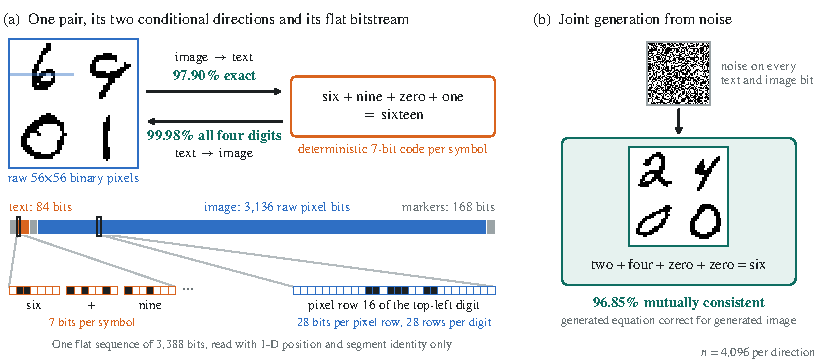
\includegraphics[width=\linewidth]{figures/mnist_sum/fig_mnist_sum_compact.pdf}
\caption{MNIST-Sum, an exactly auditable image--text control. (a) Four binarised MNIST digits and
their equation are written as one flat sequence of 3,388 bits: 3,136 raw pixel bits, 84 text
bits (twelve deterministic 7-bit symbol codes) and 168 marker bits, so neither side has a learned
tokenizer; the zoom-ins show actual bits of this pair. One 63.3M-parameter denoiser serves both conditional
directions by observing one half of the stream and denoising the other. Image$\rightarrow$text is
scored by exact string match; text$\rightarrow$image requires a fixed quadrant classifier to
recover all four requested digit identities. (b) With nothing observed, the same weights
co-generate an image and an equation from noise; a sample counts only if the generated equation
is correct for the generated image. Rates are over $n{=}4{,}096$ samples per direction; the
samples shown are fixed examples that illustrate, rather than estimate, these rates.}
\label{fig:mnist:sum}
\end{figure}

\textbf{One bitstream, no learned tokenizer.} Images enter as raw binary pixels and text as a
deterministic 40-symbol, 7-bit code; a pair becomes one flat sequence of 3,388 bits (3,136 pixel
bits, 84 text bits and 168 marker bits), which the denoiser reads in 28-bit positions. It receives
this flat sequence, its 1-D position and segment identity, but no pixel grid, 2-D attention structure, image encoder, text encoder or
modality-specific head. A single 63.3M-parameter model trained for 500K steps performs all three
directions; only the observed part of the stream changes.

\textbf{Result.} At $n{=}4{,}096$ per direction, image$\rightarrow$text is 97.90\% exact,
text$\rightarrow$image places all four requested digits correctly in 99.98\% of samples, and
joint co-generation from noise is 96.85\% mutually consistent (Figure~\ref{fig:mnist:sum}).
Held-out digit tuples reach 97.92\% image$\rightarrow$text, statistically indistinguishable from
seen tuples. The qualitative samples in the figure only illustrate these rates; the evidence is
the aggregate evaluation. Appendix~\ref{app:image:mnist} gives classifier calibration, confidence
intervals and the error decomposition. Having established the interface where it can be audited
exactly, the remaining experiments turn to the serious higher-scale settings: audio--text
(\S\ref{sec:exp:audio}) and protein sequence--structure (\S\ref{sec:exp:protein}).

\FloatBarrier

\else
\subsection{Image and text}
\label{sec:exp:imagetext}

Images and captions are where unified generative models are most often measured, and also where
the ingredients that usually carry them---a text-pretrained backbone, a frozen text encoder,
curated or re-captioned data---are hardest to separate from the modelling choice itself. We
therefore ask what the bitstream formulation transfers with none of them present. On an alt-text
corpus, though, every available metric is a proxy: FID and CMMD compare distributions, CLIP
compares embeddings, CIDEr compares $n$-grams, and none of them can say whether a co-generated
\emph{pair} actually agrees. We begin instead with a small corpus on which every direction has a
unique correct answer.

\begin{figure}[t]
\centering
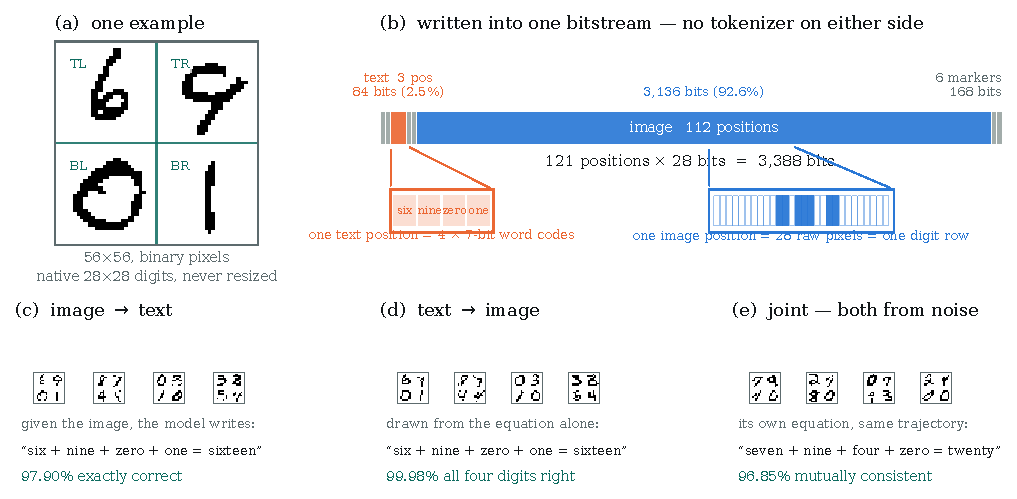
\includegraphics[width=\linewidth]{figures/mnist_sum/fig_mnist_sum_overview.pdf}
\caption{MNIST-Sum. (a) Four native $28{\times}28$ binarised digits on a $56{\times}56$ canvas,
never resized. (b) Image and text in a single 3{,}388-bit stream of 121 positions $\times$ 28
bits, with no tokenizer on either side---one text position holds four 7-bit word codes, one image
position holds 28 raw pixels, exactly one row of one digit. (c--e) The three directions, with
samples and their exact-match rates at $n{=}4{,}096$.}
\label{fig:mnist:sum}
\end{figure}

\textbf{MNIST-Sum: a ground truth for every direction, and no tokenizer on either side.} The corpus
pairs an image of four binarised MNIST digits \citep{image:mnist} in a $2{\times}2$ grid with the
raster-order equation and its sum, so each of image$\rightarrow$text, text$\rightarrow$image and
joint co-generation has a unique correct answer (Figure~\ref{fig:mnist:sum}). Neither modality is
tokenized: binary pixels ride as raw bits and the text uses a hand-specified 7-bit vocabulary, so
the framework is exercised with no modality-specific component at all. A 63.3M-parameter model
trained on the CC3M recipe unchanged writes the correct equation for a given image 97.90\% of the
time against a 6.52\% modal-sum baseline, and places all four digits correctly for a given
equation in 99.98\% of samples. The direction that matters is joint co-generation, where nothing
is given and both halves come from one trajectory: \textbf{96.85\%} of co-generated pairs carry an
equation exactly correct for the image produced beside it. Held-out digit tuples score
indistinguishably from training ones (Appendix~\ref{app:image:mnist}).

\textbf{Alt-text setup.} We train CoBit-CC3M (462M, $24\times1024$) on Conceptual Captions 3M
\citep{image:cc3m} ($\approx$2.9M pairs) and CoBit-CC12M (633M, $26\times1152$) on Conceptual 12M
\citep{image:cc12m} ($\approx$11.7M pairs, trained to 87\% of its planned step budget). Images are
tokenized by a
frozen Open-MAGVIT2 lookup-free quantiser \citep{image:magvit2,image:lfq} into 18-bit codes,
$16{\times}16$ ($f16$) for CC3M and $32{\times}32$ ($f8$) for CC12M; text uses \texttt{o200k}, and
a 19th namespace bit separates the two, so every position of either modality is one 19-bit token
(\S\ref{sec:method:multimodal}). Neither model sees MS-COCO \citep{image:mscoco}: every number
below is zero-shot under one fixed protocol (Appendix~\ref{app:image:protocol}). Text-only
pre-training, tokenizer surgery, auxiliary alignment losses and staged curricula are deliberately
absent; each is known to help, and we omit them so that the result measures what the unmodified
framework transfers.

\begin{table}[t]
\centering
\small
\setlength{\tabcolsep}{4.5pt}
\begin{tabular}{lrrrrrr}
\toprule
\textbf{Direction} & $n$ & Steps (NFE) & \textbf{FID}$\downarrow$ & \textbf{CMMD}$\downarrow$ & \textbf{CLIP}$\uparrow$ & \textbf{CIDEr}$\uparrow$ \\
\midrule
\multicolumn{7}{l}{\emph{CoBit-CC3M --- one set of weights (462M, $f16$, 256 image tokens)}}\\
text $\rightarrow$ image & 30{,}000 & 10 (20) & \textbf{18.48} & \textbf{18.41} & 27.73 & --- \\
image $\rightarrow$ text$^{\ast}$ & 5{,}000 & 256 (512) & --- & --- & 24.83 & \textbf{0.136} \\
joint, 10 / 256 steps & 30{,}000 & 10 / 256 & 50.19 / 61.95 & 41.53 / 46.80 & 23.10 / 25.67$^{\dagger}$ & --- \\
\midrule
\multicolumn{7}{l}{\emph{CoBit-CC12M --- one set of weights (633M, $f8$, 1{,}024 image tokens)}}\\
text $\rightarrow$ image & 30{,}000 & 16 (32) & \textbf{16.59} & \textbf{17.76} & 26.51 & --- \\
image $\rightarrow$ text$^{\ast}$ & 5{,}000 & 256 (512) & --- & --- & 22.98 & 0.057 \\
joint, 20 / 256 steps & 5{,}000 & 20 / 256 & 56.18 / 64.47 & 37.60 / 40.33 & 23.19 / 24.01$^{\dagger}$ & --- \\
\midrule
\emph{Floor of the FID column: two disjoint real draws} & 30{,}000 & & 2.35 & --- & --- & --- \\
\emph{\quad the same draw after the codec, $f16$ / $f8$} & 30{,}000 & & 2.94 / 2.55 & --- & --- & --- \\
\bottomrule
\end{tabular}
\caption{Zero-shot MS-COCO, all four generative directions from a single set of weights per model.
Each row is quoted at the step count best for that direction (\emph{Sampler} below); joint
generation has no single optimum, so both ends of its trade-off are shown. CLIP is ViT-B/32. The
last two rows are the floor of the FID column: a disjoint draw of real COCO images against the
same reference, and that draw after the tokenizer round-trip, so the codec's own share is 0.59 /
0.20 (Appendix~\ref{app:image:protocol}). $^{\ast}$CLIP and CIDEr come from separate runs at their
own guidance (3.0 / 2.0) against the COCO reference set and the Karpathy test split respectively.
$^{\dagger}$Pair coherence between the generated image and its caption, not comparable to the
conditional CLIP scores; FID of the joint rows is of the generated image half. FID is biased in
$n$ ($+5.3$ at $n{=}5{,}000$), so the CC12M joint rows are not FID-comparable to CC3M's.
Guidance, churn, ViT-L/14, SWD and precision/recall are in
Appendix~\ref{app:image:headline-full}.}
\label{tab:image:headline}
\end{table}

\begin{table}[t]
\centering
\small
\setlength{\tabcolsep}{4pt}
\begin{tabular}{lrrrr}
\toprule
\textbf{Model} & \textbf{Params} & \textbf{Pre-train pairs} & \textbf{FID-30K}$\downarrow$ & \textbf{GenEval}$\uparrow$ \\
\midrule
\multicolumn{5}{l}{\emph{CoBit (ours; from scratch, no pretrained components)}}\\
CoBit-CC3M & 462M & 2.9M & 18.48 & 0.249 \\
CoBit-CC12M & 633M & 11.7M & 16.59 & 0.222 \\
\midrule
\multicolumn{5}{l}{\emph{Same pre-training corpus (CC3M), zero-shot COCO}}\\
LAFITE \citep{image:lafite} & 75M ($+$CLIP) & 3.3M & 26.94 & --- \\
\midrule
\multicolumn{5}{l}{\emph{Unified image$+$text models}}\\
CoDI \citep{image:codi} & --- & 400M & 22.26 & 0.31 \\
SEED-X \citep{image:seedx} & 17B & --- & 14.99 & 0.49 \\
LWM \citep{image:lwm} & 7B & --- & 12.68 & 0.47 \\
UniDiffuser \citep{image:unidiffuser} & 952M & LAION-5B (subsets) & 9.71$^{\dagger}$ & --- \\
Show-o \citep{image:showo} & 1.3B & 35M & 9.24 & 0.68 \\
\midrule
\multicolumn{5}{l}{\emph{Text-to-image specialists}}\\
DALL$\cdot$E \citep{image:dalle} & 12B & 250M & 27.50 & --- \\
LDM \citep{image:ldm} & 1.4B & 400M & 12.63 & 0.37 \\
SD v1.5 \citep{image:ldm} & 0.9B & 2000M & 9.62 & 0.43 \\
PixArt-$\alpha$ \citep{image:pixart} & 0.6B & 25M & 7.32 & 0.48 \\
\bottomrule
\end{tabular}
\caption{Zero-shot MS-COCO FID-30K and GenEval against published systems, as printed in the cited
papers and the compilation tables of \citet{image:showo}, \citet{image:unidiffuser},
\citet{image:lafite} and \citet{image:geneval}. The rows are not strictly comparable and are not
meant to be ranked: parameter counts follow each source's own convention and exclude frozen
components inconsistently, the pair counts count different things, and the same nominal FID moves
by about a point between compilations. Appendix~\ref{app:image:repro} gives the per-row caveats
and the systems left out; Appendix~\ref{app:image:geneval} gives the GenEval breakdown and further
rows. $^{\dagger}$\citet{image:unidiffuser} draw 10K and 30K prompts for FID and CLIP score
without saying which is which.}
\label{tab:image:litcomparison}
\end{table}

\textbf{Results and placement.} Table~\ref{tab:image:headline} reports all four directions for
both models. Text$\rightarrow$image is the strongest, at zero-shot FID-30K \textbf{18.48} (NFE 20)
and \textbf{16.59}; neither is near the floor of that column, where two disjoint sets of real COCO
images already score 2.35 and the codec adds only 0.59 and 0.20, so the distance to larger systems
lies in the model and not in the token space---Figure~\ref{fig:image:gap} shows the same thing by
eye. The text-emitting directions are weaker, at CIDEr 0.136 and image$\rightarrow$text CLIP
24.83. Joint co-generation is harder again (FID 50.19): with no prompt the model samples its own
CC3M-like distribution rather than COCO's, and the distributional metrics charge it for the
difference---but pair coherence 25.67 is about as high as a conditional caption's agreement with
its own image (24.83), so the shortfall is in matching the evaluation corpus, not in keeping the
modalities together. Table~\ref{tab:image:litcomparison} places this among published zero-shot
MS-COCO numbers. Against LAFITE, the one system trained on the same corpus under the same
protocol, FID improves by 8.46 without its frozen CLIP encoder; among unified image$+$text models
we sit between CoDI and SEED-X, and ahead of the 12B-parameter DALL$\cdot$E specialist. Every
system with a lower FID uses pretrained language or vision components and most train on far more
paired data. Compositional prompt following is where the gap is widest (GenEval 0.249 and 0.222, either side of
minDALL$\cdot$E's 0.23 and far below the LLM-backed unified models;
Appendix~\ref{app:image:geneval}), and for captioning there is no
published zero-shot COCO baseline at all: COCO-trained specialists reach CIDEr 1.02--1.40 against
our 0.136. The claim is capable transfer, not a leaderboard entry.

\textbf{Sampler: the two modalities want step counts $\mathbf{25\times}$ apart.} Sweeping the step
count from 4 to 512 on the same weights, text$\rightarrow$image FID and CMMD minimise at 10 steps
for CC3M and 16--20 for CC12M and degrade monotonically beyond---the conventional 256 steps costs
4.06 FID for $25.6\times$ the compute---while captioning rises from CIDEr 0.013 at 10 steps to
0.136 at 256; the joint direction shows both effects inside single samples, which is why
Table~\ref{tab:image:headline} quotes it at both ends. The image-side optimum is driven by the
distributional metrics specifically: CLIP moves by under 0.1 between 8 and 256 steps and GenEval
by under 0.01 across the same $25\times$ range, so the semantic metrics neither corroborate it nor
contradict it. None of this modifies the framework: the step count, like churn and guidance, is an
inference-time hyperparameter set per direction on the same weights, and such sampler settings are
the only thing that had to be adapted per modality (Appendix~\ref{app:image:sampler}).

\textbf{Scaling, and limitations.} Moving to CC12M---$4\times$ the pairs, $\approx8.7\times$ the
compute and a better codec---improves images and degrades text: FID falls
$18.48\rightarrow16.59$, a margin that survives subtracting each codec's own contribution
($17.90$ versus $16.39$), while captioning CIDEr falls $0.136\rightarrow0.057$ at matched
settings. That split is what noisier CC12M alt-text predicts and what uniform undertraining does
not, though it remains an inference across metrics rather than a measurement of caption quality
(Appendix~\ref{app:image:scaling}). The two weaknesses have the same shape. On GenEval, single
objects render 80\% of the time and colours 46\% while position and attribute binding sit near
zero, and the score is flat between each model's image optimum and 256 steps, so it is the
model's ceiling rather than a sampler artefact. Captioning is weak in absolute terms, and the outputs are fluent
CC3M-style alt-text scored against COCO's terse references, which the $n$-gram metrics penalise
almost regardless of content (RefCLIPScore \citep{image:clipscore} 0.661;
Appendix~\ref{app:image:captioning}). Both are consistent with CC3M alt-text rarely specifying
relations or attribute bindings, and both are exactly what the omitted ingredients are expected to
buy. That is the point of the experiment: it shows what unmodified transfer does and does not
provide.

\fi
\subsection{Audio and text}
\label{sec:exp:audio}

\textbf{Overview.} Joint text-audio modeling precisely fits the discrete-continuous combination bitstream diffusion is well-suited for: text represents a utterance as a discrete sequence and speech as a continuous signal with richer information, including speaker identity, emotion and background noise. The relationship between the two modalities can be easily measured through the alignment of their content. We follow the speech language modeling paradigm \citep{audio:twist, audio:spirit-lm}, where speech is tokenized into discrete units and generation occurs in terms of text and speech tokens, introducing the first non-autoregressive speech language model (SLM) in the process.

\textbf{Setup.} We train two models: CoBit-LibriTTS (134M, $12\times768$) on LibriTTS \citep{audio:libritts} (354K pairs, 140K steps) and CoBit-MLS (633M, $26\times1152$) on both LibriTTS and MLS-English \citep{audio:mls} (11.2M pairs, $1.2\times10^6$ steps). We quantize audio with the FSQ-based StableCodec \texttt{1x46656} that produces 25 tokens per second (budget of 800 and 500 tokens, respectively), combined with a fixed-length (32) global speaker representation from BiCodec-global \citep{audio:spark-tts}. Speaker tokens are included as a conditioning signal for generation and are omitted during audio decoding. Using \texttt{o200k} for text (budget of 168 and 100 tokens, respectively), the full vocabulary fits into 18 bits. Training additionally includes a prompt-conditional regime, with equal effort (0.25) allocated to each setting. Evaluation is conducted on LibriSpeech-PC \citep{audio:librispeech-pc} and the SALMON benchmark. Text pre-training and speaker conditioning on the decoder are omitted. Warm-initializing CoBit from a pre-trained text checkpoint is straightforward in principle: it mainly required adapting the components that are tied to the sequence length and the vocabulary bit-width. We expect both changes to close the remaining performance gap and leave their implementation to a dedicated line of work on text-audio CoBit.

\begin{figure}[ht]
    \centering
    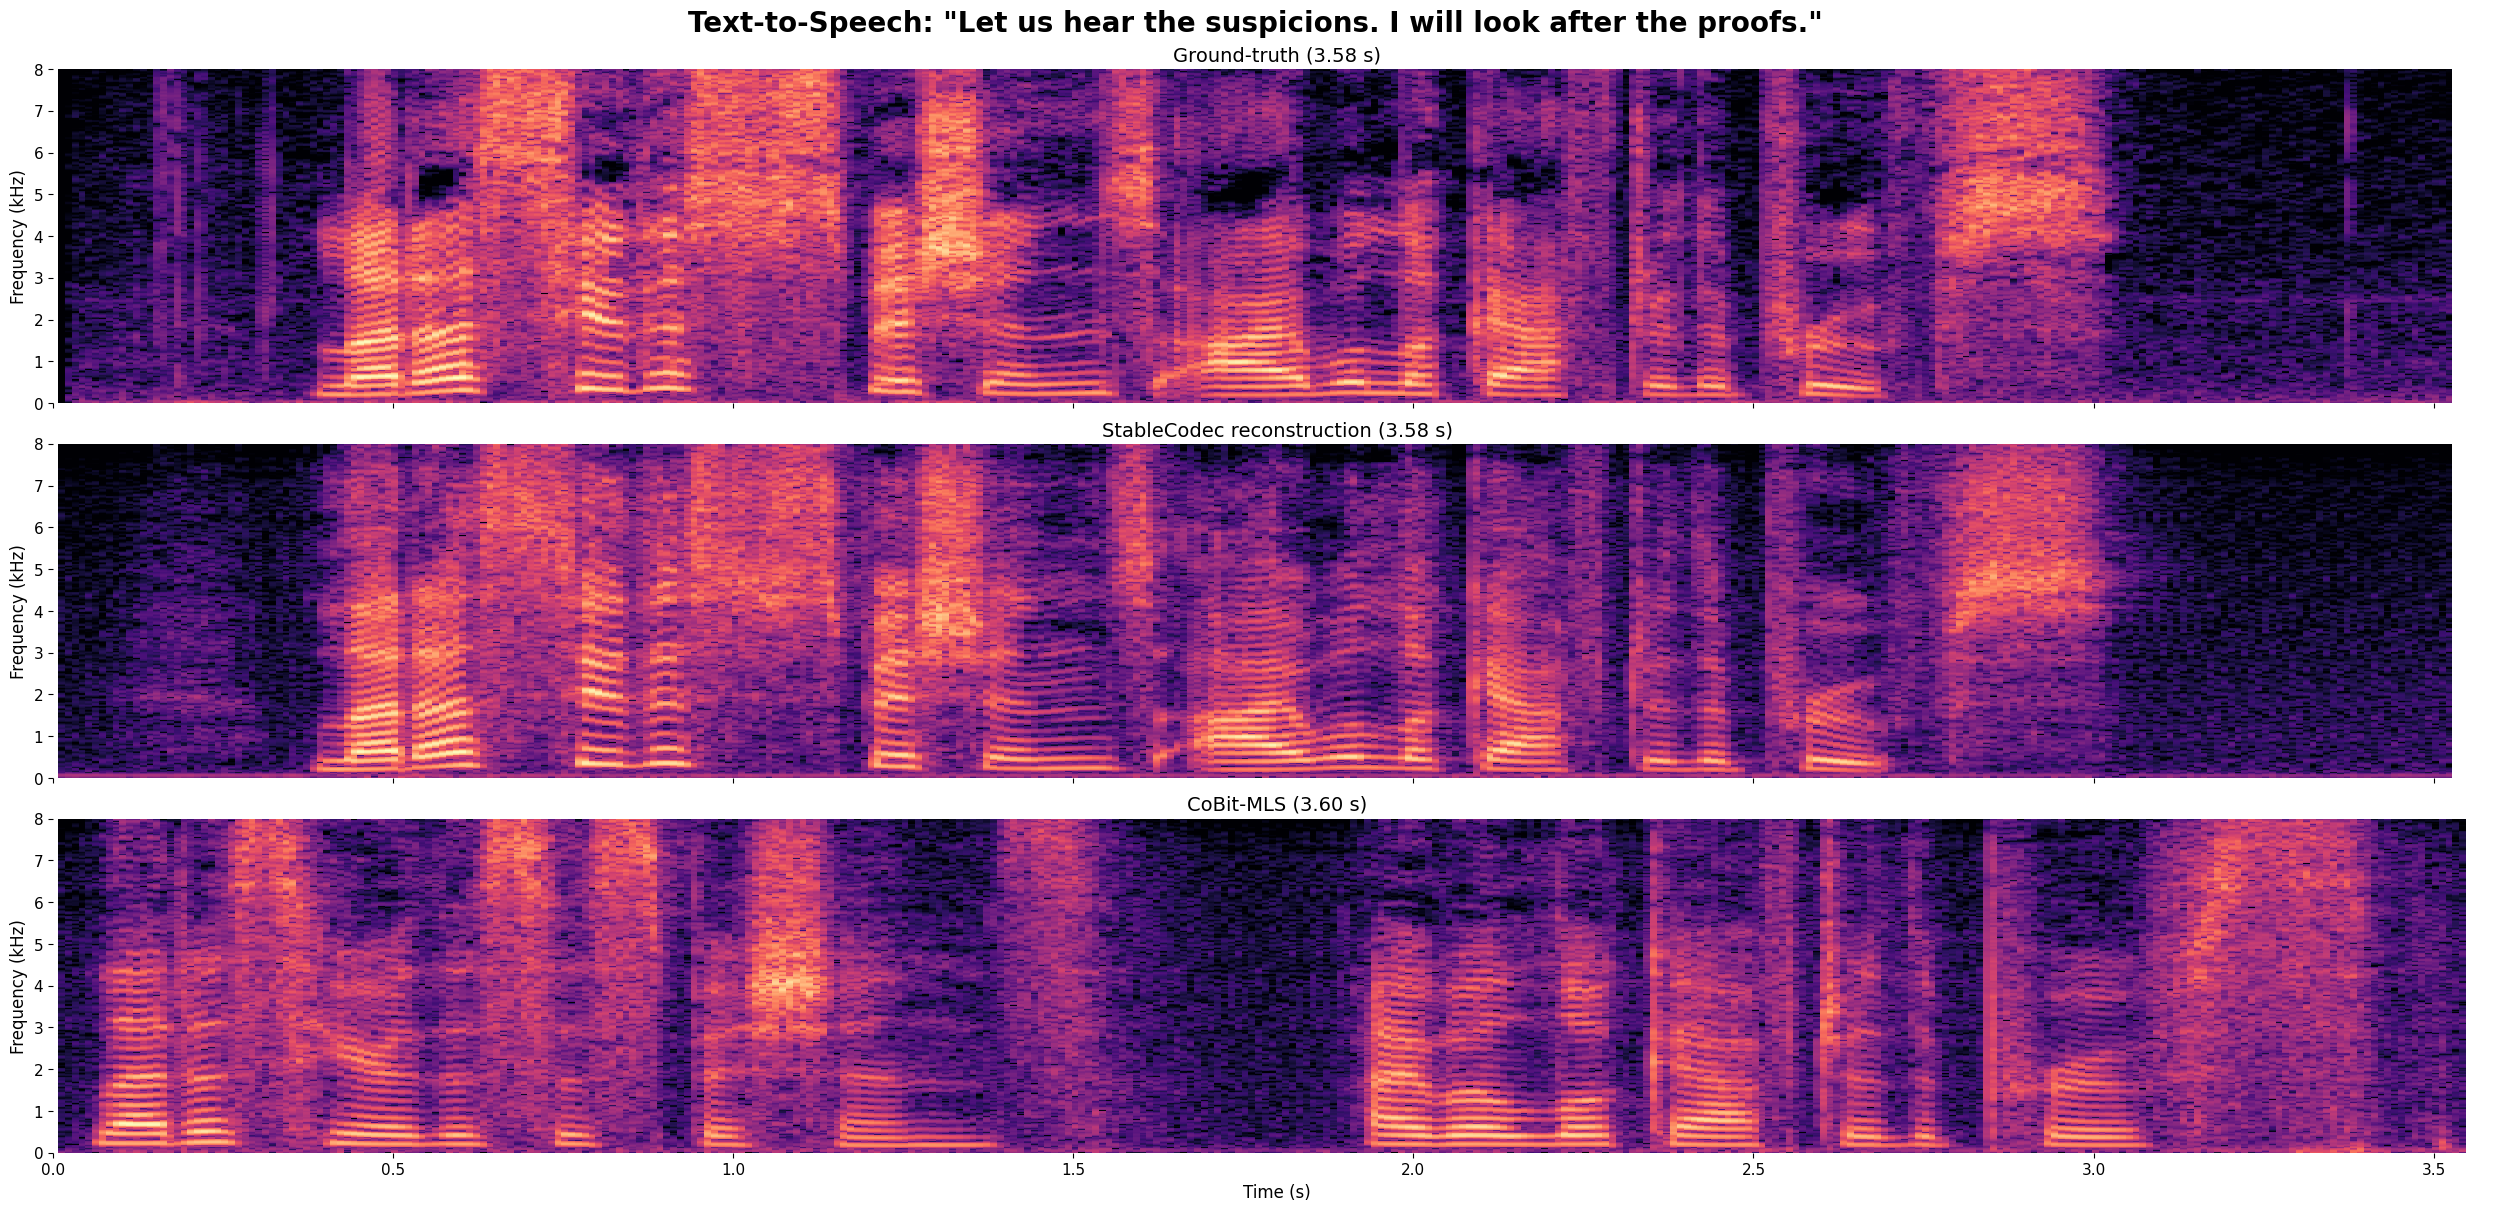
\includegraphics[width=\linewidth]{figures/audio/tts.png}
    \caption{Text-to-speech generation with CoBit-MLS. Given text and speaker tokens (extracted from a held-out example), the model is tasked with generating the speech part of the sequence. The top mel-spectrogram corresponds to the ground truth waveform, the middle one to the StableCodec reconstruction , and the bottom mel-spectrogram to the generated audio by the 633M parameter bitstream diffusion model. The tokenizer introduces visible artifacts, especially for high frequency. CoBit generation spreads the utterance across a longer time-frame, without leading and trailing silence, replicating similar frequency patterns. The only exception is the gap between 1.7 and 1.9 seconds, which corresponds to the change of sentences.}
    \label{fig:audio:tts-spectrogram}
\end{figure}

\textbf{Results.} Co-generation and conditional directions are reported in Table \ref{tab:audio:headline}, using the same weights for all tasks. CoBit-MLS can co-generate text and audio consistently, achieving a cross-modal WER of 3.5. An UTMOS score of 3.77 suggests natural-sounding audio, despite sampling the speaker identity from scratch. The content also remains highly plausible and syntactically solid in terms of perplexity under an external LM. Both models are considerably stronger in speech-emitting than text-emitting generation. Mel-spectrograms for a text-to-speech example are visualized in Figure \ref{fig:audio:tts-spectrogram}. In speech continuation, CoBit samples acoustically and linguistically grounded audio, yet the struggle to preserve thematic content. StableCodec sets an upper bound for audio performance, with CoBit-MLS recovering almost reconstruction-level SpkSim for speech continuation.\footnote{Inspect text-audio-examples online: \url{https://demo-2546.github.io/cobit-text-audio-samples/}.}

% \begin{table}[t]
% \centering
% \small
% \setlength{\tabcolsep}{4.5pt}
% \begin{tabular}{lrrrrrr}
% \toprule
% \textbf{Direction} & $n$ & Steps (NFE) & \textbf{WER}$\downarrow$ & \textbf{CER}$\downarrow$ & \textbf{UTMOS}$\uparrow$ & \textbf{GenPPL-Speech}$\downarrow$ \\
% \midrule
% \multicolumn{7}{l}{\emph{CoBit-LibriTTS --- one set of weights (134M, 800 speech tokens)}}\\
% text $\rightarrow$ speech & 2{,}294 & 512 (1024) & 11.7 & 8.1 & 3.31 & ---- \\
% speech $\rightarrow$ text & 2{,}294 & 512 (1024) & 23.3 / 38 & 15.3 / 24.1 & --- & --- \\
% joint & 1{,}024 & 256 (256) & 19.9 & 13.3 & 3.02 & 377.2 \\
% \midrule
% \multicolumn{7}{l}{\emph{CoBit-MLS --- one set of weights (633M, 500 speech tokens)}}\\
% text $\rightarrow$ speech & 2{,}294 & 512 (1024) & 5.3 & 4.1 & 4 & --- \\
% speech $\rightarrow$ text & 2{,}294 & 512 (1024) & 8.2 / 22 & 4.3 / 13.1 & --- & --- \\
% joint & 1{,}024 & 512 (512) & 3.5 & 1.8 & 3.77 & 133.3 \\
% \bottomrule
% \end{tabular}
% \caption{Joint and cross-conditional generative directions from a single set of weights per model for text-audio experiments. Each conditional row is quoted at the best step count for that direction, evaluated on LibriSpeech-PC. Generated audio is transcribed with Whisper-large. Per-direction guidance and churn are listed in Appendix \ref{app:audio:protocol}; co-generation uses $\gamma=0.175$. Text-to-speech evaluation is on test-clean; the two scores for speech-to-text refer to test-clean and test-other, respectively.}
% \label{tab:audio:headline}
% \end{table}

\begin{table}[t]
\centering
\footnotesize
\setlength{\tabcolsep}{4pt}
\resizebox{\linewidth}{!}{%
\begin{tabular}{lrrrrrrrr}
\toprule
\textbf{Direction} & $n$ & Steps (NFE) & \textbf{WER}$\downarrow$ & \textbf{CER}$\downarrow$ & \textbf{UTMOS}$\uparrow$ & \textbf{SpkSim}$\uparrow$ & \textbf{FSD}$\downarrow$ &\textbf{GenPPL}$\downarrow$ \\
\midrule
\multicolumn{7}{l}{\emph{CoBit-LibriTTS --- one set of weights (134M, 800 speech tokens)}}\\
text $\rightarrow$ speech & 2{,}294 & 512 (1024) & 11.7 & 8.1 & 3.31 & 0.19 & --- & --- \\
speech $\rightarrow$ text & 2{,}294 / 2{,}813 & 512 (1024) & 23.3 / 38 & 15.3 / 24.1 & --- & --- & --- & --- \\
speech continuation & 1{,}936 & 512 (1024) & --- & --- & 2.82 & 0.21 & 2,373 / 40.5 & 152.1 \\
joint & 1{,}024 & 256 (256) & 19.9 & 13.3 & 3.02 & --- & --- & 509.6 / 377.2 \\
\midrule
\multicolumn{7}{l}{\emph{CoBit-MLS --- one set of weights (633M, 500 speech tokens)}}\\
text $\rightarrow$ speech & 2{,}294 & 512 (1024) & 5.3 & 4.1 & 4 & 0.27 & --- & --- \\
speech $\rightarrow$ text & 2{,}294 / 2{,}813 & 512 (1024) & 8.2 / 22 & 4.3 / 13.1 & --- & --- & --- & --- \\
speech continuation & 1{,}036 & 512 (1024) & --- & --- & 3.89 & 0.34 & 2,386 / 13 & 83.6 \\
joint & 1{,}024 & 512 (512) & 3.5 & 1.8 & 3.77 & --- & --- & 252.4 / 133.3 \\
\bottomrule
\end{tabular}%
}
\caption{All text-audio generative directions from a single set of weights per model. Each conditional row is quoted at the best step count for that direction, evaluated on LibriSpeech-PC. Generated audio is transcribed with Whisper-large. Per-direction guidance and churn are listed in Appendix \ref{app:audio:protocol}; co-generation uses $\gamma=0.175$. Text-to-speech and speech continuation evaluation is on test-clean; the two scores for speech-to-text refer to test-clean and test-other, respectively. For FSD, the two separate metrics refer to FSD-wlm and FSD-e2v, respectively. For co-generation, generative perplexity is reported for both the text (left) and the audio (right) streams.}
\label{tab:audio:headline}
\end{table}

\textbf{Comparison to prior work.} Appendix \ref{app:audio:results} places CoBit among autoregressive SLMs and other baselines for all tasks. The capabilities of bitstream diffusion are best demonstrated in speech continuation, where CoBit-MLS outperforms all baselines except TASLM-Embed across audio-based metrics and generative perplexity. Modifying the sampler settings, CoBit-MLS can surpass even TASLM-Embed in terms of expressiveness (Appendix \ref{app:audio:sampler}.  LLM-as-a-Judge is CoBit's weakest overall evaluation (see Appendix \ref{app:audio:llm} for further discussion). In SALMON-based evaluation, CoBit-MLS scores better on average than all other text-speech SLMs, but cannot match speech-only models. While it remains competitive on the voice-related tasks, it is worse than Mimi-based models, like Flow-SLM and Llama-Mimi on noise-related ones. In text-to-speech, CoBit-MLS surpasses SpiritLM on CER (4.1 to 6.7) and approaches Moshi on WER (5.3 to 4.7), despite being 10 times smaller. However, despite the consistency and naturalness of generated audio, speaker characteristics are not reproduced to the same level as by the ASR-TTS hybrid GPA-v1.5 \citep{audio:gpa} where the decoder is not conditioned on the speaker. Speech recognition is the task where the absence of text-only training matters the most, with CoBit having the worst performance relative to baselines.

\textbf{Sampler: integration steps and guidance aid semantics.} Higher NFE are most critical when the model is tasked with producing novel semantics (joint generation and speech continuation): generative perplexity decreases near-monotonically as the step count increases. For cross-modal tasks on the other hand, performance plateaus at 32 integration steps, with higher counts offering mild improvements. The same perplexity pattern for speech continuation is observed when increasing the guidance scale as well. Guidance also plays a crucial role for alignment in cross-modal directions, especially text-to-speech. However, increasing the guidance scale has a negative effect on frame-level fidelity and expressiveness: minimal and no guidance settings score the lowest reported FSD-e2v figure surpassing all baselines, along with improved FSD-wlm scores (Appendix \ref{app:audio:sampler}).

\textbf{Limitations.} Thematic extrapolation is the model's worst aspect, with CoBit continuations often receiving the lowest possible score. Speech recognition is the overall weakest task, with a large portion of the errors occurring at word-level (CoBit-MLS: WER $\simeq2\times$ CER on test-clean). These limitations are strongly tied to the lack of text pre-training. Imprecise speaker replication is directly associated with the low SpkSim ceiling of StableCodec reconstructions and, for text-to-speech in particular, the lack of speaker conditioning on the audio decoder. While such design choices are well-established in SLM literature, they are not included in this work to demonstrate what the generalized bitstream diffusion framework can achieve off-the-shelf.

\begingroup
\raggedbottom

\subsection{Protein sequence and structure}
\label{sec:exp:protein}

% We trained a 393M parameter model from scratch on PDB/AFDB--swissProt pairs with sequence replay. Each residue is formed by an aligned 18-bit patch: five amino-acid bits and thirteen sign bits from the fozen DPLM-2 lookup-free quantiser \citep{protein:dplm2}.  The 5-bit sequence channel has capacity for 32 symbols, but the deconding is contrained to the 20 canonical amino acids. This compact representation retains the full vocabulary of $(2^{13}=8192)$ structrual codes. Thus, the model preserves structure expressivity of DPLM-2 whiile supporting residue-aligned joint sequence-structure generation. \bruno{Details about dataset splits etc to be in the appendix}

Unlike text, image, and audio multi-modality, whose correspondence is primarily semantic, a protein sequence and its three-dimensional structure are physically coupled descriptions. We ask whether the bitstream formulation can learn the coupled modalities of protein sequence and structure by training CoBit from scratch on 216,237 PDB/AFDB-SwissProt \citep{protein:pdb, protein:afdb} pairs with 20\% sequence replay. Each residue aligns five amino-acid bits with thirteen signs from the frozen DPLM-2 lookup-free quantiser (LFQ) \citep{protein:dplm2}. Decoding retains the 20 canonical amino acids and all $2^{13}$ structural codes. The common binary interface lets one denoiser learn sequence--structure dependencies while the frozen codec recovers backbone coordinates. Data, splits, and tokenisation are detailed in Appendices~\ref{app:protein:protocol} and~\ref{app:protein:training}.

% \par\addvspace{6pt}\noindent
%     \begin{minipage}{\linewidth}
%     \makeatletter\def\@captype{figure}\makeatother
%     \centering
%     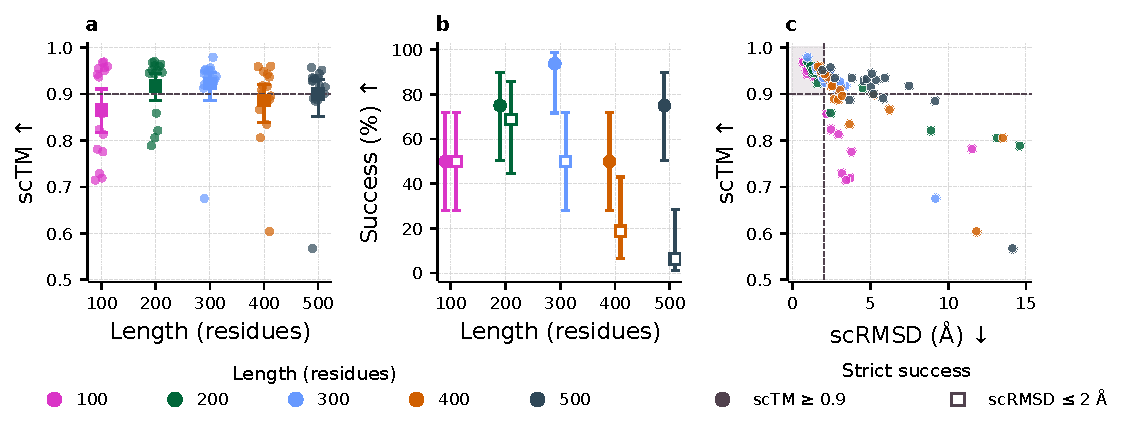
\includegraphics[width=\linewidth]{figures/protein/protein_multimodal_evidence.pdf}
%     \caption{Backbone quality from denoised bits: (a) scTM by length, (b) strict success
%     by length, and (c) fold similarity versus coordinate error. Colours denote length. 80 backbones each receive one ProteinMPNN redesign and ESMFold refold. Intervals are 95\%. Shading marks both strict criteria.}
%     \label{fig:protein:multimodal}
%     \label{fig:protein:strict}
% \end{minipage}\par\addvspace{6pt} 

\begin{figure}[!t]
    \centering
    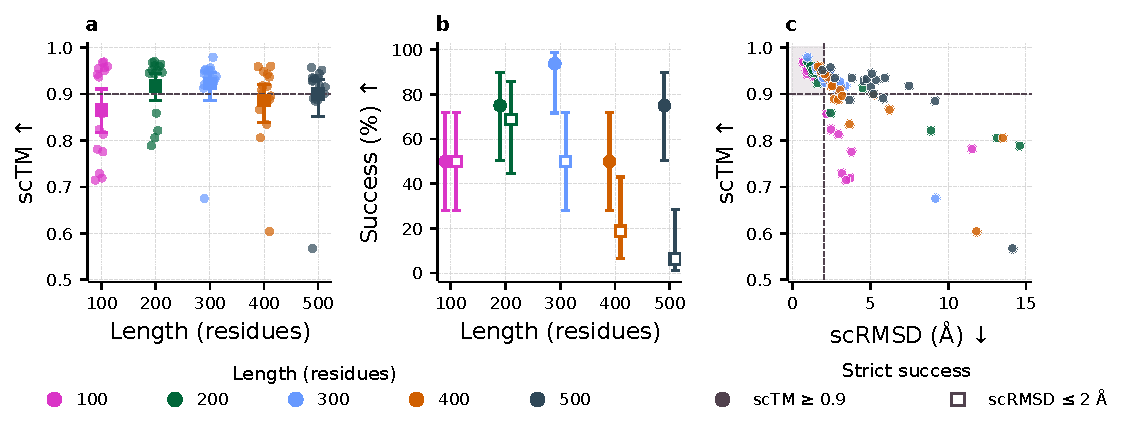
\includegraphics[width=.8\linewidth]{figures/protein/protein_multimodal_evidence.pdf}
    \caption{Backbone quality from denoised bits: (a) scTM by length, (b) strict success
    by length, and (c) fold similarity versus coordinate error. Colours denote length. 100 backbones (20 per length) each receive one ProteinMPNN redesign and ESMFold refold. Intervals are 95\%. Shading marks both strict criteria.}
    \label{fig:protein:multimodal}
    \label{fig:protein:strict}
\end{figure}

% We ask whether one shared bitstream formulation can learn representations of protein sequences and structures. Unlike text, image, and audio multimodality, whose correspondence is primarily semantic, a protein sequence and it's three-dimensional structure are physically coupled descriptions of the same molecualr system. 

% In a given environment,. the amino-acid sequences shapes the protein's free energy landscape and accesible conformation ensemble \cite{protein:anfinsen} while a target backbone restricts the sequences likely to adopt that fold \citep{protein:proteinMPNN}. 

\textbf{Setup.} Clamping either channel gives inverse or forward folding while leaving both free enables joint generation, without task-specific fine-tuning or multiple sequence alignments as input (Appendix~\ref{app:protein:metrics}). Our evaluations were based on entropic DDIM with $50$ grid points, conditional CFG $5$ and no unconditional guidance. Under these settings, mean recovery is $44.10\%$ on 128 CATH 4.3 validation targets and forward TM is $.554$ on $183$ CAMEO targets \citep{protein:cath,protein:cameo,protein:tmscore}. These results test bidirectional learning through one shared bitstream objective. For $100$ generated backbones ($20$ per length, 100--500), one ProteinMPNN redesign and ESMFold refold give mean scTM $.899$ \citep{protein:proteinmpnn,protein:esmfold}. Figure~\ref{fig:protein:multimodal} shows fold similarity across lengths while Figure~\ref{fig:protein:bestgallery} shows the best backbones per length-bucket. We assess backbone recovery after redesign and refolding using scTM  $\geq.9$ ($D_{\mathrm{TM}}$) for overall fold agreement and scRMSD $\leq2$\,\AA{} ($D_{\mathrm{RMSD}}$) for close coordinate agreement. Full metrics and sampling analysis are in Appendices~\ref{app:protein:metrics} and~\ref{app:protein:pareto}. 

Directly refolding CoBit's own sequences for the same 80 pairs gives mean scTM $.911$, with $D_{\rm TM}=69\%$ and $D_{\rm RMSD}=41\%$ (Table~\ref{tab:protein:direct}; Appendix~\ref{app:protein:direct}). This supports sequence--structure consistency at the fold level, despite lower coordinate-level success.


% \textbf{Learning the joint representation.} Clamping one modality gives forward or inverse folding. Leaving both free gives joint generation. \bruno{add the figure for the overview} show the two conditional directions and the generated-backbone evaluation. Information aboout training, evaluation, and the tokenizer can be found in Appendix~\ref{app:protein:protocol}. 

% \par\addvspace{6pt}\noindent
%     \begin{minipage}{\linewidth}
%     \makeatletter\def\@captype{figure}\makeatother
%     \centering
%     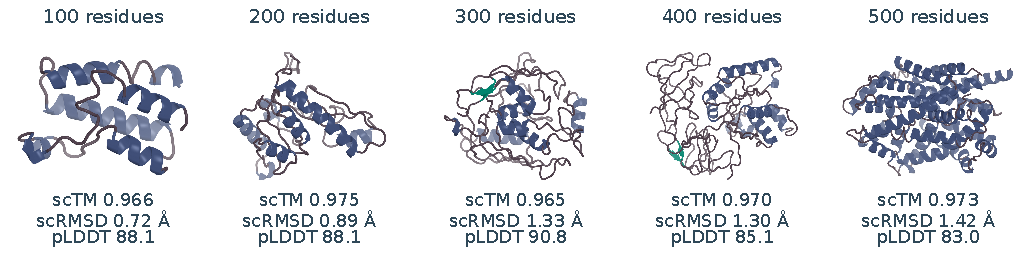
\includegraphics[width=.99\linewidth]{figures/protein/protein_pymol_best_grid.pdf}
%     \caption{Selected CoBit backbones, rendered with PyMOL \citep{protein:pymol}.
%     Highest scTM at each displayed length among samples with scRMSD $\leq2$\,\AA{};
%     scores use ProteinMPNN/ESMFold. pLDDT is predicted confidence.}
%     \label{fig:protein:bestgallery}
% \end{minipage}\par\addvspace{6pt}
\par\addvspace{6pt}\noindent
    \begin{minipage}{\linewidth}
    \makeatletter\def\@captype{figure}\makeatother
    \centering
    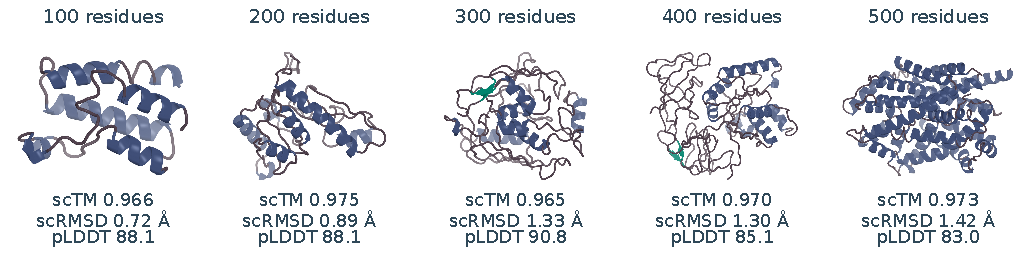
\includegraphics[width=.99\linewidth]{figures/protein/protein_pymol_best_grid.pdf}
    \caption{Selected CoBit backbones, rendered with PyMOL \citep{protein:pymol}.
%     Highest scTM at each displayed length among samples with scRMSD $\leq2$\,\AA{};
    Highest scTM among 20 samples at each displayed length with scRMSD $\leq2$\,\AA{};
    % scores use ProteinMPNN/ESMFold. pLDDT is predicted confidence.
    scores use ProteinMPNN/ESMFold. pLDDT is refold confidence.}
    \label{fig:protein:bestgallery}
\end{minipage}\par\addvspace{6pt}



% Sequence constrains the energy landscape and conformational ensemble \bruno{ cite affinsen....}, while structure constrains funcional vability. Hence, protein co-design goes byeyond cross-modal aligment, but joint generation over discrete sequence and continuous 3D geometry can be achieved with respect to geometric, chemical, thermodynamic and functional constraints intrinsic to these modalities \bruno{Cite Jumper et al.  }. 

% Figures~\ref{fig:protein:strict} and~\ref{fig:protein:lengthdist} show length-dependent quality: high fold similarity does not always imply low coordinate error. Figure~\ref{fig:protein:secondary} shows coarse secondary-structure proportions close

% Protein co-design there requires more than cross-modal semantic alignment because the structure and sequence must be mutually compatible. Cobit addesses this problem by jointly denoising discrete amino0acid and structural codes, with the structural codes being subsequently decoded into continuous backbone coordinates. Structural comparability can be assessed computionally through sequence refolding \citep{protein:jumper, protein:esmfold} whereas thermodynamic stability and biological function require additional computational or even experimental validation \cite{protein:rfdiffusion}, which is beyond the scope of this work. 

\textbf{Bitstream capability versus protein optimisation.} We compare CoBit's bitstream formulation against protein-specific models. Table~\ref{tab:protein:baselines} places CoBit alongside the models evaluated by \citet{protein:simpledesign}, following their published one-redesign procedure with 100 samples. MultiFlow \citep{campbell2024multiflow} leads on the strict criteria with a 21.8M-parameter model that uses explicit geometric learning and designability distillation. On the other hand, CoBit tests the common bit objective with an existing codec and paired-data recipe. Its sequence replay supplies unpaired examples unlike MultiFlow's designability distillation and without direct geometric supervision. Appendix~\ref{app:protein:comparison} explains the training differences and MultiFlow's distillation ablation in detail.


\par\addvspace{6pt}\noindent
\begin{minipage}{\linewidth}
\makeatletter\def\@captype{table}\makeatother
\centering
\begin{minipage}[t]{.55\linewidth}
\vspace{0pt}
\caption{Backbone designability (\%) with one ProteinMPNN redesign and ESMFold.
% Training data and evaluation settings differ across studies. Published baselines: \citet{protein:simpledesign}; G: general bitstream framework; P: protein-specific generator.}
Training data and evaluation settings differ across studies. Published PMPNN1 baselines: \citet{protein:simpledesign}; G: general bitstream framework; P: protein-specific generator.}
\label{tab:protein:baselines}
\label{tab:protein:literaturemain}
\centering
\fontsize{8}{9.5}\selectfont
\setlength{\tabcolsep}{2pt}
\begin{tabular}{@{}rlcrrr@{}}
\toprule
ID & Model & Scope & $n$ & $D_{\rm RMSD}$ & $D_{\rm TM}$ \\
\midrule
\multicolumn{6}{@{}l}{\emph{Our evaluation: joint bitstream generator}} \\
% 1 & CoBit & G & 80 & 38.8 & 68.8 \\
1 & CoBit & G & 100 & 36.0 & 75.0 \\
\midrule
\multicolumn{6}{@{}l}{\emph{Published evaluation: Lu et al. (2026)}} \\
\addlinespace
\multicolumn{6}{@{}l}{Joint generators: discrete structural codes} \\
2 & DPLM-2 (650M) & P & 100 & 31.0 & 48.0 \\
3 & ESM3 Open (sequence first) & P & 100 & 17.0 & 19.0 \\
4 & ESM3 Open (structure first) & P & 100 & 3.0 & 4.0 \\
\addlinespace
\multicolumn{6}{@{}l}{Joint generators: explicit / partially latent geometry} \\
5 & MultiFlow & P & 100 & 86.0 & 90.0 \\
6 & La-Proteina (no-triangle) & P & 100 & 84.0 & 86.0 \\
7 & La-Proteina (triangle) & P & 100 & 84.0 & 88.0 \\
8 & SimpleDesign & P & 100 & 44.0 & 63.0 \\
9 & ProtPardelle & P & 100 & 42.0 & 41.0 \\
10 & ProtPardelle-1c & P & 100 & 52.0 & 53.0 \\
11 & ProteinGenerator & P & 100 & 42.0 & 46.0 \\
\addlinespace
\multicolumn{6}{@{}l}{Structure generators} \\
12 & Proteina & P & 100 & 46.0 & 50.0 \\
13 & RFdiffusion & P & 100 & 49.0 & 54.0 \\
14 & FrameFlow & P & 100 & 46.0 & 49.0 \\
\bottomrule
\end{tabular}
\end{minipage}\hfill
\begin{minipage}[t]{.43\linewidth}
\vspace{0pt}
\makeatletter\def\@captype{figure}\makeatother
\caption{Visual representation of the rates from Table~\ref{tab:protein:baselines}. CoBit captures how proteins fold overall, but is less accurate on fine structural detail.}
\label{fig:protein:modelmap}
\centering
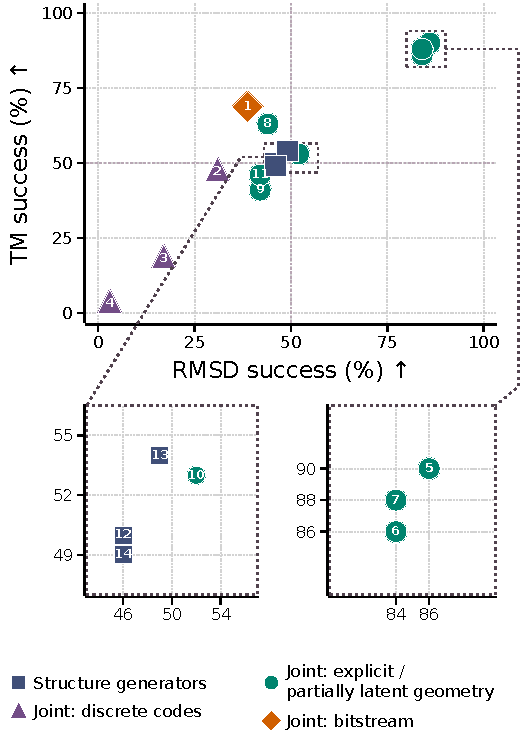
\includegraphics[width=\linewidth]{figures/protein/protein_model_designability_map.pdf}
\end{minipage}
\par\smallskip
\end{minipage}\par\addvspace{6pt}

A dedicated protein study can test that coupling and stronger supervision while testing scalability for biological tasks such as binder--linker design with laboratory (wet lab) validation. CoBit's stronger fold-level ($D_{\mathrm{TM}}$) than coordinate-level ($D_{\mathrm{RMSD}}$) success indicates that denoising structural bits captures useful protein organization information and that geometric precision can be further improved in a dedicated protein-training work, but this is highly dependent, in our case, to protein length and training set availability as shown in Figure~\ref{fig:protein:strict}. The present metrics indicate modeling quality, but establishing biological function requires additional setups and experiments. 

% Under the same training regime, we reach 44.10\% mean amino-avid recovery on CATH 4.3 validation and $.554$ mean forward TM-score \bruno{cite tm-score} on CAMEO 2022 \bruno{cite}, and $0.899$ mean backbone scTM (Table~\ref{tab:protein:headline}). 

% \bruno{Simplify image / reduce space}
% \begin{figure}[t]
%     \centering
%     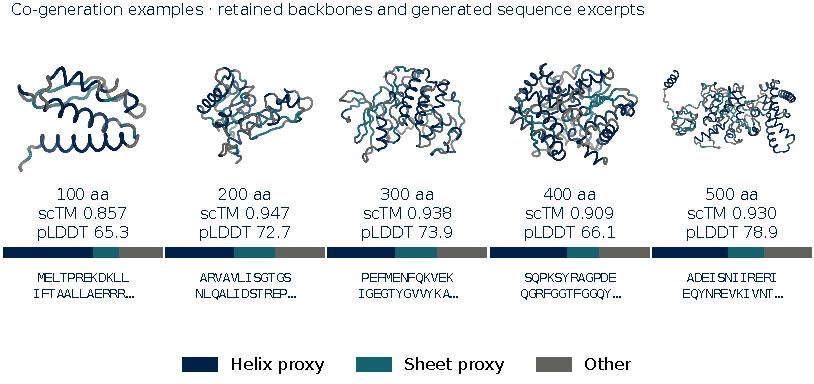
\includegraphics[width=\linewidth]{figures/protein/protein_pymol_gallery.pdf}
%     \caption{Placeholder}
%     \label{fig:protein-pymol-gallery}
% \end{figure}

% % \begin{table}[h!]
% % \centering
% %     \caption{}
% % \label{tab:protein:headline}
% % \small
% % \setlength{\tabcolsep}{4pt}
% % \begin{tabular}{llrl}
% % \toprule
% % Task & Evaluation & $n$ & Results $\uparrow$ \\
% % \midrule
% %     Inverse folding & CATH validation & 128 & AAR 44.10\%; scTM .739 \\
% %     Forward folding & CAMEO 2022 & 183 & TM .554; lDDT .541 \\
% %     Generated backbones & Lengths 100--500 & 80 & scTM .899; $D_{\rm TM}$ 68.75\% \\
% % \bottomrule
% % \end{tabular}
% % \end{table}

% % \begin{table}[h!]
% % \centering
% % \caption{One CoBit model for protein sequence and structure generation.
% % All-candidate means describe typical quality; best-of-four scores describe
% % selection with the native reference.}
% % \label{tab:protein:headline}
% % \small
% % \setlength{\tabcolsep}{3pt}
% % \begin{tabular*}{\linewidth}{@{\extracolsep{\fill}}lrrrrrr@{}}
% % \toprule
% % \multicolumn{7}{@{}l}{\textbf{Inverse folding} --- CATH validation: 128 targets, 512 sequences} \\
% % & & \multicolumn{2}{c}{AAR (\%) $\uparrow$} & \multicolumn{3}{c}{First sequence only: 128 refolds} \\
% % \cmidrule(lr){3-4}\cmidrule(l){5-7}
% % Model & Params (M) & Mean (all) & Best of 4 & scTM $\uparrow$ & scRMSD (\AA) $\downarrow$ & pLDDT $\uparrow$ \\
% % \midrule
% % CoBit & 396.23 & 44.10 & 45.20 & .739 & 6.104 & 61.80 \\
% % \bottomrule
% % \end{tabular*}
% % \end{table}

% \begin{table}[h!]
% \centering
% \caption{Aggregate CoBit quality across three tasks (all metrics $\uparrow$).
% Pure-entropic spacing, $N=50$ and conditional CFG 5.}
% \label{tab:protein:headline}
% \small
% \setlength{\tabcolsep}{3pt}
% \begin{tabular}{@{}rrrrrr@{}}
% \toprule
% \multicolumn{2}{c}{Inverse folding} & Forward folding & \multicolumn{3}{c}{Generated backbones} \\
% \cmidrule(lr){1-2}\cmidrule(lr){3-3}\cmidrule(l){4-6}
% AAR (\%) & Mean scTM & Mean TM & Mean scTM & $D_{\rm RMSD}$ (\%) & $D_{\rm TM}$ (\%) \\
% \midrule
% 44.10 & .739 & .554 & .899 & 38.75 & 68.75 \\
% \bottomrule
% \end{tabular}
% \par\smallskip
% \begin{minipage}{\linewidth}\footnotesize
% Inverse: 128 CATH targets, four sequences/target for AAR and one refold/target for scTM.
% Forward: all four predictions on each of 183 CAMEO targets. Backbones: 80 samples,
% one ProteinMPNN redesign each. $D_{\rm RMSD}$: scRMSD $\leq2$\,\AA{};
% $D_{\rm TM}$: scTM $\geq.9$. Means weight targets equally.
% \end{minipage}
% \end{table}

% Together, these results show that bitstream diffusion supports protein sequence and structure learning. Following the standard backbone-designability protocol, each generated backbone is redesigned once with ProteinMPNN and the resulting sequence is refolded with ESMFold \citep{protein:proteinmpnn, protein:esmfold}, This evaluation asks whether the generated backbone supports a comptaible sequence. Directly refodlng CoBit's simulataneously generated sequence would instead mesure end-to-end co-design consistency and is left for future evaluation. Cobit's strict TM success rate ($68.8\%$) numerically exceeds the DPLM-2/ESM3 \citep{protein:dplm2, protein:esm3} entries (($48.0\%$ and $19.0\%$ respectively) in the published comparison while using fewer denoiser parameters \bruno{table literature}. Sample counts and training data differ, and MultiFlow leads both strict success criteria. These results motivated dedicate training specific tasks like binder--linker design studies, although biological function tests are beyond the scope of this work.

% The complete evaluation sweep cover 120 settings per conditional tasks and 20 distinc unconditional settings. CFG is inactive for all unconditional generation sweeps. At 50 NFE, entropic CFG 5 reaises inverse scTM from $.708$ to $.739$ relative to CGF 0, while sequence diversity falls from $0.392$ to $0.145$. Karras sampling reaches $0.753$ inverse scTM, whereas entropyu gives better generated-bacbone scTM ($0.899 verus 0.884$). 50 NFE seemed to be enough for this tasks as we didn't see significant improvement using 200 NFE (from $0.899$ to $0.903$). \bruno{Write in the appendix the pareto optimiality picture for this}. Appendix~\ref{#} further distill step budges from network calls aand reports paretto frontigers. \bruno{add these appendices}. Appendix~\ref{} shows why protein length and strict RMSD success also matter.  


% \begin{table}[h!]
% \centering
% \caption{Backbone designability with one ProteinMPNN redesign.
% Cross-study context from \citet{protein:simpledesign}.}
% \label{tab:protein:literaturemain}
% \small
% \setlength{\tabcolsep}{3pt}
% \begin{tabular}{@{}lrrrr@{}}
% \toprule
% & & & \multicolumn{2}{c}{Designability (\%) $\uparrow$} \\
% \cmidrule(lr){4-5}
% Model & Params (M) & $n$ & $D_{\rm RMSD}$ & $D_{\rm TM}$ \\
% \midrule
% MultiFlow & 21.8 & 100 & \textbf{86.0} & \textbf{90.0} \\
% La-Proteina (no-triangle) & 158 & 100 & 84.0 & 86.0 \\
% \hdashline
% CoBit (R, ours) & 396 & 80 & 38.8 & 68.8 \\
% \hdashline
% SimpleDesign & NR & 100 & 44.0 & 63.0 \\
% Proteina & $\sim$215 & 100 & 46.0 & 50.0 \\
% DPLM-2 & 650 & 100 & 31.0 & 48.0 \\
% ESM3 Open (sequence first) & 1400 & 100 & 17.0 & 19.0 \\
% \bottomrule
% \end{tabular}
% \par\smallskip
% \begin{minipage}{\linewidth}\footnotesize
% Models are ordered by $D_{\rm TM}$. Bold: column maximum.
% Parameters exclude codecs/judges; NR: not verified.
% Data, counts and judges differ; see Appendix~\ref{app:protein:comparison}.
% \end{minipage}
% \end{table}
% \bruno{re-run with n=100...? Luo et al doesn't say about protein lengths or which sequences. Can be done... but without much gain? All these models are protein-specific. Ours isn't. Explore core differences but mainly on training/validation splits, datasets. Still, we're better than DPLM-2 and ESM-3} 

% \bruno{
%  evaluate Cobit's generated pairs. Currentrly: CObit generates sequence -> ProteinMPNN design a replacement sequence, folds replacement with ESMFOld. Good score means "backbone supports compataible sequence"... but did Cobit supply a comptible sequence itself? How does freely generated pairs perform? Next; keep each original cobit seq-structure pair, fold its sequence with ESMFold, and compare prediction with its decoded structures (scTM + scRMSD). We can update table 1 with that.

% }





% \begin{figure}[h!]
% \centering
% 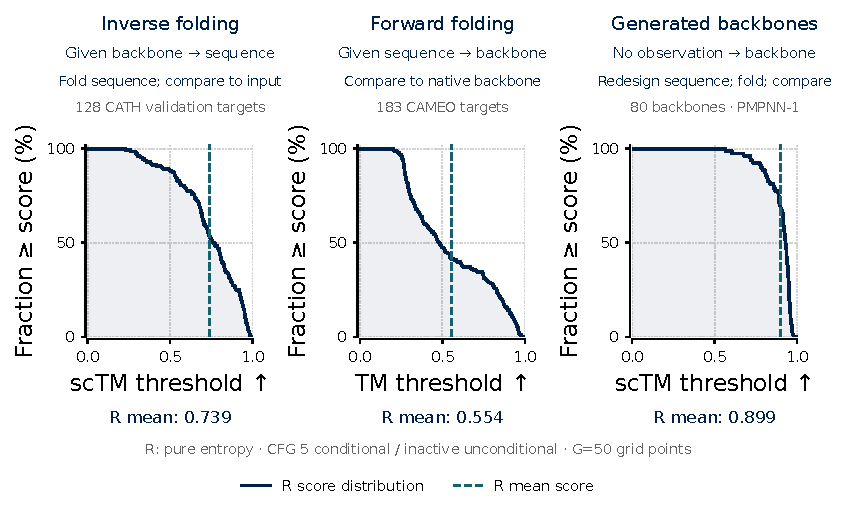
\includegraphics[width=\linewidth]{figures/protein/protein_sampler_overview.pdf}
% \caption{One checkpoint and one recipe R; no sweep maxima are shown.
% Each curve gives the fraction of targets/backbones scoring at least the horizontal
% threshold; dashed lines mark means. Left: one CoBit-sequence refold per CATH target.
% Middle: mean TM of four predictions per CAMEO target. Right: one ProteinMPNN redesign
% per generated backbone, not CoBit's own sequence. Higher curves mean more high-scoring
% examples within a task; the tasks use different references.}
% \label{fig:protein:overview}
% \end{figure}

% \begin{figure}[h!]
% \centering
% 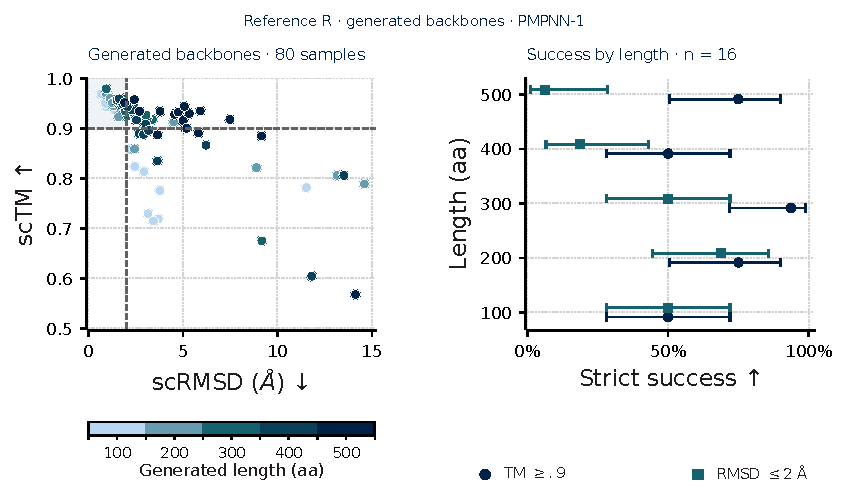
\includegraphics[width=\linewidth]{figures/protein/protein_structure_diagnostics.pdf}
% \caption{Fold similarity and coordinate accuracy are different tests.
% All 80 unconditional backbones use R and one ProteinMPNN redesign followed by ESMFold;
% these are not inverse/forward folding or CoBit-pair scores.
% Left: one dot per backbone, coloured by length; dashed lines mark scRMSD $\leq2$\,\AA{}
% and scTM $\geq.9$, and the shaded region passes both.
% Right: success fractions at each length (16 samples), with 95\% Wilson intervals.
% High TM success at long lengths does not imply low RMSD.}
% \label{fig:protein:strict}
% \end{figure}

% \begin{figure}[h!]
% \centering
% 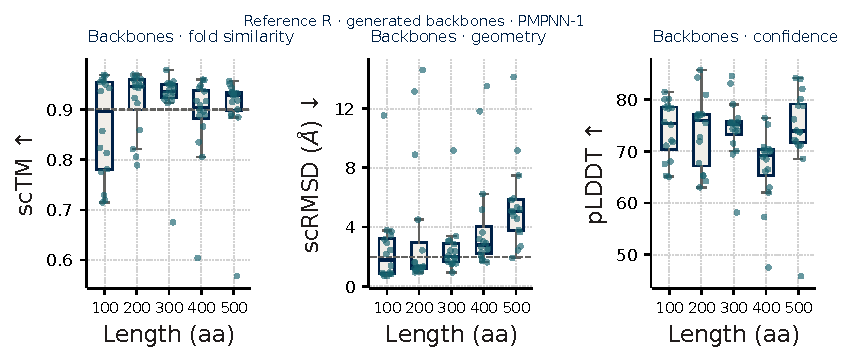
\includegraphics[width=\linewidth]{figures/protein/protein_length_distributions.pdf}
% \caption{Backbone quality across lengths 100--500 at R, using the same 80 samples
% and ProteinMPNN-1/ESMFold judge as Figure~\ref{fig:protein:strict}.
% Every dot is one backbone (16 per length); jitter only separates points.
% Boxes show medians and interquartile ranges; whiskers reach observations within
% 1.5 interquartile ranges. All outliers remain visible.
% Dashed lines mark strict TM/RMSD gates; pLDDT is predicted confidence, not experimental validation.}
% \label{fig:protein:lengthdist}
% \end{figure}

% \begin{figure}[h!]
% \centering
% 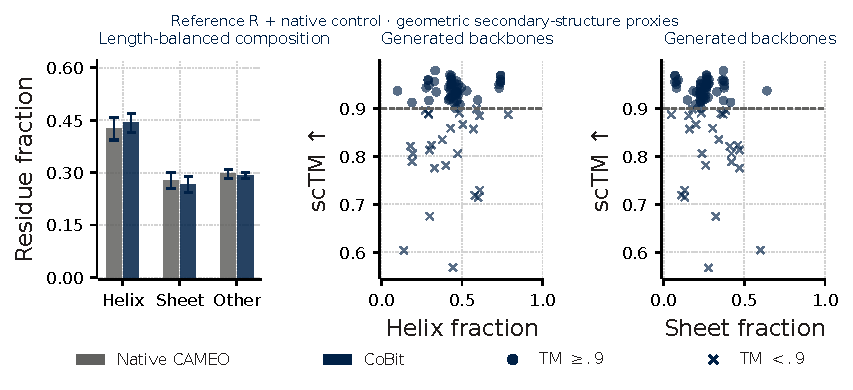
\includegraphics[width=\linewidth]{figures/protein/protein_secondary_structure.pdf}
% \caption{Coarse secondary-structure composition and backbone designability at R.
% Left: mean fractions for 80 generated backbones and 92 native CAMEO controls,
% equally weighted across five length groups; error bars are stratified 95\% bootstrap intervals.
% Middle/right: individual helix-like/sheet-like fractions versus ProteinMPNN-1 scTM;
% circles meet scTM $\geq.9$, crosses do not.
% These C$\alpha$ geometry proxies are not DSSP assignments, and the control is not the full PDB.
% Similar composition alone does not establish naturalness or function;
% details are in Appendix~\ref{app:protein:secondary}.}
% \label{fig:protein:secondary}
% \end{figure}
\endgroup


\section{Limitations}
\label{sec:limitations}

The experiments explore a limited part of the approach's potential. We train the denoisers from
scratch, without the text pretraining used by several competing speech--text systems. This may
particularly affect speech recognition and the semantic coherence of continuations, where paired
speech data must supply linguistic knowledge as well as cross-modal alignment. Text-pretrained
initialisation is therefore a promising direction, although controlled comparisons are needed to
establish its contribution. Protein-sequence pretraining may offer analogous benefits for
sequence--structure modelling.

Our models are also generally smaller than the strongest systems for the corresponding tasks,
and the training datasets provide limited coverage of the distributions we aim to model. For
example, the speech experiments rely on read speech, offering relatively narrow linguistic and
acoustic diversity. These choices restrict what the present results can establish about
performance at scale. Larger backbones and broader, higher-quality datasets are plausible routes
to improvement, but their effects need to be measured within this formulation.

Continuous modalities introduce a further dependence on pretrained tokenizers and decoders.
Information discarded during tokenisation is unavailable to the denoiser, while reconstruction
errors can persist even when codes are modelled accurately. The observed performance therefore
reflects both the bitstream model and its representation. Codec reconstruction results help
distinguish these effects, but do not by themselves explain the remaining generation errors.

\section{Discussion and conclusion}
\label{sec:discussion}
\label{sec:conclusion}

This work demonstrates that a flattened one-dimensional bitstream can serve as a common
representation for multimodal generation across three distinct forms of cross-modal
dependence. On MNIST-Sum, raw pixel bits and symbolic text bits form one learnable
joint distribution with no learned tokenizer: 97.56\% exact image$\rightarrow$text, 99.95\%
text$\rightarrow$image and 99.46\% mutually consistent joint samples. On speech and text, the same
formulation handles a strongly asymmetric, codec-backed pair, co-generating speech and text at
3.5\% cross-modal WER and UTMOS 3.77 from a model trained without text pretraining, while speech
recognition and thematic continuation remain its weakest directions. On protein sequence and
structure, one denoiser performs folding, inverse folding and joint generation of physically
coupled channels, and fold-level self-consistency is well ahead of coordinate-level precision:
68.75\% (55/80) of generated backbones reach scTM~$\geq$~0.9, against 38.75\% (31/80) at
scRMSD~$\leq$~2\,\AA. With changes largely
confined to tokenisation and layout, one continuous denoising formulation thus carries across a
controlled pair, an asymmetric pair and a physically coupled pair; within each checkpoint, joint
and conditional generation share the same weights.

The breadth of these results, obtained with modest backbones trained from scratch, supports the
feasibility of the approach. It motivates investigating how far stronger pretraining, larger
models, improved data coverage and better continuous-modality tokenizers can advance performance
while preserving the shared bitstream formulation.

% Required by the ICLR 2027 AI Policy for Authors. Does not count toward the page limit.
\subsection*{AI use statement}

In this work, we used generative AI tools, including large language model assistants, to help
implement methods (writing and editing the training, data-processing and evaluation code), to clean
and reformat datasets (building the token and bitstream caches and the scripts that compose the
MNIST-Sum pairs), and to interpret results (drafting summaries and error decompositions from
evaluation outputs, and checking reported numbers against them). Separately, a large language model
is part of the speech--text evaluation protocol: GPT-4o scores the thematic relevance of speech
continuations as an LLM-as-a-Judge (Appendix~\ref{app:audio:protocol}). We have not used generative
AI tools to generate synthetic data sets, to propose or refine hypotheses, to develop theoretical
models or conceptual frameworks, or to design or provide feedback on the research methodology or
experiments. Formulating or proving mathematical claims and translation are not applicable to this
work. Additionally, we used generative AI tools to create and edit software code, including the
scripts that produce the figures, to search for and summarise related literature, and to draft and
edit parts of the paper for readability. We have reviewed all AI-assisted work: the authors ran and
tested all AI-assisted code on their own infrastructure, checked every reported number against the
evaluation outputs, read and edited all AI-assisted text, and checked references and statements about
related work against the original papers. We take responsibility for the final content of this work,
including text, claims or artifacts produced with the aid of generative AI.


\bibliography{iclr2026_conference}
\bibliographystyle{iclr2027_conference}

\appendix
\section{Additional method details}
\label{app:method}

This appendix records implementation details inherited from text-only CoBit
\citep{method:cobit}. The main paper focuses on the multimodal representation and partial-denoising
objective used in this work.

\subsection{Continuous bitstream diffusion}

CoBit uses a variance-exploding Gaussian diffusion with, by default,
$\sigma\in[0.002,80]$ (CoBit-MLS trains with $\sigma_\text{min}=0.01$), data centre $1/2$ and $\sigma_{\mathrm{data}}=1/2$. The analytic posterior
logit of an isolated bit under a uniform prior,
$(\vx_\sigma-\tfrac12)/\sigma^2$, is clipped to $\pm30$ and added to a learned contextual
residual. The network therefore concentrates on dependencies between bits rather than relearning
the local binary denoising problem.

The entropy-derived schedule estimates the conditional entropy rate from the unweighted
per-example error, $\hat h(\sigma)\propto e(\sigma)/\sigma^2$. Estimates are stored in a FIFO buffer
of $8\times10^5$ examples and 128 log-spaced bins. The training proposal and sampling grid use
$q(\sigma)\propto g(\sigma;c,n)\hat h(\sigma)^{1/2}$, where
$g(\sigma;c,n)=\sigma^n/(\sigma^n+c^n)$ with $c=0.1$ and $n=3$. Training begins with the EDM
log-normal proposal ($P_{\mathrm{mean}}=-1.2$, $P_{\mathrm{std}}=1.2$), interpolates to $q$ over
steps $4$--$5\times10^4$ by default (CoBit-LibriTTS warms up over $1$--$1.3\times10^4$ steps), and refreshes the estimate every $2\times10^3$ steps.

For self-conditioning, the denoiser receives a second input $\hat\vx_0$. With probability
$p_{\mathrm{sc}}=0.5$, a detached no-gradient pass supplies this estimate during training;
otherwise it is zero. At inference, \texttt{carry} mode passes the previous prediction to the next
step without another evaluation; the \texttt{refined} mode, used for the protein evaluations, recomputes the estimate
at the new state and doubles the cost per step.

Sampling integrates the probability-flow ODE with a first-order DDIM/Euler step on the
entropy-derived grid, optionally with EDM-style churn \citep{method:ddim,image:edm}. Final
probabilities are thresholded at $1/2$ and regrouped into codes. The Sequence Diffusion Transformer
patches the $m$ bits at each position into one trunk token, uses RoPE, SwiGLU and adaLN-zero noise
conditioning, and combines the trunk output with the raw noisy bits in a light skip-connection
head.

\subsection{Representation and partial denoising}

Each frozen tokenizer maps its modality to integer codes and decodes predicted codes after
sampling. Per-modality vocabularies occupy disjoint ranges of one integer code space together with
padding and structural markers. The bit width $m$ covers their union, so namespace information is
part of the same binary word as token content. Markers remain clean throughout training and
sampling. Fixed token budgets are truncated or padded, and two-dimensional grids are flattened in
the order specified by the experiment.

Training draws a conditioning regime for each example. The mask $M$ marks clean conditioning bits
and the loss is evaluated only on $1-M$. When self-conditioning is active, clean conditioning bits
are also copied into $\hat\vx_0$.

% For classifier-free guidance, conditioning segments are replaced
% by the null value $1/2$ with probability $p_{\mathrm{uncond}}=0.1$ while markers remain protected.
% Examples whose conditioning was dropped are excluded from the entropy-rate buffer so that the
% estimated schedule reflects the conditional tasks.

At inference, the task fixes $M$. Conditioned positions are clamped before every denoiser call and
their ODE velocity is set to zero. Guidance combines conditional and unconditional predictions in
probability space as $D_g=D_u+w(D_c-D_u)$. The two branches are evaluated as one batch and carry
separate self-conditioning estimates. Joint generation uses one evaluation per step; guided
conditional generation uses two.

\ifdefined\toyimageonly
\section{Image and text: MNIST-Sum details}
\label{app:image}

\subsection{Protocol}
\label{app:image:mnist}

\textbf{Corpus and representation.} Each example contains four native $28{\times}28$ MNIST digits
in raster order and the corresponding equation, including its sum. We sample $10^6$ examples and
hold out 10\% of the $10^4$ possible digit tuples. Pixels are binarised and flattened digit-major,
then row-major within each digit, so every 28-bit image position is one complete digit row. Text
belongs to a closed 40-symbol language (number words 0--36, ``$+$'', ``$=$'' and padding)
represented by deterministic 7-bit codes, four per 28-bit position. The sequence has 121
positions of 28 bits (3 text, 112 image and 6 markers; 3,388 bits in total). Neither modality uses a learned tokenizer.

\textbf{Training and evaluation.} The $12{\times}512$ denoiser (63.0M parameters) trains for 500K
steps with the shared diffusion objective, entropy controller, self-conditioning and task
mixture, and receives only the flattened sequence and its 1-D position. The positional settings
are those of the speech--text models, with four local Fourier features and an intra-patch period
of $P-1$; there is no segment embedding.
Evaluation uses EMA weights, 256 steps and $n{=}4{,}096$ independently sampled examples per
direction and split. Confidence intervals are 95\% Wilson intervals.

\subsection{Results, calibration and error decomposition}

\begin{table}[h]
\centering
\small
\setlength{\tabcolsep}{6pt}
\begin{tabular}{lrrr}
\toprule
& Seen tuples & Held-out tuples & CI (seen) \\
\midrule
Image$\rightarrow$text, exact string match & 97.56 & 97.85 & $[97.04, 97.99]$ \\
Text$\rightarrow$image, all four digits & 99.95 & 99.93 & $[99.82, 99.99]$ \\
Joint from noise, mutually consistent & 99.46 & --- & $[99.19, 99.65]$ \\
\bottomrule
\end{tabular}
\caption{MNIST-Sum task accuracy (\%), $n{=}4{,}096$ per direction and split. ``Held-out'' uses digit tuples
absent from training. Joint generation is counted correct only when the generated equation is
arithmetically valid and names the four digits in the generated image.}
\label{tab:app:mnist:complete}
\end{table}

\textbf{Image$\rightarrow$text} is scored by exact string equality, without a learned instrument.
The held-out interval $[97.36, 98.25]$ overlaps the seen interval almost entirely, so the
generalisation gap is not statistically distinguishable from zero. The seen result decomposes
into 97.66\% correct perception of all four digits, 99.90\% correct arithmetic given correct
perception and no malformed output. Per slot, perception is 99.41\%, 99.12\%, 99.58\% and
99.49\% for the top-left, top-right, bottom-left and bottom-right digits. An image-blind model
that always answers the most common sum scores 6.52\% on seen tuples and 7.80\% on held-out
tuples.

\textbf{Text$\rightarrow$image} and the image half of joint generation are read by one fixed
quadrant classifier, which is correct on 99.99\% of generated quadrants. Its ceiling depends on
which pool of real digits it is shown: it identifies all four digits in 96.09\% of composites
built from the MNIST test pool, from which the validation and held-out splits are drawn, and in
99.78\% of composites built from the train pool it was itself fitted on. Generated digits
imitate the train pool, so 99.78\% is the relevant ceiling; read against the 96.09\% figure the
model would appear to exceed the instrument, which is meaningless. These are reported as
calibrations rather than used to normalise the generation score.

\textbf{Joint co-generation} samples image and text from noise in one trajectory. Of the 4,096
pairs, 100.00\% have a well-formed equation, 99.71\% name the four digits that the classifier
reads in the generated image and 99.76\% are arithmetically valid; the 99.46\% that satisfy all
three is the reported rate. Cross-modal disagreement (0.29\%) and arithmetic error (0.24\%) are
of comparable size, so the residual failures cannot be attributed mainly to either.

\else

\section{Image and text experiments}
\label{app:image}

Supporting material for \S\ref{sec:exp:imagetext}. Every figure was read from the job log of the
run that produced it. Unless stated otherwise, sampling is deterministic DDIM on the
entropy-derived grid with \texttt{carry} self-conditioning and $\sigma_{\mathrm{dec}}{=}0.1$, and
sweeps are at $n{=}5{,}000$.

\subsection{Protocol, checkpoints and the floor of the FID column}
\label{app:image:protocol}

\textbf{Zero-shot MS-COCO.} 30{,}000 captions are sampled with a fixed seed from COCO
\texttt{val2014} \citep{image:mscoco}, one image is generated per caption, and FID
\citep{image:fid} is computed with Inception-V3 pool3 features against the 30{,}000 real images
(both resized on the shorter side to 256 and centre-cropped). CLIP score is
$100\cdot\overline{\cos}(\text{image},\text{text})$ with OpenAI ViT-B/32 \citep{image:clip};
ViT-L/14 is also given in Table~\ref{tab:app:image:headline-full}, because published CLIP scores
use that backbone and the two scales differ substantially. CMMD \citep{image:cmmd} is the squared maximum mean discrepancy between the
L2-normalised CLIP ViT-B/32 embeddings of generated and real images under a Gaussian RBF kernel,
$\mathrm{CMMD}=1000\,\widehat{\mathrm{MMD}}^2_u(X_{\mathrm{gen}},X_{\mathrm{real}})$ with the
unbiased U-statistic estimator; the bandwidth $\sigma$ is the median pairwise distance of the real
bank, fixed once and reused for every configuration, and the real--real term is precomputed, so all
rows share one kernel. This departs from the reference implementation in two ways (ViT-L/14@336
embeddings and a fixed $\sigma{=}10$ there), so our CMMD values are comparable with each other but
not with CMMD figures published elsewhere. CMMD and SWD are
computed in this space against a 30{,}000-image real bank; precision and recall follow
\citet{image:precision-recall} in the same space ($k{=}3$). Captioning uses the complete Karpathy
test split (5{,}000 images) with \texttt{pycocoevalcap} including SPICE \citep{image:spice};
CLIPScore and RefCLIPScore follow \citet{image:clipscore}. GenEval \citep{image:geneval} uses the
official harness (553 prompts $\times$ 4 images). The FID reference statistics and prompt captions
are byte-identical between the $f16$ and $f8$ asset builds, and both models' image$\rightarrow$text
runs evaluate the same 5{,}000 images in the same order, so the cross-model comparisons are exact
on both sides.

\textbf{Operating points.} Classifier-free guidance evaluates the conditional and null branches as
one batch (\S\ref{sec:method:directions}), so $\mathrm{NFE}=2\times$steps for guided directions and
$=$steps for joint generation. Text$\rightarrow$image: deterministic, guidance 2.5 (CC3M) / 2.0
(CC12M), 10 / 16 steps. Image$\rightarrow$text CLIP: churn $\gamma{=}0.175$, guidance 3.0, 256
steps. Captioning: churn $\gamma{=}0.175$, guidance 2.0, 256 steps. Joint: deterministic,
unguided. Each was chosen by a bracketed sweep read on CMMD (CIDEr for captioning) and confirmed
at the full protocol where one exists. Two repeats of the 256-step headline five days apart gave
FID 22.7843 and 22.7881 (CMMD 22.1704 / 22.1627); they differ in world size, so they bound seed
and sharding variation together and the $\approx0.05$ FID threshold they set is a conservative
one.

\textbf{Sample-count bias, and the floor.} FID is strongly biased in $n$: at a fixed configuration
CC3M scores 28.10 at $n{=}5{,}000$ against 22.79 at $n{=}30{,}000$ (256 steps), and 24.00 against
18.73 at 10 steps, while CMMD moves by under one point. Sweeps are therefore read on CMMD, FID is
quoted at $n{=}30{,}000$ wherever a full-protocol run exists, and FID is never compared across
different $n$. FID at this $n$ is also bounded away from zero. A disjoint 30{,}000-image real draw
from COCO \texttt{train2014} (seed 42, zero image-id overlap; neither model trains on COCO) scores
\textbf{2.35} against the same reference, 99\% of it in the covariance term. This is the practical
disjoint-real floor for our protocol; it combines finite-sample estimation with any train/val
split shift, which this comparison alone cannot separate. The same draw after a tokenizer
round-trip gives 2.94 ($f16$) and 2.55 ($f8$), so the codec adds 0.59 and 0.20, and those are the
numbers a generative FID is read against here. The paired reconstruction FID of
Table~\ref{tab:app:image:modeldiff} (1.59 / 0.73) compares images with their own round-trip and so
omits the finite-sample term that every disjoint-set FID carries, the generative one included; it
is a codec statistic, not a quantity to subtract from a generative FID. Neither codec is
handicapped by its ImageNet training domain: on a matched 500-image comparison both reconstruct
CC3M and CC12M \emph{better} than ImageNet itself ($f8$ LPIPS 0.064 / 0.083 against 0.103, with
non-overlapping 95\% intervals).

\begin{table}[tb]
\centering
\footnotesize
\begin{tabular}{lrr}
\toprule
& \textbf{CoBit-CC3M} & \textbf{CoBit-CC12M} \\
\midrule
Training corpus & CC3M ($\approx$2.9M pairs) & CC12M ($\approx$11.7M pairs) \\
Parameters; layers $\times$ width & 462M; $24\times1024$ & 633M; $26\times1152$ \\
Image tokenizer (Open-MAGVIT2, 18-bit LFQ) & $f16$: $16{\times}16=256$ & $f8$: $32{\times}32=1{,}024$ \\
Text budget $L_t$; positions; bits $S$ & 48; 310; 5{,}890 & 96; 1{,}126; 21{,}394 \\
Training steps; relative compute & 1{,}000{,}000; $1\times$ & 1{,}744{,}000; $\approx8.7\times$ \\
\midrule
\emph{Tokenizer rFID, paired / PSNR (COCO-30K)} & 1.592 / 22.24 dB & \textbf{0.726} / \textbf{26.92 dB} \\
\emph{Codec contribution to an unpaired FID} & 0.588 & \textbf{0.199} \\
\bottomrule
\end{tabular}
\caption{The two checkpoints. CC12M has $4\times$ the data, $1.37\times$ the parameters,
$3.63\times$ the positions per step and $1.74\times$ the steps, and a materially better codec, so
every image-side comparison in \S\ref{app:image:scaling} is biased in CC12M's favour. The paired
rFID is the Fr\'echet distance between the 30{,}000 real images and their own round-trip; the row
below it is the codec's contribution when the two sets are disjoint, which is the quantity
comparable to a generative FID.}
\label{tab:app:image:modeldiff}
\end{table}

\begin{figure}[tb]
\centering
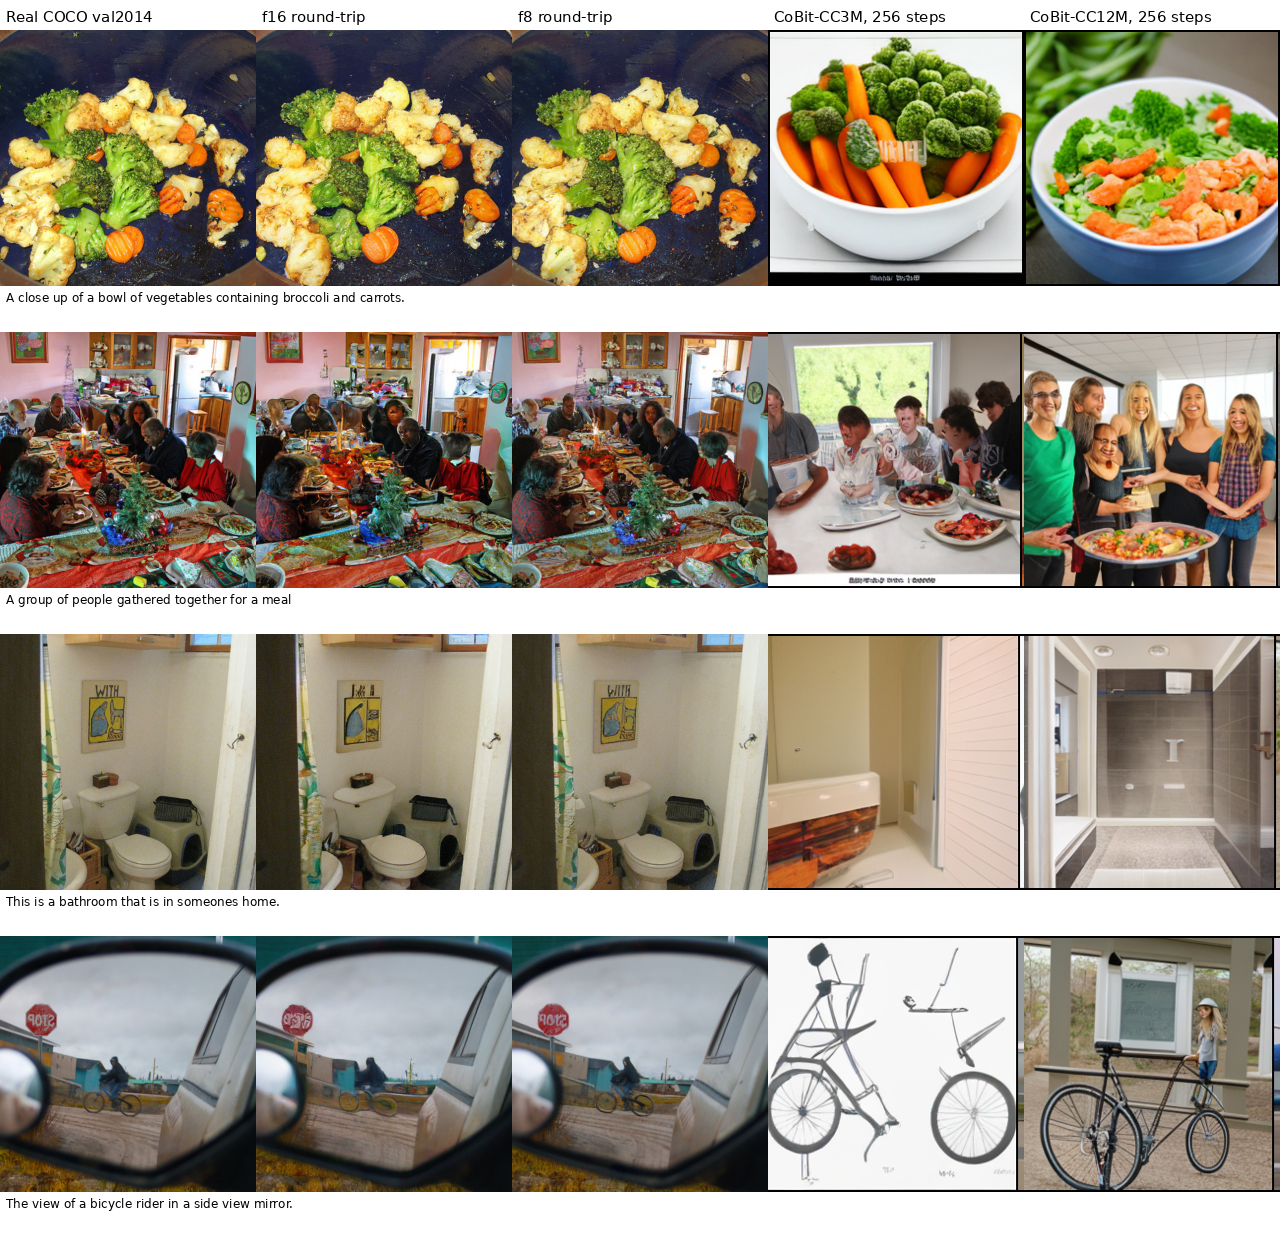
\includegraphics[width=\linewidth]{figures/image_text/real_recon_generation.png}
\caption{Where the gap is. Left to right: a real MS-COCO \texttt{val2014} image, its round-trip
through the frozen $f16$ and $f8$ Open-MAGVIT2 codecs, and text$\rightarrow$image samples from
CoBit-CC3M and CoBit-CC12M for that image's own caption, at 256 steps. The two round-trip columns
are hard to tell from the real image, consistent with a measured codec contribution of 0.59 / 0.20
FID over a 2.35 disjoint-real floor; the visible distance is between the round-trips and the
generations. The first four of seven fixed-protocol captions, one uncurated sample each,
illustrating the measured floors of \S\ref{app:image:protocol} rather than standing in for them.}
\label{fig:image:gap}
\end{figure}

\subsection{Complete results}
\label{app:image:headline-full}

\begin{table}[tb]
\centering
\footnotesize
\setlength{\tabcolsep}{3.5pt}
\begin{tabular}{llrrrrrrrrr}
\toprule
\textbf{Direction} & $n$ & gs & Steps & \textbf{FID}$\downarrow$ & \textbf{CMMD}$\downarrow$ & \textbf{SWD}$\downarrow$
& \multicolumn{2}{c}{\textbf{CLIP}$\uparrow$} & \textbf{Prec.} & \textbf{Rec.} \\
\cmidrule(lr){8-9}
& & & & & & & B/32 & L/14 & & \\
\midrule
\multicolumn{11}{l}{\emph{CoBit-CC3M}}\\
text $\rightarrow$ image & 30{,}000 & 2.5 & 10 & \textbf{18.48} & \textbf{18.41} & 0.632 & 27.73 & --- & --- & --- \\
text $\rightarrow$ image & 30{,}000 & 3.0 & 10 & 18.73 & 18.56 & 0.631 & 28.03 & 21.66 & 0.48 & 0.28 \\
text $\rightarrow$ image & 30{,}000 & 3.0 & 256 & 22.79 & 22.16 & 0.667 & 28.02 & 21.79 & 0.41 & 0.29 \\
image $\rightarrow$ text & 10{,}000 & 3.0 & 256 & --- & --- & --- & 24.86 & 18.30 & --- & --- \\
image $\rightarrow$ text & 10{,}000 & 4.0 & 256 & --- & --- & --- & 24.99 & --- & --- & --- \\
joint (unconditional) & 30{,}000 & --- & 10 & 50.19 & 41.53 & 0.904 & 23.10 & 16.87 & 0.36 & 0.22 \\
joint (unconditional) & 30{,}000 & --- & 256 & 61.95 & 46.80 & 0.971 & 25.67 & --- & 0.20 & 0.30 \\
\midrule
\multicolumn{11}{l}{\emph{CoBit-CC12M}}\\
text $\rightarrow$ image & 30{,}000 & 2.0 & 16 & \textbf{16.59} & 17.76 & 0.591 & 26.51 & --- & --- & --- \\
text $\rightarrow$ image & 30{,}000 & 2.0 & 20 & 16.70 & \textbf{17.68} & 0.585 & 26.54 & --- & --- & --- \\
image $\rightarrow$ text & 5{,}000 & 4.0 & 256 & --- & --- & --- & 23.08 & --- & --- & --- \\
joint (unconditional) & 5{,}000 & --- & 20 & 56.18 & 37.60 & 0.837 & 23.19 & --- & --- & --- \\
joint (unconditional) & 5{,}000 & --- & 256 & 64.47 & 40.33 & 0.878 & 24.01 & --- & --- & --- \\
\bottomrule
\end{tabular}
\caption{Full version of Table~\ref{tab:image:headline}; the CLIP column of the joint rows is pair
coherence. L/14, precision and recall were measured at guidance 3.0 only. Moving CC3M from 256 to
10 steps raises precision $0.41\rightarrow0.48$ with recall $0.29\rightarrow0.28$, so the gain is
not a diversity-for-fidelity trade. Only the L/14 column is comparable with published CLIP scores:
UniDiffuser \citep{image:unidiffuser} reports roughly 25--26 and 22 on the two directions against
our 21.66--21.79 and 18.30, consistent with the FID gap and its LAION-scale pre-training.}
\label{tab:app:image:headline-full}
\end{table}

\subsection{Sampler characterisation}
\label{app:image:sampler}

\begin{table}[tb]
\centering
\footnotesize
\setlength{\tabcolsep}{5pt}
\begin{tabular}{rrrr@{\hspace{10pt}}rr@{\hspace{10pt}}rr}
\toprule
& \multicolumn{3}{c}{text $\rightarrow$ image} & \multicolumn{2}{c}{joint} & \multicolumn{2}{c}{text-emitting} \\
\cmidrule(lr){2-4}\cmidrule(lr){5-6}\cmidrule(lr){7-8}
Steps & FID$\downarrow$ & CMMD$\downarrow$ & CLIP$\uparrow$ & FID$\downarrow$ & pair-CLIP$\uparrow$ & CIDEr$\uparrow$ & i2t CLIP$\uparrow$ \\
\midrule
4   & 28.54 & 22.71 & 27.45 & --- & --- & --- & --- \\
6   & 24.79 & 19.13 & 27.86 & --- & --- & --- & --- \\
8   & 24.28 & 18.81 & 27.99 & --- & --- & --- & --- \\
\textbf{10}  & \textbf{24.00} & \textbf{18.76} & 28.04 & \textbf{56.06} & 23.16 & 0.0131 & 23.91 \\
12  & 24.03 & 18.95 & 28.05 & --- & --- & --- & --- \\
16  & 24.68 & 19.40 & 28.05 & --- & --- & --- & --- \\
32  & 26.13 & 20.85 & 28.03 & 59.14 & 24.71 & 0.0588 & 24.34 \\
64  & 27.21 & 21.59 & 28.00 & 62.66 & 25.17 & 0.0488 & 24.53 \\
128 & 27.79 & 22.18 & 27.96 & --- & --- & 0.1304 & --- \\
\textbf{256} & 28.10 & 22.57 & 28.00 & --- & --- & \textbf{0.1362} & 24.83 \\
512 & --- & --- & --- & --- & --- & 0.1032 & \textbf{24.90} \\
\bottomrule
\end{tabular}
\caption{CoBit-CC3M, every direction against the step count, $n{=}5{,}000$. The asymmetry is the
whole point: text$\rightarrow$image minimises at 10 in a bowl bracketed on both sides (8--14) and
climbs monotonically above it, captioning peaks at 256 and keeps a tenth of its CIDEr at 10, and
the joint direction moves both ways at once because both halves come from one trajectory. The CLIP
column is flat to within 0.1 from 8 steps on and cannot see the 4.1-point FID swing beside it; the
64-step CIDEr falling below 32 puts run-to-run noise near 0.01. Text$\rightarrow$image is at
guidance 3.0, captioning at 2.0 with churn $\gamma{=}0.175$, image$\rightarrow$text at 3.0; guided
directions cost $\mathrm{NFE}=2\times$steps, joint $1\times$. At the full protocol
($n{=}30{,}000$) CC3M moves from FID 22.79 at 256 steps to 18.73 at 10, $-4.06$ at $1/25.6$ the
cost. CC12M behaves the same way at guidance 2.0, optimum 16--20: FID 24.97 / 22.21 / \textbf{21.68} /
21.96 / 22.22 / 22.81 / 23.58 / 27.22 at 8 / 12 / 16 / 20 / 24 / 32 / 48 / 256 steps, a larger gain
over 256 steps ($-5.54$) than CC3M's $-4.10$ on the same $n$.}
\label{tab:app:image:steps}
\end{table}

\paragraph{Guidance.} CMMD minimises near guidance 2 for both models (CC3M 25.80 / 23.10 /
\textbf{22.44} / 22.57 / 22.71 / 23.27 at guidance 1.0 / 1.5 / 2.0 / 3.0 / 4.0 / 5.0, 256 steps;
CC12M 22.32 / 21.39 / \textbf{21.25} / 22.32 / 23.24 at 1.0--4.0), FID one to two notches higher,
and CLIP rises monotonically throughout, so past the peak image quality must be judged on CMMD
rather than CLIP. Both optima are bracketed on both sides. Guidance and step count are close to
separable: re-sweeping at the re-tuned step counts leaves the structure unchanged (CC3M at 10
steps, guidance 2.0 / 2.5 / 3.0: CMMD 18.77 / \textbf{18.50} / 18.76; CC12M at 20 steps, guidance
1.5 / 2.0 / 2.5 / 3.0: 18.70 / \textbf{17.79} / 17.92 / 18.33), which is why the one-dimensional
step sweep at fixed guidance was a valid search. CC12M loses CLIP to CC3M at every matched
guidance value (by 0.52--1.02) while winning FID and CMMD at guidance 1--3.

\paragraph{Churn, schedule, self-conditioning.} Measured on CC3M at 256 steps, hence far from the
image optimum. \emph{Churn} is strongly harmful for text$\rightarrow$image---at guidance 3.0, FID
28.10 / CMMD 22.57 deterministic against 36.89 / 34.73 at $\gamma{=}0.1$ and 41.87 / 40.51 at
$\gamma{=}0.175$, while CLIP moves by at most 0.06---yet the same $\gamma{=}0.175$ is what makes
captioning work at all (deterministic decoding is degenerate, CIDEr 0.018). \emph{Schedule}: for
text$\rightarrow$image the entropy-derived and Karras grids agree at the guidance values actually
used, 0.03--0.14 FID apart at guidance 3--5, and separate below them, reaching 0.82 FID in
Karras's favour at guidance 1.0; the two arms ran two days apart on code that logged no sampler
configuration, so we do not read that gap either way. For captioning the entropy-derived grid is
decisively better, CIDEr 0.136 versus 0.049 at guidance 2.0, so a text$\rightarrow$image-only
ablation would have concluded the schedule does not matter. \emph{Self-conditioning}:
\texttt{carry} matches \texttt{refined} at guidance 3.0 (CMMD 22.30 versus 22.44, CLIP 27.98
versus 27.99, both at $n{=}2{,}000$) at half the NFE, so \texttt{carry} is used throughout.

\paragraph{What the semantic metrics cannot see.} Four results say the same thing. The CLIP column
of Table~\ref{tab:app:image:steps} is flat to within 0.1 between 8 and 256 steps; the CLIP of the
guidance paragraph above keeps rising past the point where CMMD and FID have turned; under churn
CLIP moves by 0.06 while FID moves by 13.8; and GenEval is step-invariant
(\S\ref{app:image:geneval}). The embedding and compositional metrics cannot resolve image-quality
differences that the distributional ones register clearly. Which family better tracks human
preference we do not test here; settling it needs a preference model over hundreds of samples, not
inspection of a grid.

\subsection{CC3M versus CC12M}
\label{app:image:scaling}

\begin{table}[tb]
\centering
\small
\begin{tabular}{lrrl}
\toprule
& \textbf{CC3M} & \textbf{CC12M} & $\Delta$ \\
\midrule
\multicolumn{4}{l}{\emph{Text$\rightarrow$image at each model's own optimum, $n{=}30{,}000$}}\\
operating point & 10 steps, gs 2.5 & 16 steps, gs 2.0 & \\
\textbf{FID} (raw) $\downarrow$ & 18.48 & \textbf{16.59} & $-1.89$ \\
\quad less the codec's contribution (0.59 / 0.20) & 17.90 & \textbf{16.39} & $\mathbf{-1.50}$ \\
\textbf{CMMD} $\downarrow$ / \textbf{SWD} $\downarrow$ & 18.41 / 0.632 & \textbf{17.76} / \textbf{0.591} & $-0.65$ / $-0.041$ \\
CLIP B/32 $\uparrow$ & \textbf{27.73} & 26.51 & $-1.22$ \emph{(worse)} \\
\midrule
\multicolumn{4}{l}{\emph{Text-emitting directions, matched 256 steps, $n{=}5{,}000$}}\\
captioning CIDEr / SPICE $\uparrow$ & \textbf{0.1362} / \textbf{0.0541} & 0.0571 / 0.0347 & $2.4\times$ / $1.6\times$ \emph{worse} \\
i2t CLIP B/32, gs 3.0 / 4.0 $\uparrow$ & \textbf{24.83} / \textbf{24.97} & 22.98 / 23.08 & $-1.85$ / $-1.89$ \\
GenEval overall $\uparrow$ & \textbf{0.249} & 0.222 & $-0.027$ \\
\bottomrule
\end{tabular}
\caption{Scaling verdict at each model's own optimum. CC12M wins every image-side
\emph{distributional} metric and loses CLIP; the CLIP row compares different guidance values
(2.5 versus 2.0), see Table~\ref{tab:app:image:matched-clip} for the matched comparison. The margin survives floor correction: the shared 2.35 sampling floor cancels and removing each
tokenizer's codec contribution leaves CC12M 1.50 ahead, so the codec explains about a fifth of the
raw gap (Fr\'echet distances are not additive, so this is a reporting heuristic for the order of
the confound; no reconstruction-CMMD floor exists, so that margin keeps an unquantified codec
advantage). The gap widens towards the optimum: at a matched guidance 2.0 and $n{=}5{,}000$ it is 3.27 FID at
32 steps against 1.39 at 256. On the text side CC3M wins everything by margins far outside the $\sim$0.01 CIDEr noise; the
candidate causes are discussed below.}
\label{tab:app:image:scaling-verdict}
\end{table}

\begin{table}[tb]
\centering
\small
\setlength{\tabcolsep}{5pt}
\begin{tabular}{llrrr}
\toprule
\textbf{Direction, setting} & \textbf{Guidance $w$} & \textbf{CC3M} & \textbf{CC12M} & $\Delta$ \\
\midrule
text$\rightarrow$image, 256 steps & 1.0 & 25.32 & 24.80 & $-0.52$ \\
 & 2.0 & 27.19 & 26.45 & $-0.74$ \\
 & 3.0 & 28.00 & 27.10 & $-0.90$ \\
 & 4.0 & 28.44 & 27.42 & $-1.02$ \\
text$\rightarrow$image, near-optimal steps (10 / 20) & 2.0 & 27.28 & 26.54 & $-0.74$ \\
 & 2.5 & 27.73 & 26.92 & $-0.81$ \\
 & 3.0 & 28.04 & 27.14 & $-0.90$ \\
\midrule
image$\rightarrow$text, 256 steps, $\gamma{=}0.175$ & 3.0 & 24.83 & 22.98 & $-1.85$ \\
 & 4.0 & 24.97 & 23.08 & $-1.89$ \\
captioning run (Karpathy test), 256 steps, $\gamma{=}0.175$ & 2.0 & 24.49 & 22.47 & $-2.02$ \\
\bottomrule
\end{tabular}
\caption{CLIP (ViT-B/32, $100\cdot\cos$) at matched guidance, $n{=}5{,}000$. CLIP rises
monotonically with $w$ for both models in every direction, so the headline values of
Table~\ref{tab:image:headline}, read at each model's CMMD optimum ($w{=}2.5$ for CC3M, $2.0$ for
CC12M), mix a guidance effect of roughly 0.4 into the 1.22-point gap. At equal guidance the gap is
0.5--1.0 for text$\rightarrow$image and 1.85--2.0 for the text-emitting directions, and it widens
with $w$. ViT-L/14 gives the same ordering (21.31 versus 20.63 at the headline points). Only
$w{=}3.0$ and $4.0$ were run for image$\rightarrow$text and only $w{=}2.0$ for captioning of both
models, so ``every tested guidance'' means these values.}
\label{tab:app:image:matched-clip}
\end{table}

\textbf{Why CC12M loses alignment while winning image quality.} Every metric that compares an image
with a text (CLIP in both directions, CIDEr, SPICE, RefCLIPScore, GenEval) moves against CC12M,
while every metric that compares an image distribution with an image distribution (FID, CMMD, SWD,
precision) moves for it (Tables~\ref{tab:app:image:scaling-verdict}
and~\ref{tab:app:image:matched-clip}). Two explanations are consistent with this pattern and the
present runs do not separate them. \emph{Data.} CC12M alt-text is longer, noisier and less literal
than CC3M's; the corpus supplies $4\times$ the images for the image prior but a looser image--text
coupling. \emph{Token budget.} The $f8$ codec quadruples the image segment (1{,}024 tokens against
256) while the text budget only doubles (96 against 48), so text is 8\% of a CC12M sequence against
16\% of a CC3M sequence. Under one modality-agnostic loss this halves the text share of the training
signal in joint examples, and in text$\rightarrow$image it halves the fraction of the context that
carries the condition; both push in the observed direction. The clean separations are a CC3M model at $f8$ (same captions, four times the
image tokens) and a CC12M model trained on CC3M-style re-captions (same tokens, cleaner text);
neither has been run.

\textbf{CLIP ceilings.} Every CLIP value above is relative: the score a real, correctly paired
image--caption has under the same preprocessing bounds what a model can reach, and it differs
between COCO (short literal captions) and the alt-text corpora the models were trained on. We
have not yet measured these ceilings and therefore do not quote absolute ratios.
\note{To measure before submission. (i) COCO: \texttt{scripts/multimodal/coco\_clip\_ceiling.py}
embeds the reference captions of the 30{,}000 bank images (no generation, no images to load; the
bank already holds the real-image embeddings under the protocol preprocessing) and reports the
mean-over-references and best-of-references real-pair CLIP for ViT-B/32 and, with the L/14 bank,
ViT-L/14, plus the same on the image$\rightarrow$text 5K subset. (ii) CC3M / CC12M validation:
the \texttt{clip\_diag} rows (\texttt{clip\_t\_gt}, \texttt{clip\_align\_gt}) in
\texttt{runs/multimodal/<exp>/evaluation\_*/results.csv}, aggregated by
\texttt{aggregate\_clip\_diag.py}. Then report each model's text$\rightarrow$image and
image$\rightarrow$text CLIP as a fraction of the COCO ceiling and of its own corpus ceiling.}


\subsection{GenEval breakdown}
\label{app:image:geneval}

\begin{table}[tb]
\centering
\small
\begin{tabular}{lrrrrrrrr}
\toprule
\textbf{Model} & \textbf{Params} & Single & Two & Count & Colors & Pos. & Attr. & \textbf{Overall} \\
\midrule
Show-o \citep{image:showo} & 1.3B & 0.98 & 0.80 & 0.66 & 0.84 & 0.31 & 0.50 & 0.68 \\
SD3 & 2B & 0.98 & 0.74 & 0.63 & 0.67 & 0.34 & 0.36 & 0.62 \\
SD v1.5 & --- & 0.97 & 0.38 & 0.35 & 0.76 & 0.04 & 0.06 & 0.43 \\
LlamaGen & 0.8B & 0.71 & 0.34 & 0.21 & 0.58 & 0.07 & 0.04 & 0.32 \\
CoBit-CC3M (ours) & 462M & 0.80 & 0.12 & 0.05 & 0.46 & 0.04 & 0.03 & 0.249 \\
minDALL$\cdot$E & --- & 0.73 & 0.11 & 0.12 & 0.37 & 0.02 & 0.01 & 0.23 \\
CoBit-CC12M (ours) & 633M & 0.68 & 0.11 & 0.06 & 0.45 & 0.01 & 0.01 & 0.222 \\
\bottomrule
\end{tabular}
\caption{Per-task GenEval; prior work as printed in \citet{image:geneval} (Table 2) and
\citet{image:showo} (Table 3). Our rows use the entropy-derived grid, deterministic sampling,
guidance 3.0 and 256 steps. The score is flat in the step count: CC3M scores 0.240 at 10 steps against
0.249 at 256 on one execution path at fixed guidance, so only the step count varies there, and
CC12M 0.221 at 16 steps against 0.222 at 256 (guidance 2.0 and 3.0 respectively). GenEval
therefore moves by under 0.01 over a range on which FID moves by 4.06.
Single objects render 80\% of the time and colours 46\% while compositional binding stays near the
floor, as it does for every sub-billion-parameter model here; CC3M alt-text rarely specifies
spatial relations or colour--object bindings. The sampler configuration matters materially: an
earlier pass of the same checkpoint that had silently fallen back to a Karras grid, at guidance
2.0, scored 0.209.}
\label{tab:app:image:geneval}
\end{table}

\subsection{Captioning}
\label{app:image:captioning}

\begin{table}[tb]
\centering
\footnotesize
\setlength{\tabcolsep}{4pt}
\begin{tabular}{lrrrrrrr}
\toprule
\textbf{Configuration} & BLEU-4 & METEOR & ROUGE-L & \textbf{CIDEr} & SPICE & CLIPScore & RefCLIPScore \\
\midrule
deterministic, gs 1.0 \emph{(degenerate)} & 0.004 & 0.054 & 0.157 & 0.018 & 0.012 & --- & --- \\
entropic, churn $\gamma{=}0.175$, gs 2.0 & \textbf{0.0291} & \textbf{0.0975} & \textbf{0.2212} & \textbf{0.1362} & \textbf{0.0541} & 0.612 & 0.6606 \\
entropic, churn $\gamma{=}0.175$, gs 4.0 & 0.0147 & 0.0695 & 0.1804 & 0.0520 & 0.0247 & \textbf{0.623} & \textbf{0.6678} \\
Karras, churn $\gamma{=}0.175$, gs 2.0 & 0.0131 & 0.0672 & 0.1792 & 0.0485 & 0.0232 & --- & 0.6578 \\
\bottomrule
\end{tabular}
\caption{CoBit-CC3M zero-shot captioning on the complete Karpathy test split ($n{=}5{,}000$, 256
steps, no empty captions). Guidance 2.0 maximises the $n$-gram metrics and guidance 4.0 the
CLIP-space metrics; the two families disagree, so both are reported. The entropy-derived grid
beats Karras by $2.81\times$ on CIDEr while RefCLIPScore moves by 0.003. CC12M's row is in
Table~\ref{tab:app:image:scaling-verdict}, where the comparison is the point.}
\label{tab:app:image:captioning}
\end{table}

\begin{figure}[tb]
\centering
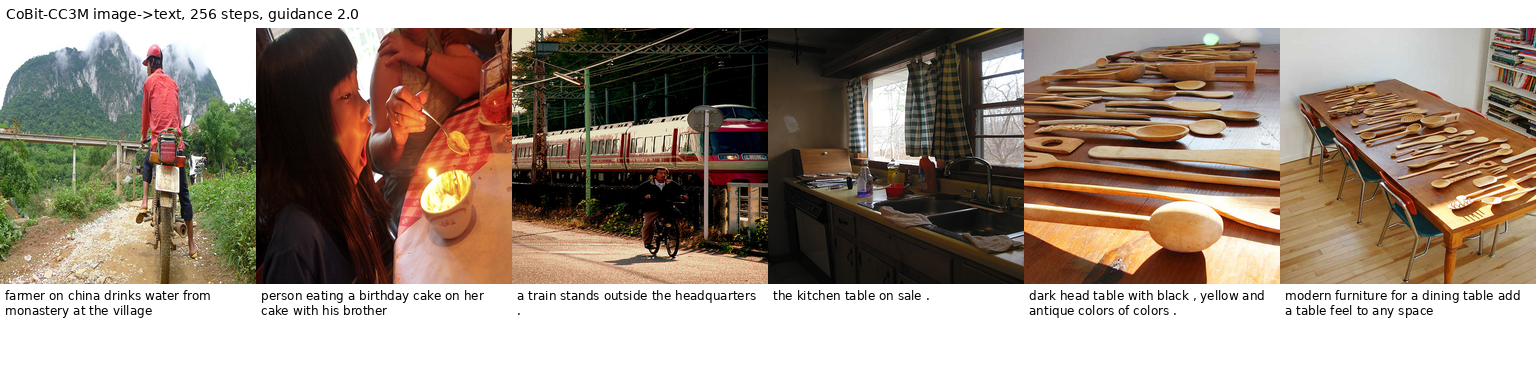
\includegraphics[width=\linewidth]{figures/image_text/cc3m_i2t_s256_gs2.0.png}
\caption{Six uncurated CoBit-CC3M image$\rightarrow$text samples at the operating point of
Table~\ref{tab:app:image:captioning}. They illustrate both semantic errors and a register mismatch:
outputs often resemble CC3M web alt-text or sales copy, whereas COCO references are terse
declaratives. CIDEr and RefCLIPScore measure different aspects of this mismatch over all 5{,}000
images; the six examples show failure types, not their prevalence.}
\label{fig:image:i2t}
\end{figure}

\textbf{No published zero-shot baseline exists for this number.} UniDiffuser
\citep{image:unidiffuser} evaluates image$\rightarrow$text with CLIP score only, and L-Verse's
captioning numbers \citep{image:lverse} are for a model trained on the MS-COCO Karpathy splits.
For scale, on the $\times100$ convention those papers use, L-Verse reaches CIDEr 102.2, $M^2$
Transformer \citep{image:m2transformer} 131.2 and OSCAR$_L$ \citep{image:oscar} 140.0, all trained
on MS-COCO; our 0.136 is roughly $7.5\times$ below L-Verse, not $100\times$. L-Verse's own
no-truncation variant moves CIDEr from 102.2 to 181.6 while BLEU-4 falls from 39.9 to 27.6 on the
same model and images, so caption length and phrasing alone swing these metrics by tens of points.
That is the failure here (Figure~\ref{fig:image:i2t}): CIDEr's IDF-weighted $n$-grams penalise the
register mismatch almost regardless of content. We report CIDEr for completeness and read the
result through RefCLIPScore.

\subsection{MNIST-Sum}
\label{app:image:mnist}

\textbf{Protocol.} Each example contains four native $28{\times}28$ MNIST digits in raster order
and the corresponding equation, including its sum. We sample $10^6$ examples and hold out 10\% of
the $10^4$ digit tuples. Pixels are binarised and flattened digit-major, then row-major within each
digit, so every 28-bit image position is one complete digit row; text belongs to a closed
40-symbol language (number words 0--36, ``$+$'', ``$=$'' and padding) represented by deterministic
7-bit codes, four per position. The sequence has 121 positions of 28 bits (3 text, 112 image and 6 markers; 3,388 bits in total).
The $12{\times}512$ denoiser (63.0M parameters) trains for 500K steps with the shared diffusion
objective, entropy controller, self-conditioning and regime probabilities, and receives only the
flattened sequence and its 1-D position. The positional settings are those of the speech--text
models (four local Fourier features, intra-patch period $P-1$) and there is no segment embedding;
these are shared positional and budget choices, not modality-specific embeddings, towers, heads or losses.
Evaluation uses EMA weights, 256 steps and $n{=}4{,}096$ samples per direction and split;
intervals are 95\% Wilson.

\textbf{Image$\rightarrow$text} is scored by exact string equality with no learned instrument:
97.56\% on seen tuples (CI $[97.04, 97.99]$) and 97.85\% on held-out tuples (CI
$[97.36, 98.25]$), so the generalisation gap is not statistically distinguishable from zero. The
seen result decomposes into 97.66\% correct perception, 99.90\% correct arithmetic given correct
perception and no malformed output.

\textbf{Text$\rightarrow$image} places all four requested digits correctly in 99.95\% of seen
samples (CI $[99.82, 99.99]$) and 99.93\% of held-out samples. This direction is read by a fixed
quadrant classifier, correct on 99.99\% of generated quadrants. Its ceiling depends on the pool of
real digits it is shown: all four digits in 96.09\% of composites built from the MNIST test pool,
from which the evaluation splits are drawn, and 99.78\% of composites built from the train pool it
was fitted on. Generated digits imitate the train pool, so 99.78\% is the relevant ceiling; these
are instrument calibrations rather than normalisation factors.

\textbf{Joint co-generation} from noise is 99.46\% mutually consistent (CI $[99.19, 99.65]$). Of
the 4,096 pairs, 100.00\% have a well-formed equation, 99.71\% name the digits the classifier reads
in the generated image and 99.76\% are arithmetically valid. Cross-modal disagreement (0.29\%) and
arithmetic error (0.24\%) are of comparable size, so the residual failures cannot be attributed
mainly to either.

\subsection{Comparability and measurement hygiene}
\label{app:image:repro}

\begin{table}[t]
\centering
\small
\setlength{\tabcolsep}{4pt}
\begin{tabular}{lrrrr}
\toprule
\textbf{Model} & \textbf{Params} & \textbf{Pre-train pairs} & \textbf{FID-30K}$\downarrow$ & \textbf{GenEval}$\uparrow$ \\
\midrule
\multicolumn{5}{l}{\emph{CoBit (ours; denoiser trained from scratch, frozen image codec)}}\\
CoBit-CC3M & 462M & 2.9M & 18.48 & 0.249 \\
CoBit-CC12M & 633M & 11.7M & 16.59 & 0.222 \\
\midrule
\multicolumn{5}{l}{\emph{Same pre-training corpus (CC3M), zero-shot COCO}}\\
LAFITE \citep{image:lafite} & 75M ($+$CLIP) & 3.3M & 26.94 & --- \\
\midrule
\multicolumn{5}{l}{\emph{Unified image$+$text models}}\\
CoDI \citep{image:codi} & --- & 400M & 22.26 & 0.31 \\
SEED-X \citep{image:seedx} & 17B & --- & 14.99 & 0.49 \\
LWM \citep{image:lwm} & 7B & --- & 12.68 & 0.47 \\
UniDiffuser \citep{image:unidiffuser} & 952M & LAION-5B (subsets) & 9.71$^{\dagger}$ & --- \\
Show-o \citep{image:showo} & 1.3B & 35M & 9.24 & 0.68 \\
\midrule
\multicolumn{5}{l}{\emph{Text-to-image specialists}}\\
DALL$\cdot$E \citep{image:dalle} & 12B & 250M & 27.50 & --- \\
LDM \citep{image:ldm} & 1.4B & 400M & 12.63 & 0.37 \\
SD v1.5 \citep{image:ldm} & 0.9B & 2000M & 9.62 & 0.43 \\
PixArt-$\alpha$ \citep{image:pixart} & 0.6B & 25M & 7.32 & 0.48 \\
\bottomrule
\end{tabular}
\caption{Zero-shot MS-COCO FID-30K and GenEval as reported by each source. The rows provide scale
context rather than a ranking: data, parameter counting and evaluation implementations differ.
$^{\dagger}$UniDiffuser does not identify which sample count belongs to FID.}
\label{tab:image:litcomparison}
\end{table}

\textbf{Literature figures.} Every number in Table~\ref{tab:image:litcomparison} was read from the
cited paper's own table or from the compilation tables of \citet{image:showo},
\citet{image:unidiffuser} and \citet{image:lafite}. Improved VQ-Diffusion
\citep{image:vqdiffusion-improved}, our closest architectural relative, is excluded because
neither of its figures (FID 8.44 on MS-COCO, 15.58 on Conceptual Captions) is a zero-shot COCO
number; CogView \citep{image:cogview} is excluded because its 27.10 blurs MS-COCO, translates the
captions into Chinese and re-ranks 60 samples per caption. Three conventions flatter different
rows. \emph{Parameters} are as each source counts them and frozen components are included
inconsistently: PixArt-$\alpha$'s 0.6B excludes a 4.3B T5 encoder and LAFITE's 75M counts only
trainable weights, while other sources fold a frozen encoder into the figure they print.
DALL$\cdot$E's 27.50 is itself a best-of-512 CLIP-reranked number that its own paper does not
print; we reproduce it as the compilations give it. Four further rows---minDALL$\cdot$E, LlamaGen,
DALL$\cdot$E~2 and Imagen---are left out of Table~\ref{tab:image:litcomparison} for space; the
first two appear in Table~\ref{tab:app:image:geneval}, and the others report FID 10.39
\citep{image:dalle2} and 7.27 \citep{image:imagen}.
\emph{Pre-train pairs} count different things, and CC3M is 3.3M pairs as released against the 2.9M
still downloadable when we built it, which is why the LAFITE and CoBit-CC3M rows differ on a
shared corpus. \emph{FID} is not one pipeline: Stable Diffusion is 8.59 in one compilation and
9.62 in another, the same model measured twice, which sets the scale on which small differences
should be read. Separately, our generations reproduce CC3M's distribution---stock-photo
watermarks, white backgrounds, single subjects---against COCO's multi-object scenes, and that
distance penalises FID independently of image quality.

\textbf{Schedule audit.} If the entropy tables are absent from a run directory the sampler
silently reverts to a Karras grid. Every run was audited for the corresponding warning and every
number reported here comes from a run with a count of zero; where the fallback did occur, the run
either supplies a ``Karras'' arm of a schedule comparison, in which the fallback is the treatment,
or was superseded by a fallback-free repeat whose numbers are the ones printed. The audit is not
optional: the unaudited GenEval pass that scored 0.209 had fallen back. Separately, CC3M's GenEval
0.249 was produced on the eager execution path, which is the path on which a bf16 defect
invalidated an earlier set of CC12M scores; it is unaffected, on two controlled pairs---eager
versus compiled at 10 steps (0.240 versus 0.235) and 10 versus 256 steps on the eager path (0.240
versus 0.249)---because CC3M's 256-token sequence does not trigger it.

\fi

\section{Audio and text experiments}
\label{app:audio}

\subsection{Protocol and Checkpoints} \label{app:audio:protocol}

\textbf{LibriVox-based corpora.} LibriTTS, MLS-English, LibriSpeech-PC and part of SALMON (background and room partitions) are extracted from the LibriVox project, and thus consist of single-speaker, reading-style audiobook recordings. The content CoBit sees during training is exclusively story passages, which severely constrains its stylistic and thematic exposure. Availability of in-the-wild text-audio pairs is very limited at this scale for single-speaker samples, so audiobook data is the natural alternative. For most speech models, semantic and stylistic generality is inherited from the text pre-trained backbone. Note that the training and test sets have no example or speaker overlap. 

\textbf{Linguistic evaluation.} To assess the linguistic properties of generated speech signals, we transcribe them using an external Whisper-large \citep{audio:whisper} ASR model. For co-generation, error rates are computed between the two generated sequences. The fluency of a text sequence is measured by its perplexity under an external language model (in this case Llama-3.2 1B), computed separately for each modality in co-generation and for speech transcriptions in speech continuation. To further determine the conceptual relevance of produced continuations, \texttt{GPT-4o} is employed in an LLM-as-a-Judge setting, assigning each continuation a score from 1 to 5. The system message is taken directly from \cite{audio:taste} and presented in Table \ref{tab:audio:llm-judge}.

\begin{table}[t]
\centering
\small
\setlength{\tabcolsep}{4.5pt}
\begin{tabular}{l}
\toprule
The task is evaluating the relevance and likelihood of the predicted text continuation, given the text prompt. \\ 
You should also consider whether the meaning of the text continuation is making sense. \\
The text prompt is: "\texttt{prompt}", and the text continuation is: "\texttt{content}" \\ \\

You must give an overall rating from 1 to 5. The rating guideline is as below: \\
1: The text continuation is very unlikely and irrelevant to the text prompt. \\
2: The text continuation is unlikely and marginally relevant to the text prompt. \\
3: The text continuation is moderately likely and relevant to the text prompt. \\
4: The text continuation is likely and relevant to the text. \\
5: The text continuation is very likely and highly relevant. \\ \\

You should take the following steps to provide the score: \\
First: briefly analyse the sample with the above definition. \\
Second: MUST follow the output format as: I would rate the score as \_ \\
\bottomrule
\end{tabular}
\caption{LLM-as-a-Judge prompt for thematic relevance evaluation of speech continuation. GPT-4o is used as the judge model.}
\label{tab:audio:llm-judge}
\end{table}

\textbf{Acoustic evaluation.} For TTS, voice replication is captured in terms of speaker similarity (SpkSim), computed as the cosine similarity between the outputs of an ECAPA-TDNN \citep{audio:ecapa-tdnn} speaker verification model. For speech continuation, we are also interested in how closely the generated audio follows the distribution of ground-truth continuations. We thus measure Fr\'echet Speech Distance (FSD), an adaptation of the FID metric to audio. Population statistics are extracted from self-supervised representations of the true and generated continuations, and the Fr\'echet distance between the resulting distributions is calculated. Following previous work \citep{audio:flow-slm}, two variants are considered: FSD-wlm, which is based on embeddings from the 6th layer of WavLM-large \citep{audio:wavlm} to measure frame-level match, and FSD-e2v, which is based on expressiveness representations from Emotion2Vec \citep{audio:emotion2vec}. FSD metrics do not evaluate the quality of the generated audio; they capture its population-level resemblance to the original continuations. FSD metrics are investigated in more detail in Appendix \ref{app:audio:sampler}.

\textbf{Generation-based SALMON benchmark.} The SALMON benchmark is used for acoustic evaluation. In its original form, SALMON creates replicas of short speech recordings where the start remains identical, but some paralinguistic property (sentiment, speaker identity/gender, background, room) is modified midway. SLMs receive an accuracy score based on how often the positive example is assigned higher likelihood than the negative one. Given the incompatibility of likelihood-based evaluation for diffusion models \citep{audio:diffusion-likelihood}, we turn to an alternative generation-based  SALMON formulation \citep{audio:gen-salmon}. The examined SLM produces a continuation of the shared start of the two examples, and a judge model calculates embeddings for the positive, negative and generated continuations. The SLM then receives an accuracy score based on how often the generated continuation is closer to the positive example than to the negative one, in terms of cosine similarity in the embedding space. TITANET \citep{audio:titanet} is used as the judge for sentiment, speaker and gender tasks; HuBERT-large-audioset and Wav2Vec2-large-audioset \citep{audio:ARCH} are used for background and room tasks, respectively. 

\textbf{Operating points.} The sampler configurations (integration steps, stochasticity and guidance scale) for each conditional task were selected based on modality alignment (WER) on 500 samples from the LibriTTS dev-clean set; the final settings are summarized in Table \ref{tab:audio:operating-points} and full validation scores are reported in Tables \ref{tab:audio:val:tts}, \ref{tab:audio:val:stt} and \ref{tab:audio:val:cont}.

\begin{table}[t]
\centering
\small
\setlength{\tabcolsep}{4.5pt}
\begin{tabular}{lrrr}
\toprule
\textbf{Direction} & Steps (NFE) & $\gamma$ & gs \\
\midrule
\multicolumn{4}{l}{\emph{CoBit-LibriTTS --- one set of weights (134M, 800 speech tokens)}}\\
text $\rightarrow$ speech & 512 (1024) & 0.23 & 6 \\
speech $\rightarrow$ text & 512 (1024) & 0.37 & 5 \\
speech continuation & 512 (1024) & 0.15 & 5 \\
\midrule
\multicolumn{4}{l}{\emph{CoBit-MLS --- one set of weights (633M, 500 speech tokens)}}\\
text $\rightarrow$ speech & 512 (1024) & 0.27 & 5 \\
speech $\rightarrow$ text & 512 (1024) & 0.27 & 5 \\
speech continuation & 512 (1024) & 0.4 & 5 \\
\bottomrule
\end{tabular}
\caption{Sampler operating points for text-audio experiments. Steps, stochasticity and guidance settings were chosen based on validation performance on 500 samples from LibriTTS dev-clean.}
\label{tab:audio:operating-points}
\end{table}

\begin{table}[t]
\centering
\footnotesize
\setlength{\tabcolsep}{4pt}
\begin{tabular}{l rrrrrr}
\toprule
 & \multicolumn{3}{c}{\textbf{CoBit-LibriTTS}} & \multicolumn{3}{c}{\textbf{CoBit-MLS}} \\
\cmidrule(lr){2-4} \cmidrule(lr){5-7}
$\gamma$ & \textbf{WER}$\downarrow$ & \textbf{CER}$\downarrow$ & \textbf{UTMOS}$\uparrow$ & \textbf{WER}$\downarrow$ & \textbf{CER}$\downarrow$ & \textbf{UTMOS}$\uparrow$ \\
\midrule
\multicolumn{7}{l}{\emph{Steps=256 (NFE=512); gs=5/gs=6}} \\
0.11 & 11.4 / 12.3 & 8.2 / 8.7 & 3.29 / 3.27 & 7.2 / 7.4 & 5.7 / 6.1 & 3.96 / 3.94 \\
0.13 & 12.2 / 12.6 & 8.8 / 8.8 & 3.3 / 3.27 & 6.4 / 7.9 & 5 / 6.4 & 3.95 / 3.96 \\
0.15 & 11.4 / 11.9 & 8.2 / 8.7 & \textbf{3.32} / 3.27 & 6.8 / 7 & 5.5 / 5.4 & 3.97 / 3.95 \\
0.17 & 12.2/ 12 & 8.9 / 8.5 & 3.3 / 3.27 & 5.5 / 6.9 & 4.3 / 5.1 & 3.95 / 3.95 \\
0.19 & 11.6 / 11.3 & 8.2 / 8.2 & 3.3 / 3.27 & 5.4 / 6.6 & 4.2 / 5.2 & 3.96 / 3.94 \\
0.22 & 11.4 / 12 & 8 / 8.5 & 3.27 / 3.25 & 6.5 / 6.6 & 5 / 5.3 & 3.94 / 3.96 \\
0.25 & 12 / 13 & 8.2 / 9.8 & 3.28 / 3.29 & 5.4 / 6.3 & 4 / 4.9 & 3.95 / 3.97 \\
0.28 & 11.9 / 12.2 & 8.2 /8.6 & 3.27 / 3.26 & 6.1 / 7.4 & 4.7 / 6.3 & 3.95 /3.95 \\
\midrule
\multicolumn{7}{l}{\emph{Steps=512 (NFE=1024); gs=5/gs=6}} \\
0.15 & 11.3 / 12 & 8 / 8.5 & 3.29 / 3.28 & 6.1 / 7 & 4.8 /5.6 & 3.92 / \textbf{3.98} \\
0.19 & 11.6 / 11.5 & 8.2 / 8.3 & 3.31 / 3.26 & 6.1 / 6.6 & 4.5 / 5.2 & 3.94 / 3.95 \\
0.23 & 11.4 / \textbf{10.9} & 8.2 / \textbf{7.7} & 3.27 / 3.25 & 5.6 / 6.4 & 4.2 / 5 & 3.96 / 3.93 \\
0.27 & 11 / 11 & 7.8 / 7.8 & 3.3 / 3.29 & \textbf{5} / 5.6 & \textbf{3.7} / 4 & 3.94 / 3.94 \\
0.31 & 11.3 / 11.3 & 7.8 / 8.1 & 3.31 / 3.27 & 6.2 / 5.6 & 3.7 / 4 & 3.95 / 3.96 \\
0.34 & 15.1 / 11.4 & 12.8 / 8.3 & 3.3 / 3.29 & 5.2 / 5.4 & 4.1 / 4.2 & 3.95 / 3.95 \\
0.37 & 11.4 / 11.4 & \textbf{7.7} / 8 & 3.28 / 3.27 & 6.1 / 5.8 & 4.6 / 4.3 & 3.94 / 3.93 \\
0.4 & 13 / 12.4 & 9.4 / 8.8 & 3.26 / 3.28 & 5.9 / 5.2 & 4.7 / 3.8 & 3.94 / 3.94 \\
\bottomrule
\end{tabular}
\caption{Validation results for text-to-speech transfer, computed on 500 samples from LibriTTS dev-clean. Scores with guidance scales 5 and 6 are reported for each $\gamma$-steps combination.}
\label{tab:audio:val:tts}
\end{table}

\begin{table}[t]
\centering
\footnotesize
\setlength{\tabcolsep}{4pt}
\begin{tabular}{l rrrr}
\toprule
 & \multicolumn{2}{c}{\textbf{CoBit-LibriTTS}} & \multicolumn{2}{c}{\textbf{CoBit-MLS}} \\
\cmidrule(lr){2-3} \cmidrule(lr){4-5}
$\gamma$ & \textbf{WER}$\downarrow$ & \textbf{CER}$\downarrow$  & \textbf{WER}$\downarrow$ & \textbf{CER}$\downarrow$ \\
\midrule
\multicolumn{5}{l}{\emph{Steps=256 (NFE=512); gs=5/gs=6}} \\
0.11 & 20.1 / 20.5 & 13.5 / 13.5 & 8.2 / 8.2 & 4.8 / 4.9 \\
0.13 & 20.6 / 20.9 & 14 / 13.8 & 8.1 / 8.1 & 4.9 / 5 \\
0.15 & 20.2 / 20.6 & 13.5 / 13.8 & 8.3 / 8.1 & 4.8 / 4.8 \\
0.17 & 20.5 / 20.2 & 13.3 / 13.4 & 8.4 / 8.5 & 4.9 / 4.9 \\
0.19 & 20.9 / 20.6 & 13.9 / 13.5 & 8.2 / 8 & 4.8 / 4.7 \\
0.22 & 20 / 20.5 & 13.6 / 13.3 & 8.5 / 8.7 & 5.1 / 5.1 \\
0.25 & 19.8 / 20.3 & 13 / 13.4 & 8.1 / 8.6 & 5.1 / 5.2 \\
0.28 & 20.2 / 20.4 & 13.8 / 13.7 & 8.2 / 8.3 & 5 /5 \\
\midrule
\multicolumn{5}{l}{\emph{Steps=512 (NFE=1024); gs=5/gs=6}} \\
0.15 & 20.3 / 20.1 & 13 / 13.2 & 8.2 / 8.3 & 4.8 / 4.9 \\
0.19 & 20 / 20.2 & 13.2 / 13.1 & 8.5 / 8.2 & 4.9 / 4.9 \\
0.23 & 20.1 / 20 & 12.9 / 13 & 8.3 / 8.4 & 4.8 /5\\
0.27 & 20 / 20 & 13 / 13.2 & \textbf{7.8} / 8.1 & \textbf{4.6} / 4.9 \\
0.31 & 20.2 / 20.2 & 13 / 13.1 & 8.2 / 8.1 & 4.7 / 4.9 \\
0.34 & 19.8 / 20.2 & 12.8 /12.9 & 8.5 / 8.4 & 4.9 / 5\\
0.37 & \textbf{19.4} / 20.1 & \textbf{12.7} / 13 & 8.3 / 8.2 & 4.8 / 4.8 \\
0.4 & 20.2 / 20.2 & 12.9 / 13.1 & 8.3 / 8.5 & 4.9 / 4.9 \\
\bottomrule
\end{tabular}
\caption{Validation results for speech-to-text transfer, computed on 500 samples from LibriTTS dev-clean. Scores with guidance scales 5 and 6 are reported for each $\gamma$-steps combination.}
\label{tab:audio:val:stt}
\end{table}

\begin{table}[t]
\centering
\footnotesize
\setlength{\tabcolsep}{4pt}
\begin{tabular}{l rrrrrrrr}
\toprule
 & \multicolumn{4}{c}{\textbf{CoBit-LibriTTS}} & \multicolumn{4}{c}{\textbf{CoBit-MLS}} \\
\cmidrule(lr){2-5} \cmidrule(lr){6-9}
$\gamma$ & \textbf{WER}$\downarrow$ & \textbf{CER}$\downarrow$ & \textbf{UTMOS}$\uparrow$ & \makecell{\textbf{GenPPL-} \\ \textbf{Speech}$\downarrow$} & \textbf{WER}$\downarrow$ & \textbf{CER}$\downarrow$ & \textbf{UTMOS}$\uparrow$ & \makecell{\textbf{GenPPL-} \\ \textbf{Speech}$\downarrow$} \\
\midrule
\multicolumn{7}{l}{\emph{Steps=256 (NFE=512); gs=5/gs=6}} \\
0.11 & 24.7 / 25.4 & 16.9 / 17.5 & 2.48 / 2.4 & 138.1 / 123.4 & 5.3 / 5.6 & 2.9 / 3.2 & 3.89 / 3.93 & 77.9 / 79.5 \\
0.13 & 23.7 / 23.8 & 16 / 16.2 & 2.48 / 2.42 & 122.7 / 121.5 & 5.6 / 5.2 & 3.4 / 2.9 & 3.89 / 3.91 & 77.1 / 76 \\
0.15 & 23.8 / 23.5 & 16.1 / 16.4 & 2.46 / 2.43 & 123.7 / 116.4 & 5.6 / 5.6 & 3.1 / 3.3 & 3.91 / 3.91 & 76 / 75.4 \\
0.17 & 22.2 / 23.3 & 15 / 16 & 2.46 / 2.41 & 117.9 / 117.6 & 5.5 / 5.4 & 3 / 3.1 & 3.89 / 3.89 & 78.2 / 74 \\
0.19 & 22.3 / 23.5 & 15.5 / 16.1 & 2.47 / 2.4 & 117.4 / 121.1 & 5.4 / 5.5 & 3.1 / 3 & 3.89 / 3.9 & 77.4 / 71.4 \\
0.22 & 22.6 / 22.8 & 15.8 / 15.9 & 2.45 / 2.41 & 112.7 / 110.9 & 6.3 / 5.8 & 3.8 / 3.4 & 3.89 / \textbf{3.94} & 76.3 / 74.5 \\
0.25 & 22.6 / 24.2 & 15.5 / 17 & 2.45 / 2.42 & 112.3 / 108.2 & 5.2 / 5.6 & 3 / 3.1 & 3.9 / 3.89 & 71.5 / 70.3 \\
0.28 & 22.4 / 24.4 & 15.5 / 18.7 & 2.45 / 2.39 & 106.9 / 107.3 & 6 / 5 & 3.7 / 2.8 & 3.92 / 3.91 & 73.6 / 70 \\
\midrule
\multicolumn{7}{l}{\emph{Steps=512 (NFE=1024); gs=5/gs=6}} \\
0.15 & \textbf{19} / 22.1 & \textbf{12.8} / 15.3 & \textbf{2.51} / 2.45 & 102.8 / 100.7 & 5.4 / 5.5 & 3.1 / 3.4 & 3.93 / 3.91 & 70.6 / 67.5 \\
0.19 & 19.9 / 22 & 13.4 / 15.5 & \textbf{2.51} / 2.45 & 100.5 / 101.6 & 5.2 / 5.3 & 2.9 / 3.1 & 3.92 / 3.91 & 67 / 65.9 \\
0.23 & 21 / 22.6 & 16.7 / 15.5 & \textbf{2.51} / 2.44 & 93.5 / 92.7 & 7.1 / 5.5 & 3.9 / 3.4 & 3.92 / 3.9 & 66.8 / 64.5 \\
0.27 & 22.5 / 23.2 & 15.9 / 16.7 & 2.49 / 2.46 & 93.7 / 92.7 & 4.9 / 5.4 & 2.8 / 3 & 3.9 / 3.89 & 66 / 66.6 \\
0.31 & 20.9 / 23.6 & 14.7 / 16.7 & 2.47 / 2.43 & 87.8 / 93.5 & 5.3 / 5.7 & 3 / 3.4 & 3.91 / 3.89 & 63.7 / 61.9 \\
0.34 & 21.2 / 25.1 & 15.2 / 18.5 & 2.47 / 2.42 & 89 / 87.7 & 5.6 / 5 & 3.3 / 2.8 & 3.91 / 3.9 & 63.4 / 58.8 \\
0.37 & 23.5 / 25 & 17 / 18.1 & 2.46 / 2.42 & 84 / 86.7 & 5.3 / 6 & 3.2 / 3.7 & 3.9 / 3.9 & 63.4 / 61.5 \\
0.4 & 21.7 / 24.6 & 15.3 / 17.8 & 2.43 / 2.39 & \textbf{82.8} / 86.2 & \textbf{4.9} / \textbf{4.9} & \textbf{2.7} / 2.8 & 3.9 / 3.91 & 61.3 / \textbf{58.7} \\
\bottomrule
\end{tabular}
\caption{Validation results for speech continuation, computed on 500 samples from LibriTTS dev-clean. Scores with guidance scales 5 and 6 are reported for each $\gamma$-steps combination.}
\label{tab:audio:val:cont}
\end{table}

\subsection{Complete Results} \label{app:audio:results}

Tables \ref{tab:audio:joint}, \ref{tab:audio:cross-modal} and \ref{tab:audio:continuation} contain extensive evaluation metrics and baseline comparisons for co-generation, cross-modal directions and continuation, respectively; Table \ref{tab:audio:salmon} details per-task SALMON accuracy. Mel-spectrogram examples for text-to-speech and speech continuation are visualized in Figures \ref{fig:audio:tts-spectrogram} and \ref{fig:audio:continuation-spectrogram}.

\begin{table}[t]
\centering
\small
\setlength{\tabcolsep}{4.5pt}
\begin{tabular}{lrrrrrr}
\toprule
\textbf{Model} & \textbf{Params} & \textbf{WER}$\downarrow$ & \textbf{CER}$\downarrow$ & \textbf{UTMOS}$\uparrow$ & \textbf{GenPPL-Text}$\downarrow$ & \textbf{GenPPL-Speech}$\downarrow$ \\
\midrule
\multicolumn{7}{l}{\emph{CoBit (ours; from scratch, no pretrained components)}} \\
CoBit-LibriTTS & 134M & 19.9 & 13.3 & 3.02 & 509.6 & 377.2 \\
CoBit-MLS & 633M & 3.5 & \textbf{1.8} & 3.77 & 252.4 & \textbf{133.3} \\
\midrule
\multicolumn{7}{l}{\emph{Autoregressive System (SmolLM+Speaker $\rightarrow$ SparkTTS)}} \\
Cascade & 640M & \textbf{3.2} & 3.1 & \textbf{4.23} & \textbf{122} & 1{,}648 \\
\bottomrule
\end{tabular}
\caption{Joint generation performance, computed by generating $1,024$ samples. Speech perplexity for the cascade system is high, as SmolLM produces multilingual sequences or web/code artifacts that are not transferable to speech. We use the same NFE as in Table \ref{tab:audio:headline}; 256 for CoBit-LibriTTS and 512 for CoBit-MLS.}
\label{tab:audio:joint}
\end{table}

\begin{table}[t]
\centering
\small
\setlength{\tabcolsep}{4.5pt}
\begin{tabular}{lrrrrrrr}
\toprule
& & \multicolumn{4}{c}{\textbf{Text-to-Speech}} & \multicolumn{2}{c}{\textbf{Speech-to-Text}} \\
\cmidrule(lr){3-6} \cmidrule(lr){7-8}
\textbf{Model} & \textbf{Params} & \textbf{WER}$\downarrow$ & \textbf{CER}$\downarrow$ & \textbf{UTMOS}$\uparrow$ & \textbf{SpkSim}$\uparrow$ & \makecell{\textbf{WER}$\downarrow$ \\ \textbf{Clean}} & \makecell{\textbf{WER}$\downarrow$ \\ \textbf{Other}} \\
\midrule
\multicolumn{8}{l}{\emph{CoBit (ours; from scratch, no pretrained components)}} \\
CoBit-LibriTTS & 134M & 11.7 & 8.1 & 3.31 & 0.19 & 23.3 & 38 \\
CoBit-MLS & 633M & 5.3 & 4.1 & 4 & 0.27 & 8.2 & 22 \\
\midrule
\multicolumn{8}{l}{\emph{Autoregressive SLMs/Hybrids}} \\
GPA-v1.5 \citep{audio:gpa} & 505M & \textbf{3.1} & \textbf{3.1} & \textbf{4.37} & \textbf{0.4} & \textbf{3.4} & \textbf{6.3} \\
SpiritLM-Base & 7B & --- & 6.7 & --- & --- & 6 & 11 \\
Moshi \citep{audio:moshi} & 7B & 4.7 & --- & --- & --- & 5.7 &  --- \\
\midrule
\emph{StableCodec (reconstruction)} & --- & --- & --- & 4.3 & 0.52 & --- & --- \\
\bottomrule
\end{tabular}
\caption{Text-to-speech and Speech-to-text performance on LibriSpeech-PC. For text-to-speech, evaluation is conducted on the test-clean partition. For each speaker in the dataset, one sample was held out to extract speaker features. Speech-to-text evaluation is conducted on test-clean and test-other partitions separately. As in Table \ref{tab:audio:headline}, NFE$=$512 for both CoBit-LibriTTS and CoBit-MLS.}
\label{tab:audio:cross-modal}
\end{table}

\begin{table}[t]
\centering
\small
\setlength{\tabcolsep}{4.5pt}
\resizebox{\linewidth}{!}{%
\begin{tabular}{lrrrrrrr}
\toprule
\textbf{Model} & \textbf{Params} & \textbf{UTMOS}$\uparrow$ & \textbf{FSD-wlm}$\downarrow$ & \textbf{FSD-e2v}$\downarrow$ & \textbf{SpkSim}$\uparrow$ & \makecell{\textbf{GenPPL-} \\ \textbf{Speech}$\downarrow$} & \textbf{GPT-4o}$\uparrow$ \\
\midrule
\multicolumn{7}{l}{\emph{CoBit (ours; from scratch, no pretrained components)}} \\
CoBit-LibriTTS & 134M & 2.82 & 2{,}373 & 40.5 & 0.21 & 152.1 & 1.11 \\
CoBit-MLS & 633M & 3.89 & 2{,}386 & 13 & 0.34 & 83.6 & 1.44 \\
\midrule
\multicolumn{7}{l}{\emph{Trained on MLS-English (same corpus as CoBit-MLS, excluding LibriTTS)}} \\
Flow-SLM-S \citep{audio:flow-slm} & 395M & 2.47 & 3{,}391 & 35.7 & 0.21 & 242.8 & 1.1 \\
Flow-SLM-L & 1.25B & 3.48 & 3{,}476 & 35.4 & 0.41 & 131.7 & 1.57 \\
\midrule
\multicolumn{7}{l}{\emph{Speech-only SLMs}} \\
Flow-SLM-Ext. & 1.25B & 3.47 & 3{,}445.1 & 33 & 0.42 & 122.4 & 1.67 \\
Llama-Mimi \citep{audio:llama-mimi} & 1.3B & 3.18 & 3{,}621 & 14.1 & 0.35 & 98.5 & 1.58 \\
\midrule
\multicolumn{7}{l}{\emph{Text+Speech SLMs}} \\
TASLM-Embed \citep{audio:taste} & 1.3B & \textbf{4.16} & \textbf{1{,}410} & \textbf{9.9} & \textbf{0.49} & \textbf{38.6} & \textbf{3.42} \\
SpiritLM-Base \citep{audio:spirit-lm} & 7B & 3.2 & 7{,}325 & 26.8 & 0.02 & 101.4 & 2 \\
SpiritLM-Expressive & 7B & 3.17 & 6{,}293.6 & 16.9 & 0.08 & 153.2 & 1.62 \\
\midrule
\emph{StableCodec (reconstruction)} & --- & 4.33 & 1{,}119.6 & 1.26 & 0.36 & --- & --- \\
\bottomrule
\end{tabular}%
}
\caption{Continuation-based evaluation for text-audio experiments against published SLMs. All figures are evaluated using publicly available checkpoints. GPT-4o refers to LLM-as-a-Judge score with the prompt shown in Table \ref{tab:audio:llm-judge}. We use NFE$=$512 for both CoBit models. The last row reports the tokenizer performance ceiling.}
\label{tab:audio:continuation}
\end{table}

\begin{table}[t]
\centering
\small
\setlength{\tabcolsep}{4.5pt}
\resizebox{\linewidth}{!}{%
\begin{tabular}{lrrrrrrr}
\toprule
\textbf{Model} & \textbf{Sentiment} & \textbf{Speaker} & \textbf{Gender} & \textbf{Bg.- Domain} & \textbf{Bg.- Random} & \textbf{Room} & \textbf{Avg.} \\
\midrule
\multicolumn{7}{l}{\emph{CoBit (ours; from scratch, no pretrained components)}} \\
CoBit-LibriTTS & 86 & 88.5 & 88.5 & 66 & 71 & 71 & 78.5 \\
CoBit-MLS & 90.5 & 93 & 93.5 & 73.5 & 80 & 75.5 & 84.3 \\
\midrule
\multicolumn{7}{l}{\emph{Trained on MLS-English (same corpus as CoBit-MLS, excluding LibriTTS)}} \\
Flow-SLM-S & 85 & 87 & 92.5 & 77 & 86 & 69.5 & 82.83 \\
Flow-SLM-L & 92.5 & 99.5 & 99 & 77 & 84.5 & 77 & 88.25 \\
\midrule
\multicolumn{7}{l}{\emph{Speech-only SLMs}} \\
Flow-SLM-Ext. & 93 & 98 & \textbf{100} & 77 & 86.5 & \textbf{85.5} & \textbf{90} \\
Llama-Mimi & 93 & 90 & 95 & \textbf{81} & \textbf{90} & 78.5 & 87.92 \\
\midrule
\multicolumn{7}{l}{\emph{Text+Speech SLMs}} \\
TASLM-Embed & \textbf{95} & \textbf{100} & \textbf{100} & 61.5 & 54.5 & 57.5 & 78 \\
SpiritLM-Base & 47.5 & 52 & 50.5 & 50.5 & 52.5 & 50 & 50.5 \\
SpiritLM-Expressive & 72 & 54 & 56 & 58.5 & 55.5 & 54.5 & 58.41 \\
\midrule
\emph{StableCodec (reconstruction)} & 99.5 & 99 & 100 & 75.5 & 82 & 95 & 91.83 \\
\bottomrule
\end{tabular}%
}
\caption{Speech continuation performance across the consistency tasks of the SALMON benchmark for generation-based evaluation. Each model generates a continuation for each prompt, and accuracy scores are computed for each task by comparing the cosine similarity of the generated continuation with the positive and negative examples. Different embedding models are used for each task, specified in Appendix \ref{app:audio:protocol}. NFE$=$512 is used for both CoBit-LibriTTS and CoBit-MLS, with the operating points selected for speech continuation.}
\label{tab:audio:salmon}
\end{table}

\begin{figure}[ht]
    \centering
    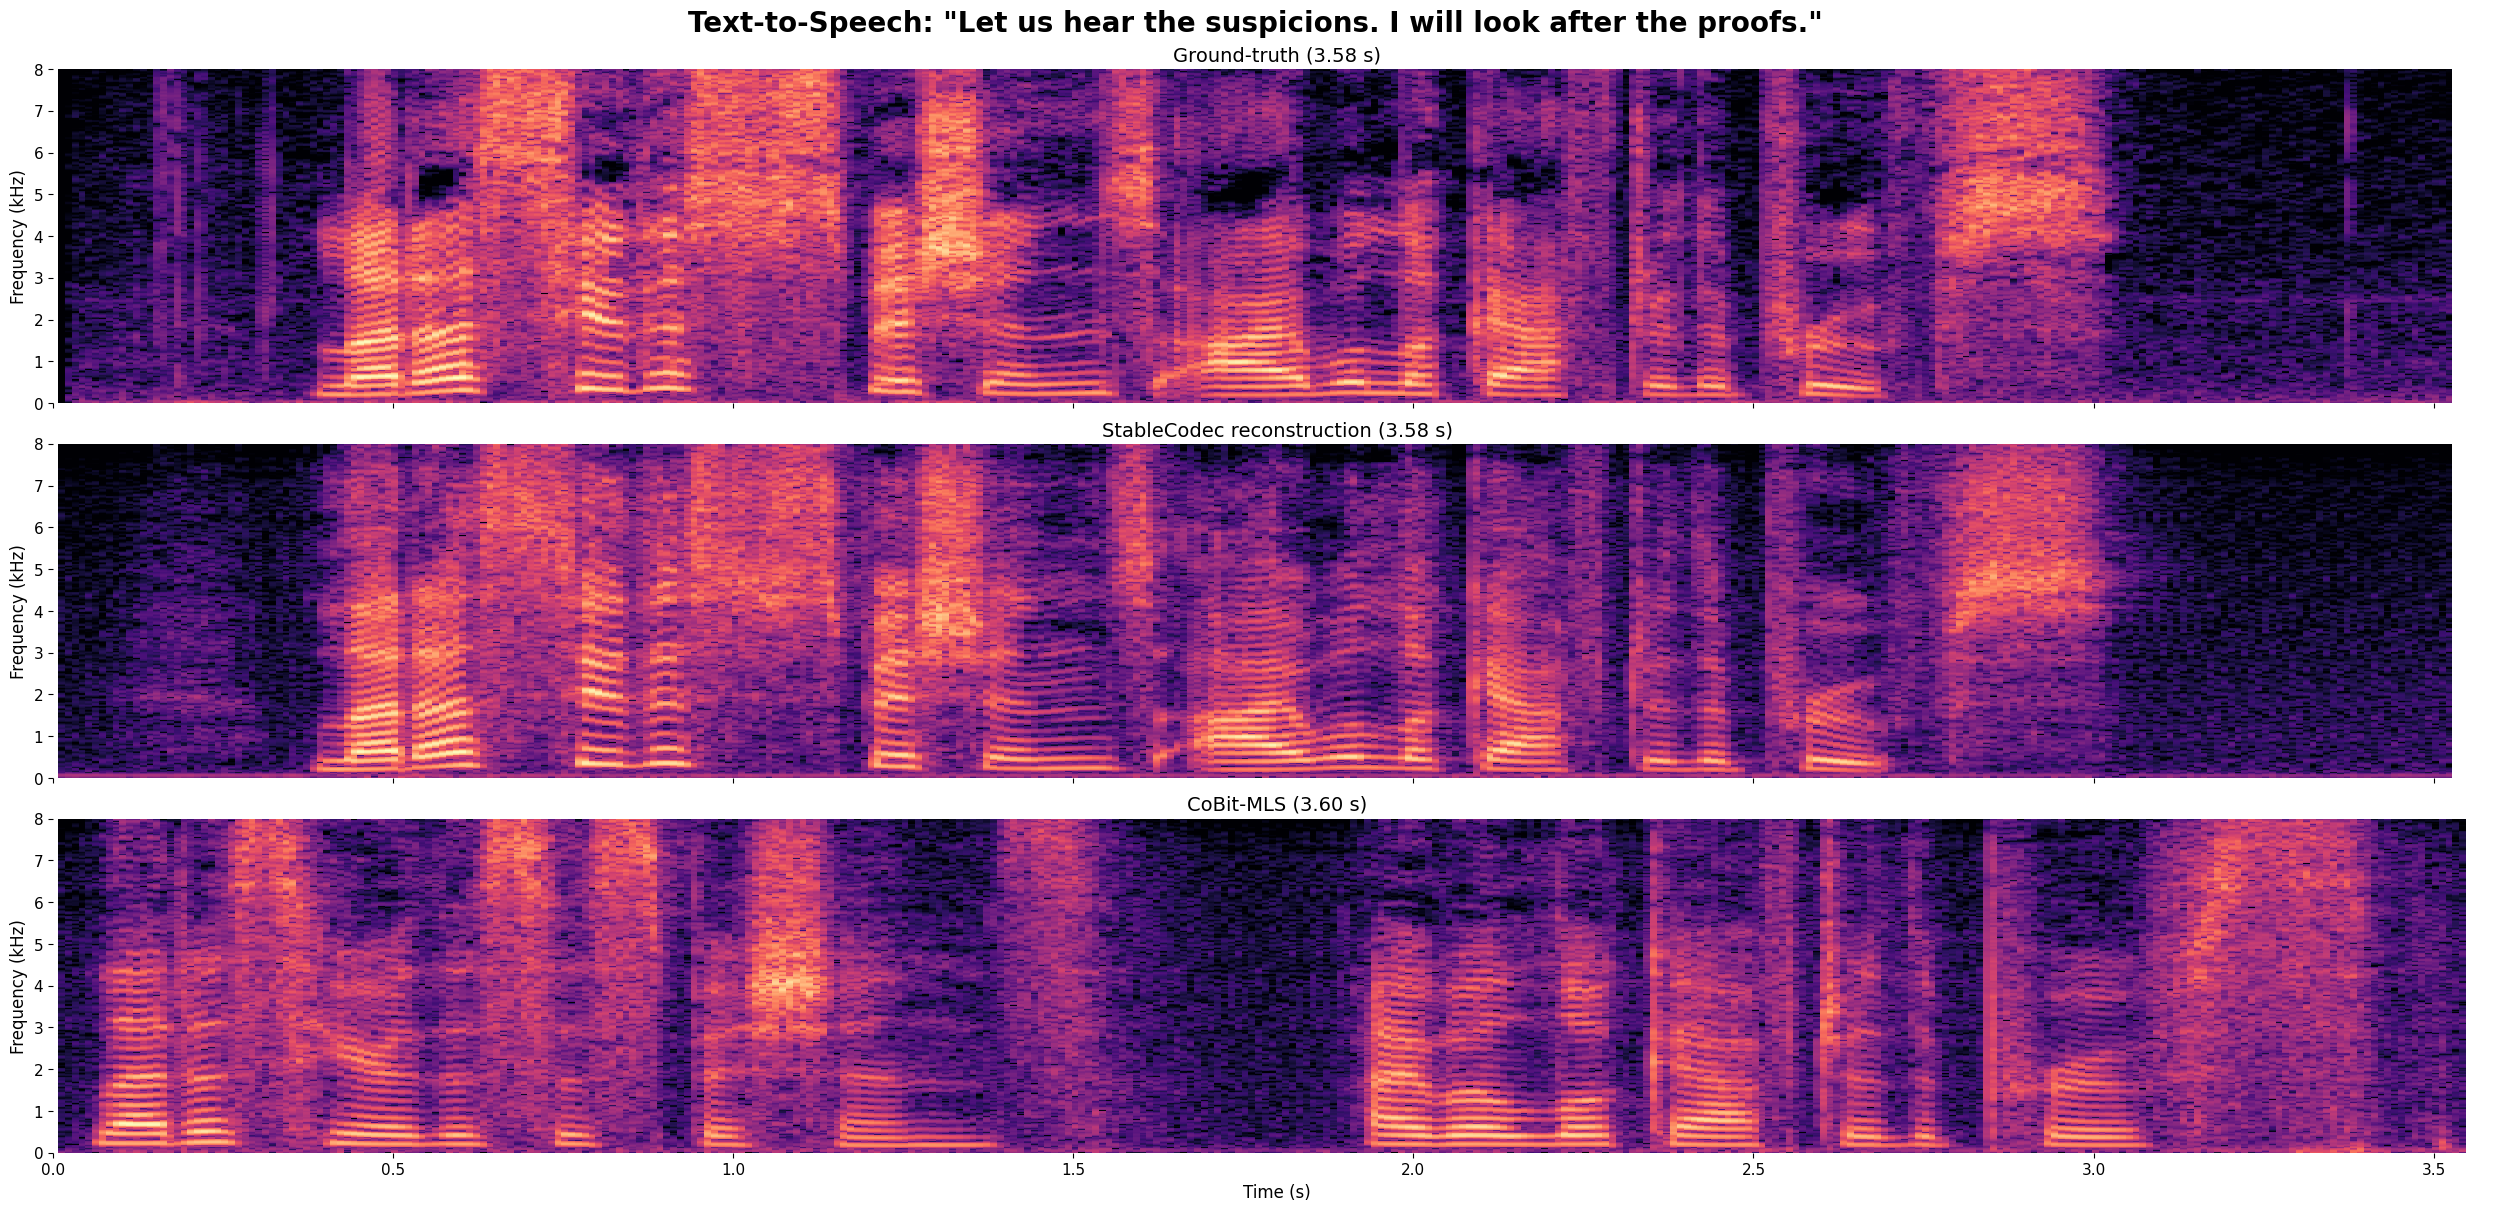
\includegraphics[width=\linewidth]{figures/audio/tts.png}
    \caption{Text-to-speech generation with CoBit-MLS. Given text and speaker tokens (extracted from a held-out example), the model is tasked with generating the speech part of the sequence. The top mel-spectrogram corresponds to the ground truth waveform, the middle one to the StableCodec reconstruction, and the bottom mel-spectrogram to the generated audio by the 633M parameter bitstream diffusion model. The tokenizer introduces visible artifacts, especially at high frequencies. CoBit generation spreads the utterance across a longer time span, without leading and trailing silence, replicating similar frequency patterns. The only exception is the gap between 1.7 and 1.9 seconds, which corresponds to the boundary between sentences.}
    \label{fig:audio:tts-spectrogram}
\end{figure}

\begin{figure} [ht]
    \centering
    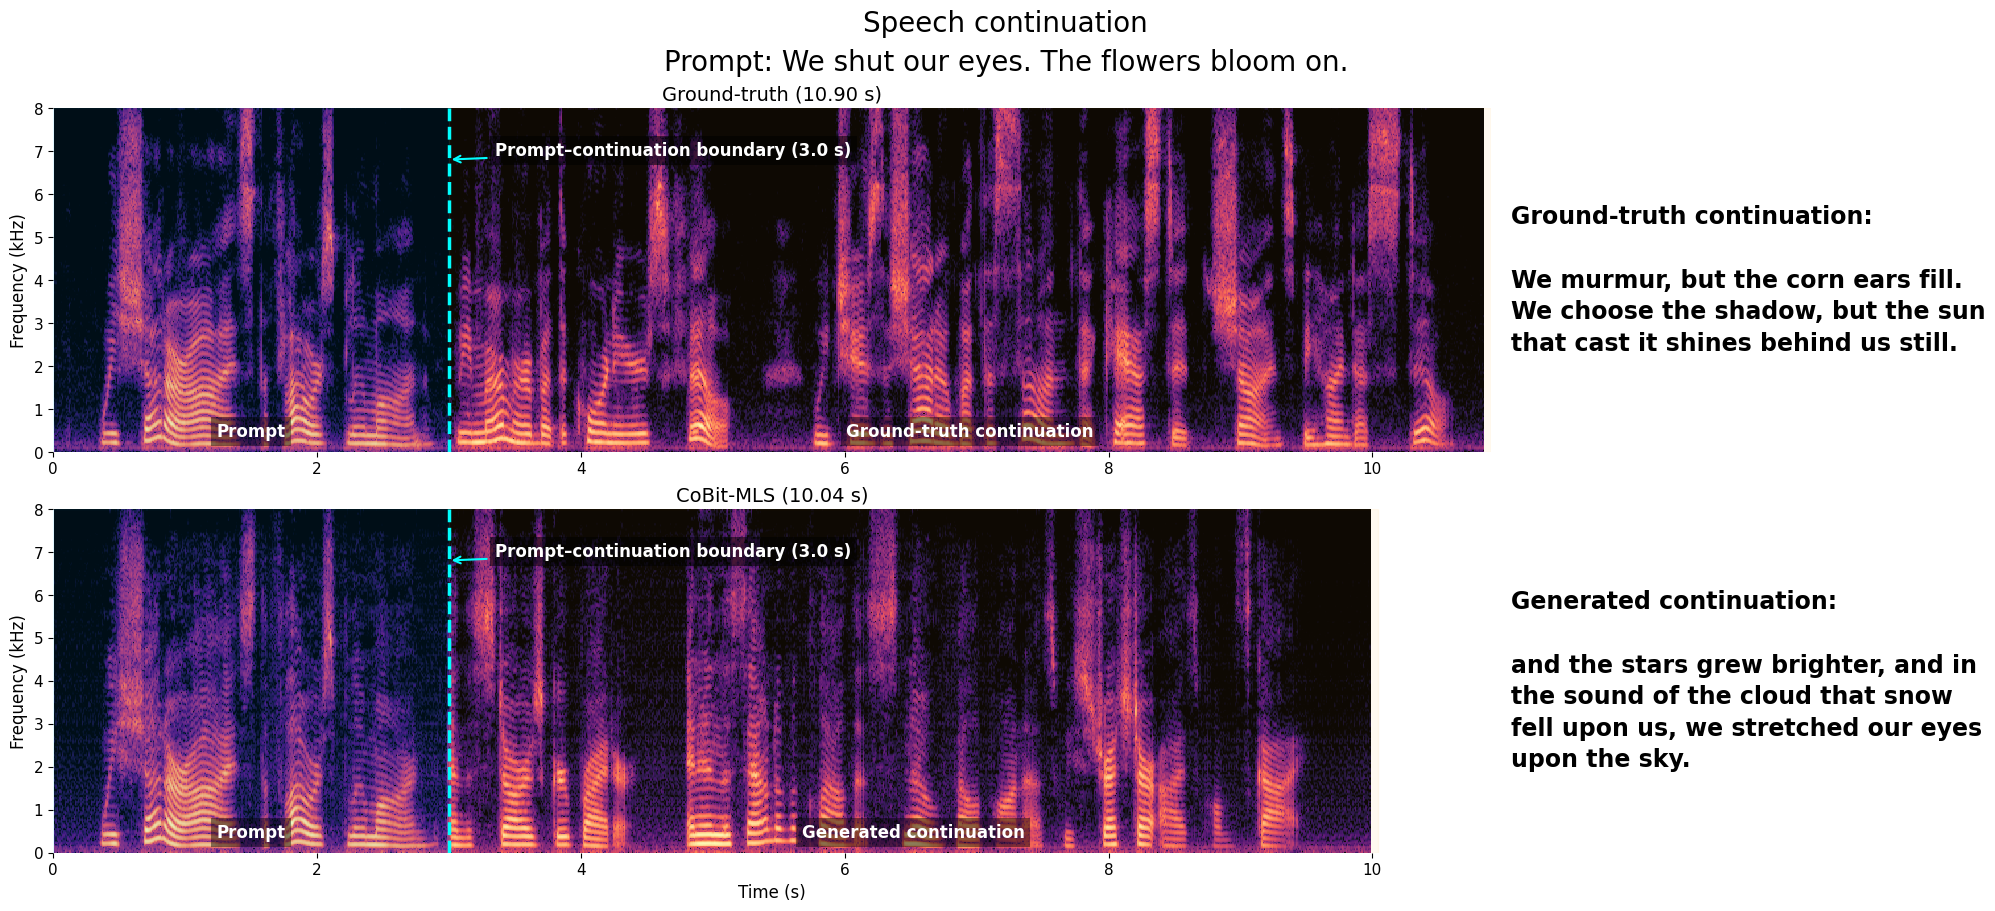
\includegraphics[width=\linewidth]{figures/audio/spectrograms.png}
    \caption{Speech continuation with CoBit-MLS. Given speaker and speech tokens extracted from a 3-second audio prompt, the model is tasked with generating its own continuation. The top mel-spectrogram corresponds to the ground truth continuation, and the bottom mel-spectrogram to the continuation generated by the 633M parameter bitstream diffusion model. The generated spectrogram blends well with the audio prompt, introducing minimal artifacts at the prompt-continuation boundary. Speech continuation is scored not only in terms of acoustic consistency, but also for the semantic relevance and intelligibility of the generated content, shown on the right.}
    \label{fig:audio:continuation-spectrogram}
\end{figure}

\subsection{Sampler Characterisation} \label{app:audio:sampler}

\textbf{Few-step regimes survive only when generating a single modality.} CoBit-MLS step count sweeps for co-generation, cross-modal directions and continuation are reported in Tables \ref{tab:audio:steps:joint}, \ref{tab:audio:steps:cross-modal} and \ref{tab:audio:steps:continuation}, respectively, with fixed stochasticity ($\gamma=0.175$) and guidance (gs=5 for conditional tasks) settings. For text-to-speech, outputs become well-formed from 16 integration steps and approach the model's best performance with 32 steps, particularly on the acoustic elements (UTMOS and SpkSim). Even less compute is required for speech recognition, with strongly sensible transcriptions being produced with as few as 8 steps. Different behavior is observed for joint generation, where all metrics improve near-monotonically with higher NFEs. In few-step regimes, co-generated samples are inaudible; as the step count increases, naturalness improves and the content becomes semantically plausible for both streams, with decreasing perplexity. The same perplexity pattern is observed for speech continuation as well. The model appears to reach an expressiveness optimum at 32 steps, at the expense of semantic degradation. Beyond that point, CoBit continuations already match the tokenizer's speaker similarity ceiling.

\begin{table}[t]
\centering
\small
\setlength{\tabcolsep}{4.5pt}
\begin{tabular}{lrrrrr}
\toprule
\textbf{Steps} & \textbf{WER}$\downarrow$ & \textbf{CER}$\downarrow$ & \textbf{UTMOS}$\uparrow$ & \textbf{GenPPL-Text}$\downarrow$ & \textbf{GenPPL-Speech}$\downarrow$ \\
\midrule
4 & 367 & 250.5 & 1.28 & 20{,}101.9 & 1{,}132.5 \\
8 & 267.8 & 181.4 & 1.31 & 16{,}791.8 & 708.2 \\
16 & 173.4 & 120.5 & 1.51 & 9{,}002.5 & 303.4 \\
24 & 100 & 70.4 & 1.94 & 5{,}377.7 & 440.5 \\
32 & 68 & 47.4 & 2.3 & 3{,}665.2 & 391.4\\
48 & 41.7 & 28.6 & 2.88 & 1{,}857.4 & 359.5\\
64 & 27.8 & 18.5 & 3.12 & 1{,}267 & 313.3 \\
128 & 9.8 & 6.1 & 3.61 & 397.1 & 207.8 \\
256 & 4.8 & 2.6 & 3.75 & 250.4 & 147.2 \\
512 & \textbf{3.8} & \textbf{2.4} & \textbf{3.78} & \textbf{247.2} & \textbf{122.5} \\
\bottomrule
\end{tabular}
\caption{CoBit-MLS joint generation performance at different step counts, computed by generating $1,024$ samples. All rows inject stochasticity at $\gamma=0.175$. Unconditional generation does not use classifier-free guidance, so each integration step corresponds to a single function evaluation.}
\label{tab:audio:steps:joint}
\end{table}

\begin{table}[t]
\centering
\small
\setlength{\tabcolsep}{4.5pt}
\begin{tabular}{lrrrrrr}
\toprule
& \multicolumn{4}{c}{\textbf{Text-to-Speech}} & \multicolumn{2}{c}{\textbf{Speech-to-Text}} \\
\cmidrule(lr){2-5} \cmidrule(lr){6-7}
\textbf{Steps} & \textbf{WER}$\downarrow$ & \textbf{CER}$\downarrow$ & \textbf{UTMOS}$\uparrow$ & \textbf{SpkSim}$\uparrow$ & \makecell{\textbf{WER}$\downarrow$ \\ \textbf{Clean}} & \makecell{\textbf{WER}$\downarrow$ \\ \textbf{Other}} \\
\midrule
4 & 184.2 & 133.3 & 1.51 & 0.05 & 15.4 & 34.9\\
8 & 32 & 21.1 & 3.03 & 0.19 & 9 & 23.9 \\
16 & 6.6 & 4.5 & 3.85 & 0.25 & 8.6 & 23 \\
24 & 6.7 & 4.8 & 3.96 & 0.26 & 8.4 & 22.8 \\
32 & 5.7 & 4 & 3.99 & 0.26 & 8.3 & 22.7 \\
48 & 5.5 & \textbf{3.9} & 4.02 & \textbf{0.27} & 8.3 & 22.9 \\
64 & 6 & 4.1 & \textbf{4.03} & \textbf{0.27} & 8.3 & 22.5 \\
128 & 6.3 & 4.1 & \textbf{4.03} & \textbf{0.27} & \textbf{8.1} & 22.3 \\
256 & \textbf{5.3} & 5.2 & \textbf{4.03} & \textbf{0.27} & 8.2 & 22.4 \\
512 & \textbf{5.3} & 4.1 & 4.01 & 0.26 & 8.2 & \textbf{22.2} \\
\bottomrule
\end{tabular}
\caption{CoBit-MLS cross-modal performance at different step counts, computed by generating $1,024$ samples. All rows inject stochasticity at $\gamma=0.175$. Classifier-free guidance with gs=5 is used throughout the table.}
\label{tab:audio:steps:cross-modal}
\end{table}

\begin{table}[t]
\centering
\small
\setlength{\tabcolsep}{4.5pt}
\begin{tabular}{lrrrrrr}
\toprule
\textbf{Steps} & \textbf{UTMOS}$\uparrow$ & \textbf{FSD-wlm}$\downarrow$ & \textbf{FSD-e2v}$\downarrow$ & \textbf{SpkSim}$\uparrow$ & \textbf{GenPPL-Speech}$\downarrow$ & \textbf{SALMON}$\uparrow$ \\
\midrule
4 & 1.44 & 6{,}001 & 156.2 & 0.05 & 375.1 & 74.58 \\
8 & 1.82 & 3{,}409.6 & 42.1 & 0.14 & 262.6 & 80.08 \\
16 & 3.12 & 2{,}236.3 & 8.9 & 0.3 & 232 & 84.41\\
24 & 3.53 & 2{,}176.6 & 7.1 & 0.33 & 200.9 & 84.41 \\
32 & 3.7 & 2{,}117.6 & \textbf{6.8} & 0.34 & 178.3 & 84.25 \\
48 & 3.83 & 2{,}127.4 & 7.5 & 0.34 & 150.6 & 85.08 \\
64 & 3.88 & 2{,}127.4 & 8.1 & \textbf{0.35} & 130.2 & 84.75 \\
128 & 3.9 & 2{,}108.2 & 9.2 & 0.34 & 111.6 & \textbf{85.58} \\
256 & \textbf{3.91} & \textbf{2{,}108.4} & 10.6 & 0.34 & 94.7 & 84.41 \\
512 & \textbf{3.91} & 2{,}179.3 & 11.8 & 0.34 & \textbf{85.8} & 83.92 \\
\bottomrule
\end{tabular}
\caption{CoBit-MLS speech continuation performance at different step counts, computed by generating $1,024$ samples. All rows inject stochasticity at $\gamma=0.175$. Classifier-free guidance with gs=5 is used throughout the table.}
\label{tab:audio:steps:continuation}
\end{table}

\textbf{Stochasticity is crucial for co-generation.} In Table \ref{tab:audio:deterministic}, we examine the use of a deterministic sampler for CoBit-MLS. For conditional tasks, deterioration compared to a stochastic sampler is minimal, and only apparent in the generative perplexity of speech continuation. In fact, text-to-speech CER, FSD-e2v and SALMON accuracy improve. In joint generation, however, stochasticity is essential: alignment loosens with error rates more than doubling, and the content becomes far less intelligible, especially in the text stream.

\begin{table}[t]
\centering
\small
\setlength{\tabcolsep}{4.5pt}
\resizebox{\linewidth}{!}{%
\begin{tabular}{lrrrrrrr}
\toprule
\textbf{Direction} & \textbf{WER}$\downarrow$ & \textbf{CER}$\downarrow$ & \textbf{UTMOS}$\uparrow$ & \textbf{SpkSim}$\uparrow$ & \textbf{FSD}$\downarrow$ &  \textbf{GenPPL}$\downarrow$ & \textbf{SALMON}$\uparrow$ \\
\midrule
\multicolumn{8}{l}{\emph{Deterministic Sampler}} \\
text $\rightarrow$ speech & 5.9 & 4.1 & 3.97 & 0.26 & --- & --- & --- \\
speech $\rightarrow$ text & 8.6 / 23.4 & 4.7 / 14 & --- & --- & --- & --- & --- \\
speech continuation & --- & --- & 3.85 & 0.33 & 2{,}130.4 / 8.2 & 136.9 & 85.41 \\
joint & 11.3 & 7.3 & 3.54 & --- & --- & 413.9 / 204.2 & --- \\
\midrule
\multicolumn{8}{l}{\emph{Stochastic sampler, $\gamma$=0.175, gs=5}} \\
text $\rightarrow$ speech & 5.3 & 5.2 & 4.03 & 0.27 & --- & --- & --- \\
speech $\rightarrow$ text & 8.2 / 22.4 & 4.3 / 13 & --- & --- & --- & --- & --- \\
speech continuation & --- & --- & 3.91 & 0.34 & 2{,}108.4 / 10.6 & 94.7 & 84.41 \\
joint & 4.8 & 2.6 & 3.75 & --- & --- & 250.4 / 147.2 & --- \\

\bottomrule
\end{tabular}%
}
\caption{CoBit-MLS scores with a deterministic sampler across all four tasks. Integration steps are fixed to 256 and the conditional task use classifier-free guidance with strength 5.}
\label{tab:audio:deterministic}
\end{table}
 
\textbf{FSD deteriorates with guidance.} Tables \ref{tab:audio:guidance:cross-modal} and \ref{tab:audio:guidance:continuation} report guidance sweeps for CoBit-MLS, keeping 256 integration steps and stochasticity $\gamma=0.175$ throughout. While guidance improves modality alignment and generative perplexity, reducing the guidance strength or even shifting to the plain conditional setting improves both FSD metrics, with FSD-e2v surpassing TASLM-Embed for gs=1 and gs=2. Table \ref{tab:audio:guidance:fsd} breaks down FSD calculation. For FSD-wlm, stronger guidance leads to a mean shift; this is natural, as guidance steers generation towards MLS-English, whose pre-processing and frame-level noise may differ substantially from LibriSpeech-PC. For FSD-e2v, only the variance is affected; both datasets consist of reading-style speech and hence contain similar expressiveness.

\begin{table}[t]
\centering
\small
\setlength{\tabcolsep}{4.5pt}
\begin{tabular}{lrrrrrr}
\toprule
& \multicolumn{4}{c}{\textbf{Text-to-Speech}} & \multicolumn{2}{c}{\textbf{Speech-to-Text}} \\
\cmidrule(lr){2-5} \cmidrule(lr){6-7}
\textbf{gs} & \textbf{WER}$\downarrow$ & \textbf{CER}$\downarrow$ & \textbf{UTMOS}$\uparrow$ & \textbf{SpkSim}$\uparrow$ & \makecell{\textbf{WER}$\downarrow$ \\ \textbf{Clean}} & \makecell{\textbf{WER}$\downarrow$ \\ \textbf{Other}} \\
\midrule
1 & 8.6 & 6 & 3.77 & 0.25 & 9.3 & 23.8\\ 
2 & 5.8 & 4.9 & 3.99 & 0.26 & 8.2 & \textbf{22.1} \\
3 & 6.5 & 5.2 & 4.01 & 0.26 & \textbf{8.1} & 22.2 \\
4 & \textbf{5.4} & \textbf{4.5} & \textbf{4.03} & \textbf{0.27} & \textbf{8.1} & 22.2\\
5 & \textbf{5.4} & 5.2 & \textbf{4.03} & \textbf{0.27} & 8.2 & 22.4 \\
\bottomrule
\end{tabular}
\caption{CoBit-MLS cross-modal performance at different guidance scales. All rows use 256 integration steps (256 function evaluations at gs=1; 512 for gs $>$ 1) and stochasticity at $\gamma=0.175$.}
\label{tab:audio:guidance:cross-modal}
\end{table}

\begin{table}[t]
\centering
\small
\setlength{\tabcolsep}{4.5pt}
\begin{tabular}{lrrrrrr}
\toprule
\textbf{gs} & \textbf{UTMOS}$\uparrow$ & \textbf{FSD-wlm}$\downarrow$ & \textbf{FSD-e2v}$\downarrow$ & \textbf{SpkSim}$\uparrow$ & \textbf{GenPPL-Speech}$\downarrow$ & \textbf{SALMON}$\uparrow$ \\
\midrule
1 & 3.88 & \textbf{1{,}953.7} & \textbf{5.1} & 0.33 & 172.1 & 83.41\\
2 & \textbf{3.94} & 2{,}054.1 & 7.8 & 0.34 & 116 & \textbf{85}\\ 
3 & 3.92 & 2{,}073.1 & 9.1 & 0.34 & 116 & \textbf{85} \\
4 & 3.92 & 2{,}140.3 & 10 & 0.34 & 96.1 & 84.83 \\ 
5 & 3.92 & 2{,}108.4 & 10.6 & 0.34 & \textbf{94.7} & 84.41\\
\bottomrule
\end{tabular}
\caption{CoBit-MLS speech continuation performance at different guidance scales. All rows use 256 integration steps (256 function evaluations at gs=1; 512 for gs $>$ 1) and stochasticity at $\gamma=0.175$.}
\label{tab:audio:guidance:continuation}
\end{table}

\begin{table}[t]
\centering
\small
\setlength{\tabcolsep}{4.5pt}
\resizebox{\linewidth}{!}{%
\begin{tabular}{lrrrrrr}
\toprule
& \multicolumn{3}{c}{\textbf{FSD-wlm}} & \multicolumn{3}{c}{\textbf{FSD-e2v}} \\
\cmidrule(lr){2-4} \cmidrule(lr){5-7}
\textbf{gs} & \textbf{Mean Term} & \textbf{Covariance Term} & \textbf{Total} & \textbf{Mean Term} & \textbf{Covariance Term} & \textbf{Total} \\
\midrule
1 & 684.5 & 1{,}269.1 & 1{,}953.7 & 0.19 & 4.86 & 5.05 \\ 
2 & 748.7 & 1{,}305.4 & 2{,}054.1 & 0.3 & 7.51 & 7.81 \\
3 & 756.3 & 1{,}316.8 & 2{,}073.1 & 0.33 & 8.78 & 9.11 \\
4 & 792.7 & 1{,}347.6 & 2{,}140.3 & 0.36 & 9.65 & 10.01 \\
5 & 777.2 & 1{,}331.3 & 2{,}108.5 & 0.37 & 10.24 & 10.61 \\
\midrule
\emph{StableCodec (reconstruction)} & 238.5 & 953.1 & 1{,}119.6 & 0.07 & 1.19 & 1.26 \\
\bottomrule
\end{tabular}%
}
\caption{Breakdown of FSD-wlm and FSD-e2v metrics across the mean term $\|\mu-\mu'\|^2$ and the covariance term $\text{trace}\{\Sigma+\Sigma'-2(\Sigma\Sigma')^\frac{1}{2}\}$ for guidance sweeps. All rows use 256 integration steps (256 function evaluations at gs=1; 512 for gs $>$ 1) and stochasticity at $\gamma=0.175$.}
\label{tab:audio:guidance:fsd}
\end{table}

\subsection{Effect of Model and Corpus Scale} \label{app:audio:scale}

Increasing the model scale and adding MLS-English to the training set improves performance across all tasks and metrics. The only exception is FSD-wlm, where CoBit-LibriTTS benefits from its training set being a subset of the LibriSpeech-PC training partition, and is threrefore more similar to the reference population. MLS-English is much larger (45k hours versus 580), preserves reading-style audio and is part of StableCodec's training corpus as well, reducing the risk of distributional shifts during tokenization. CoBit-MLS is better at aligning text and speech sequences during co-generation, yet CoBit-LibriTTS achieves the best error rates when given the text as input. The performance gap is small for SALMON accuracy, as the smaller model can still capture acoustic properties of the speech prompt. Despite its linguistic fluency and frame-level realism, the main limitation of CoBit-LibriTTS is producing natural-sounding audio, observed across all speech-emitting tasks in terms of UTMOS. In generative perplexity and audio-based metrics for speech continuation, CoBit-LibriTTS even outperforms the 395M parameter Flow-SLM version. For LLM-as-a-Judge, however, CoBit-LibriTTS produces almost exclusively irrelevant continuations.  In SALMON, similar to CoBit-MLS, it scores right between multimodal autoregressive SLMs and speech-only models, except its average accuracy is lower than that of Flow-SLM-S.

\subsection{Speech tokenization and Speaker Features} \label{app:audio:speech-tokenization}

\textbf{StableCodec performance ceiling.} The last rows of Tables \ref{tab:audio:cross-modal}, \ref{tab:audio:continuation} and \ref{tab:audio:salmon} report the evaluation of test set reconstruction with the StableCodec configuration used throughout the text-audio experiments, for all metrics where tokenization determines the best obtainable performance. StableCodec alters the speaker identity and frame-level distribution of the test set substantially, restricting the SpkSim and FSD-wlm scores the model can reach. For speech continuation, CoBit-MLS matches the SpkSim ceiling, while a large portion of its reported FSD-wlm is related to the tokenizer's fidelity. StableCodec's limitated ability to reproduce fine-grained details to the same extent as other tokenizers, such as Mimi, is further observed in the SALMON background-related tasks, where StableCodec reconstruction receives even worse accuracy than all Flow-SLM and Llama-Mimi continuations.

\textbf{Training-inference mismatch.} For all three conditional tasks, BiCodec-global speaker tokens are part of the condition. For ASR, speaker tokens are extracted from the full speech signal, which is always provided as input. Inference-time speaker tokens are extracted from the audio prompt for continuation and from a held-out recording for TTS to rule out information leakage. This is standard practice for zero-shot TTS. During training, however, speaker features from the full ground-truth audio samples are used for all tasks. This forces CoBit to learn a tighter relationship between speaker features and speech tokens, simultaneously accounting for the variability in BiCodec-global, which does not guarantee that all recordings of the same speaker produce identical outputs. A training-inference mismatch is therefore introduced to facilitate unified training. Table \ref{tab:audio:spksim} documents the change in performance if the same type of ground-truth speaker tokens are used during inference (note that this is conducted solely to quantify the effect of ground-truth speaker tokens; it includes information leakage and cannot be considered a valid evaluation for CoBit). Speaker similarity increases from 0.27 to 0.32, still well below GPA-v1.5. The held-out samples themselves are much more similar to the ground truth test examples, with SpkSim well beyond StableCodec's ceiling.

\begin{table}[t]
\centering
\small
\setlength{\tabcolsep}{4.5pt}
\begin{tabular}{lrrrr}
\toprule
 & \textbf{WER}$\downarrow$ & \textbf{CER}$\downarrow$ & \textbf{UTMOS}$\uparrow$ & \textbf{SpkSim}$\uparrow$ \\
\midrule
\multicolumn{5}{l}{\emph{CoBit-MLS, Steps=512, $\gamma=0.27$, gs=5}} \\
held-out features & 5.3 & 4.1 & 4 & 0.27 \\
ground-truth features & 5.2 & 3.6 & 4.03 & 0.32 \\
\midrule
\emph{Held-out vs. ground truth samples} & --- & --- & --- & 0.65 \\
\bottomrule
\end{tabular}
\caption{Effect of speaker tokens on text-to-speech performance. Both CoBit-MLS rows are obtained from text-to-speech generation.}
\label{tab:audio:spksim}
\end{table}

\textbf{Co-generation: Speaker Realization.} During joint generation, CoBit samples speaker tokens, yet it does not use them for waveform decoding. To measure how speaker conditioning is realized to audio, we compare the sampled speaker tokens to the ones BiCodec-global extracts from the decoded waveform for CoBit-MLS; results are shown in Table \ref{tab:audio:realized-conditioning}. Sampled and realized token sequences agree on 7.62\% of the total tokens, which corresponds to 2-3 tokens per example. Since BiCodec-global is FSQ-based, disagreement in a single latent dimension produces an entirely different token, and thus the token agreement rate is highly sensitive to StableCodec artifacts, that, as already discussed for SpkSim, are recognizable for ECAPA-TDNN, which BiCodec-global is also based on. For this reason, we also examine the relationship between latent BiCodec-global representations that correspond to the FSQ codes, in terms of RMSE and cosine similarity (because FSQ bounds each latent dimension, RMSE can be normalized with respect to the highest attainable value). Sampled and realized continuous latents are closely aligned, showing that CoBit-MLS learns to realize its speaker conditioning, despite not reproducing exact BiCodec-global sequences. The top left panel of Figure \ref{fig:audio:speaker} also verifies that this behavior is observed for the majority of the samples and is not driven by outliers.  

\begin{table}[t]
\centering
\small
\setlength{\tabcolsep}{4.5pt}
\begin{tabular}{lrrrr}
\toprule
& \textbf{Token Agreement(\%)} & \textbf{Position RMSE(\%)} & \textbf{Sequence RMSE(\%)} & \textbf{Cosine Similarity}\\
\midrule
Paired & 7.62 & 5.08 & 5.69 & 0.785 \\
Shuffled & 0.26 ($\pm$0.03) & 10.58 ($\pm$0.03) & 10.99 ($\pm$0.03) & 0.222 ($\pm$0.005) \\
\bottomrule
\end{tabular}
\caption{Speaker conditioning realization for CoBit-MLS co-generation. Comparisons are drawn between BiCodec-global representations CoBit-MLS samples directly (speaker positions in its generated sequence) and BiCodec-global representations extracted from the waveforms CoBit-MLS generates. RMSE and cosine similarity metrics are computed on BiCodec-global's latent space by transforming each FSQ code into its underlying latent vector. The first row computes paired sample correspondence (generated and realized representations for the same sequence); the second row gives a shuffled baseline for shuffled examples, averaged over 100 draws. Cosine similarity is averaged across 32 sequence positions and 1024 samples.}
\label{tab:audio:realized-conditioning}
\end{table}

\textbf{Co-generation: speaker diversity.} For co-generation, we are also interested in whether CoBit can actually learn to draw random voices, instead of repeating a small set of identities. To test this, we calculate the similarity among generated populations under an external speaker verification system that is unrelated to ECAPA-TDNN and BiCodec, namely CAM++ \citep{audio:campp}. We compare CoBit-LibriTTS and CoBit-MLS with the cascaded joint generation pipeline (Appendix \ref{app:audio:baselines}), which learns to autoregressively sample speaker tokens using the same training set and representation as CoBit-MLS and realizes speaker conditioning via the BiCodec decoder. Results are reported in Table \ref{tab:audio:diversity} and the distributions of within-distribution pairwise cosine similarity are visualized in the bottom panel of Figure \ref{fig:audio:speaker}. CoBit-MLS generates as diverse speakers as the baseline on average, with significant overlap in their similarity distributions; CoBit-LibriTTS, having been trained on a much narrower speaker collection, is heavily limited in the range of voices it can reproduce.

\begin{table}[t]
\centering
\footnotesize
\setlength{\tabcolsep}{4pt}
\begin{tabular}{lrrr}
\toprule
& \multicolumn{2}{c}{\textbf{BiCodec-global}} & \textbf{CAM++} \\
\cmidrule(lr){2-3} \cmidrule(lr){4-4}
\textbf{Model} & \textbf{Entropy(bits)} & \textbf{Cosine Similarity (sampled)} & \textbf{Cosine Similarity (realized)} \\
\midrule
\multicolumn{4}{l}{\emph{CoBit (ours; from scratch, no pretrained components)}} \\
CoBit-LibriTTS & --- & --- & 0.439 \\ 8.64 & 0.27 & 0.295 \\
CoBit-MLS & 8.64 & 0.27 & 0.295 \\
\midrule
\multicolumn{4}{l}{\emph{Autoregressive System (SmolLM+Speaker $\rightarrow$ SparkTTS)}} \\
Cascade & --- & --- & 0.29 \\
\midrule
\multicolumn{4}{l}{\emph{LibriTTS+MLS-English}} \\
Matched Population & 8.75 ($\pm$0.01) & 0.3 ($\pm$0.002) & --- \\
Full & 9.97 & --- & ---\\
\bottomrule
\end{tabular}
\caption{Co-generation speaker diversity, measured in terms of speaker-token entropy and cosine similarity of the sampled BiCodec-global latents and the extracted CAM++ embeddings. Matched population statistics for the training set are computed using 100 random draws.}
\label{tab:audio:diversity}
\end{table}

\begin{figure}[ht]
    \centering
    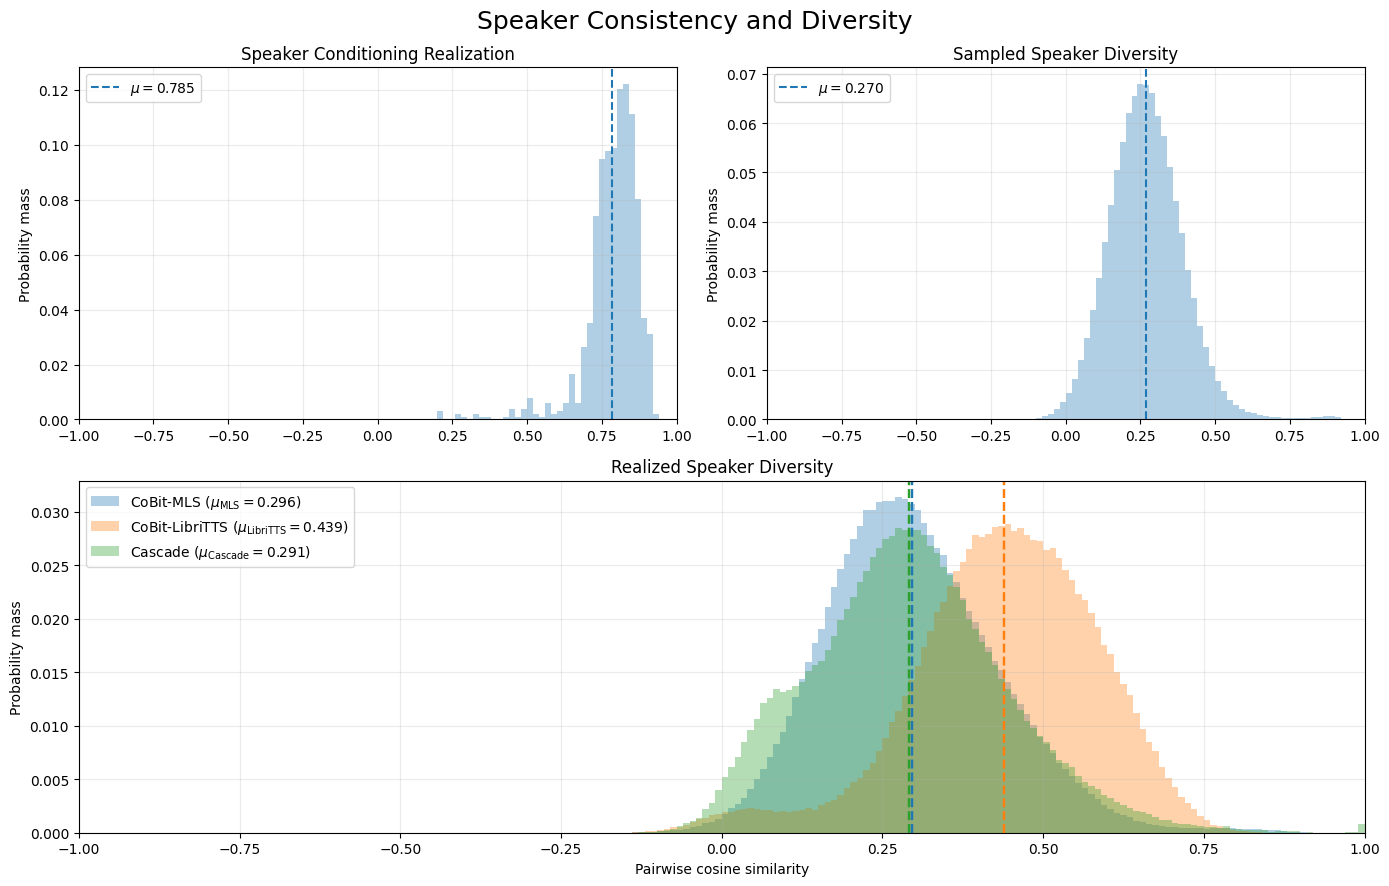
\includegraphics[width=\linewidth]{figures/audio/speaker.png}
    \caption{Speaker consistency and diversity distribution for co-generation, in terms of latent space cosine similarity. Top left: Per-sample embedding similarity between BiCodec-global FSQ components sampled by CoBit-MLS (Steps=512, $\gamma=0.175$) during co-generation and BiCodec-global FSQ components extracted from the generated waveforms (decoded StableCodec tokens). Top right: Embedding similarity of BiCodec-global FSQ components across the 1{,}024 BiCodec-global sequences sampled by CoBit-MLS. Both plots are averaged over sequence positions. Bottom: realized speaker diversity among the generated populations of CoBit-MLS, CoBit-LibriTTS (Steps=256, $\gamma=0.175$) and the SmolLM-Speaker-SparkTTS autoregressive cascade (Appendix \ref{app:audio:baselines}), measured in terms of embeddings from the speaker verification CAM++ checkpoint.}
    \label{fig:audio:speaker}
\end{figure}

\textbf{Text-to-speech: speaker realization.} We also evaluate the model's ability to realize different voices in text-to-speech transfer, by generating audio for the same 10 text prompts with all 39 speakers of LibriSpeech-PC test-clean. Figure \ref{fig:audio:tts-vc} shows how SpkSim and UTMOS scores are distributed across the different speakers. For some speakers, the BiCodec-global representation translates better than others, with speaker similarities ranging from 0.1 to 0.8; UTMOS values are 

\subsection{Speech Recognition Error Breakdown} \label{app:audio:asr}

Speech-to-text is the task where cold initialization is the most apparent, as it contradicts the design of ASR-specific systems, which typically recognize speech at character, token, or phoneme level, and then employ a text language model to decode the output into well-structured sentences. For SLMs, the textually pretrained transformer trunk implicitly plays a similar role, leading to more coherent transcriptions, as previously demonstrated by \cite{audio:voxtlm}. Figure \ref{fig:audio:asr} separates CoBit-MLS speech-to-text errors into substitutions, insertions and deletions. The vast majority of word-level errors are substitutions: the model very rarely hallucinates additional words or skips existing ones; it just lacks the language modeling capacity to leverage character- and word-level context to achieve more accurate recognition.

\begin{figure}[ht]
    \centering
    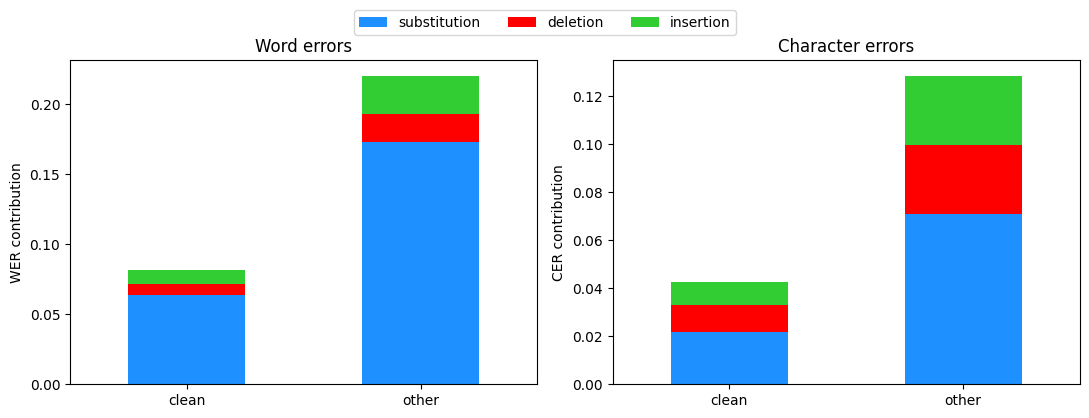
\includegraphics[width=\linewidth]{figures/audio/asr_breakdown.png}
    \caption{Breakdown of speech-to-text WER and CER for CoBit-MLS, using the selected setting in Table \ref{tab:audio:operating-points}.}
    \label{fig:audio:asr}
\end{figure}

\subsection{LLM-as-a-Judge Score Distributions} \label{app:audio:llm}

Per-model distributions of LLM-as-a-Judge scores are shown in Figure \ref{fig:audio:llm-judge}. CoBit-MLS produces relevant continuations 39\% of the time, yet even then relevance to the prompt's theme is only marginal. CoBit-LibriTTS produces almost exclusively irrelevant continuations. Nonetheless, both models score on average higher than Flow-SLM-S, which receives the worst score of any studied SLM. CoBit is trained from scratch and only sees storybook passages, whose content is very difficult to generalize, even to other stories. Text pretraining effectively exposes SLMs to much richer semantics, as text-only corpora are typically more diverse. Even warm initialization, however, appears to be insufficient for semantic extrapolation; thematically accurate speech is only achieved by TASLM-Embed, which uses text-aligned speech representations that close the semantic gap between text and speech modeling.

\begin{figure}[ht]
    \centering
    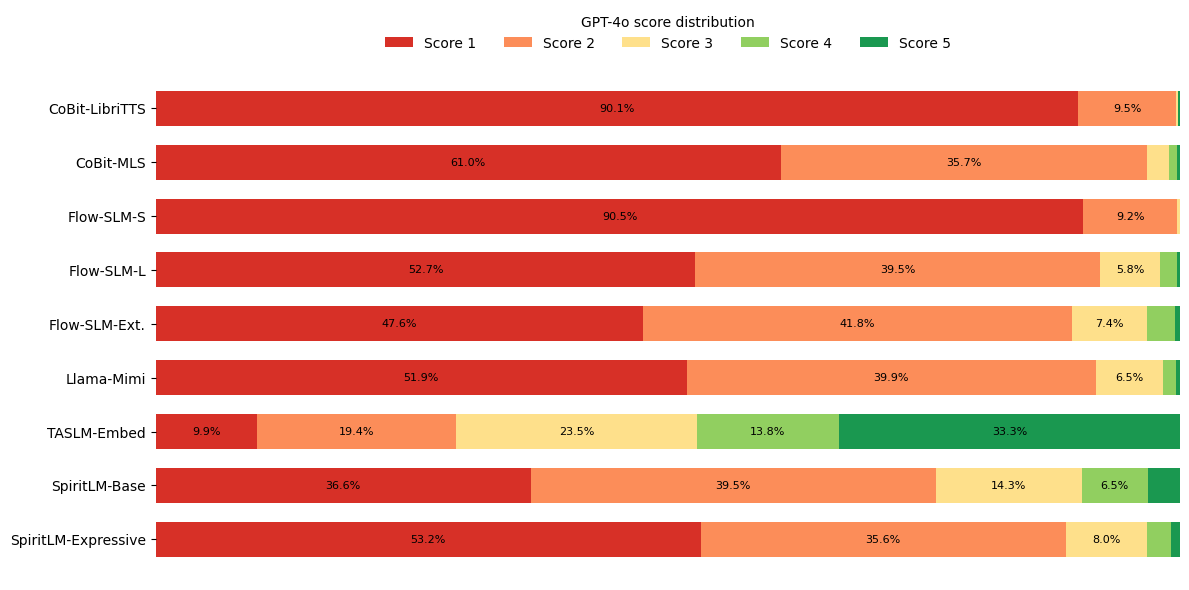
\includegraphics[width=\linewidth]{figures/audio/llm-judge-distribution.png}
    \caption{LLM-as-a-Judge score distribution for CoBit and autoregressive SLMs. CoBit-LibriTTS almost always receives the lowest possible score. A large portion of CoBit-MLS samples perform moderately better, but neither of the model can consistently achieve scores of 3 or higher.}
    \label{fig:audio:llm-judge}
\end{figure}


\subsection{Baseline Systems} \label{app:audio:baselines}

The SLM baselines considered in this work are autoregressive; diffusion models in speech generation are mostly limited to TTS systems or ASR-TTS hybrids. 

\textbf{Multimodal SLMs and Hybrids.} The most comparable text-audio baselines for CoBit are models that learn to generate both text and speech. TASLM \citep{audio:taste} generates the two modalities jointly, leveraging continuous text-aligned speech representations from the TASTE encoder and implementing separate prediction heads. The semantic equivalence of text units and speech embeddings bridges the gap between audio and text generation, producing linguistically fluent and conceptually consistent audio. Other approaches focus on systems that can be extended to cross-modal tasks. SpiritLM \citep{audio:spirit-lm} is trained on interleaved text-audio sequences, and has an expressive variant with additional control over pitch and style. SpiritLM models can perform TTS and ASR via task-specific fine-tuning and few-shot prompting. Moshi \citep{audio:moshi} is a spoken dialogue system that produces text alongside speech as an inner monologue that steers generation towards intelligible sentences. Its cross-modal capabilities arise from a time delay on the generated stream and inference-time teacher-forcing on the conditioning stream. GPA \citep{audio:gpa} is a multi-task autoregressive hybrid that treats TTS and ASR as conditional language modelling problems. It is the closest method to CoBit in terms of scale, multi-task joint training and initialization from scratch, but it is limited to cross-conditional tasks and cannot perform speech language modelling. However, all of these models require task-specific design and modifications for TTS and ASR, in contrast to CoBit.

\textbf{Speech-only SLMs.} In the context of speech generation, additional comparisons can be drawn to textless SLMs, which mainly rely on the powerful Mimi tokenizer to balance semantic information with fine-grained acoustic detail. Llama-Mimi \citep{audio:llama-mimi} autoregressively predicts each Mimi layer, leveraging RVQ's conditional nature: the generation of each code is conditioned on both the previous tokens and the earlier codebooks of the same token. Flow-SLM \citep{audio:flow-slm} exploits Mimi's semantic-acoustic combination for cascaded prediction, breaking the strictly autoregressive paradigm: a causal transformer predicts the semantically distilled first RVQ layer; then, unquantized Mimi embeddings are inferred with flow matching, conditional on look-ahead semantic tokens.

\textbf{Cascaded Co-generation.} None of the multimodal systems are evaluated on unconditional co-generation. TASLM-Embed and Moshi are the only baselines that are, in theory, capable of true parallel generation, but they are not trained for such a task. Matching the autoregressive nature of all other baselines, we instead compare CoBit to a cascaded pipeline: text is generated unconditionally with a text LM and speaker identity is sampled from a small transformer; a TTS system then uses the text and speaker features to synthesize the speech sequence. This cascade system effectively targets the same distribution as CoBit for joint generation, factorized as $p(\text{text, speaker, speech}) = p(\text{text})p(\text{speaker})p(\text{speech}|\text{text, speaker})$. To match the $630$M parameter scale of CoBit, SmolLM2-135M \citep{audio:smollm} is used for text generation and Spark-TTS \citep{audio:spark-tts} is used for speech synthesis. Speaker features are sampled by a transformer with 1M parameters in the form of BiCodec-global tokens and passed to the Spark-TTS decoder. We train the speaker transformer on LibriTTS and MLS-English. All three components of the cascade are autoregressive. A known drawback is that unconditional generation with a generic text LM can lead to web or code artifacts that cannot be synthesized naturally as speech, causing very high GenPPL-Speech, as observed in Table \ref{tab:audio:joint}.

\subsection{Measurement Comparability} \label{app:audio:comparability}

For speech continuation and co-generation, we evaluate all baselines under the same protocol as CoBit using publicly available checkpoints. For cross-modal transfer, we only evaluate GPA-v1.5. While public SpiritLM and Moshi models do exist, their TTS and ASR performance relies on task-specific fine-tuning and engineering modifications (\ref{app:audio:baselines}) that cannot be reproduced exactly from public checkpoints; we therefore report results from their respective papers. All generation-based SALMON scores are taken directly from \cite{audio:gen-salmon}. However, the exact protocol documented in the original work is replicated, using the same checkpoints for the judge models.
 
\section{Protein sequence and structure experiments}
\label{app:protein}
\subsection{Training, representation and evaluation protocol}
\label{app:protein:protocol}


\subsection{Metrics}
\label{app:protein:metrics}


\subsection{Metrics}
\label{app:protein:pareto}

\subsection{Comparison}
\label{app:protein:comparison}


\end{document}
